\documentclass [10pt,letterpaper]{report}
%\documentclass[10pt,letterpaper]{article}
%\documentclass[10pt,letterpaper,twocolumn]{article}
%
%\documentclass[10pt,letterpaper,twocolumn]{report}
%\documentclass[10pt,letterpaper]{report}
%
%\usepackage[greek,english]{babel}
\usepackage[greek,english]{babel}
\usepackage[T1]{fontenc}
\usepackage{graphicx}
\usepackage{color}
\usepackage{wrapfig}


\textheight     =  8.4in
\textwidth      =  6.8in
%\parindent      =  0.0cm

\topmargin      =  -0.2in
\oddsidemargin  =  -0.2in
\evensidemargin =  -0.2in
%\hoffset        =  0.0cm
%\voffset        =  0.0cm

\newcommand{\nuSolve}{\greektext n\latintext Solve}
\newcommand{\thisVersion}{0.8.2}

\graphicspath{{graphics/}}

\begin{document}

\title{\nuSolve{}-\thisVersion{}: User Guide}

\author{
Sergei Bolotin,
Karen Baver,
John Gipson,
David Gordon,
Daniel MacMillan
}

\date{\today}


\maketitle

\tableofcontents


\def\leftSp      {48mm}
\def\riteSp     {113mm}


\chapter{Introduction}
\label{intro}




%%%%%%%%%%%%%%%%%%%%%%%%%%%%%%%%%%%%%%%%%%%%%%%%%%%%%%%%%%%%%%%%%%%%%%%%%%%%
%%
%%
%%
%%%%%%%%%%%%%%%%%%%%%%%%%%%%%%%%%%%%%%%%%%%%%%%%%%%%%%%%%%%%%%%%%%%%%%%%%%%%
\section{VLBI data analysis software}

This document describes how to use the geodetic VLBI software \nuSolve{}.
If a term <<geodetic VLBI>> is unfamiliar to you, you probably confused
\nuSolve{} with some other software. It is designed for processing of a
single geodetic VLBI session.

\nuSolve{} is a replacement of the interactive mode of SOLVE. In this
case it works in cooperation the with CALC/SOLVE system. It can also
work in standalone mode, in which case it is independent of CALC/SOLVE,
and CALC/SOLVE do not need to be installed on your computer. The
standalone mode could be useful for VLBI data analysis centers that use
their own software and want to generate their own version 4 database.

This is an initial version of the user guide, so many things are not
covered and we assume that a user is familiar with CALC/SOLVE. Later,
we will extend its content. Additional information on \nuSolve{} can be
found in \cite{Bolotin2010}, \cite{Bolotin2011} and \cite{Bolotin2012}.

The guide covers {\thisVersion{}} version of the software. In the older
versions, perhaps, not fully implemented all features described here.
On the other hand, if you use newer version of \nuSolve{} it is worth
to find an updated version of the guide too (if it exists).

As it was stated above, \nuSolve{} is designed to process a single
session of VLBI observations. The main purpose of the software is to
prepare a newly available VLBI session for further analysis. In general,
this preliminary analysis needs to be done only once for a particular
session.





%%%%%%%%%%%%%%%%%%%%%%%%%%%%%%%%%%%%%%%%%%%%%%%%%%%%%%%%%%%%%%%%%%%%%%%%%%%%
%%
%%
%%
%%%%%%%%%%%%%%%%%%%%%%%%%%%%%%%%%%%%%%%%%%%%%%%%%%%%%%%%%%%%%%%%%%%%%%%%%%%%
\section{Requirements}
\label{intro_reqs}

\subsection{Hardware requirements}
There is no special requirements to the hardware. Though, a good monitor
with decent resolution will be helpful, \nuSolve{} uses GUI to display
and let a user to edit VLBI observations.


\subsection{Software requirements}
The software was developed using GNU/Linux operating system, however it
does not use any Linux-specific functions, so it should be easily
adjusted to work with other POSIX compatible operating systems.

Speaking about Linux, we would suggest to use modern distribution (and
make updates on a regular basis), but \nuSolve{} can be compiled and run
on an ancient systems too.

The software uses several external packages: Qt, netCDF and, optionally,
HOPS and libCalc.

The library Qt provides graphical user interface and basic tools.
Modern Linux distributions provide Qt, a user have to add development
files (C++ header files, utilities, etc.) from the corresponding
packages. Consult your system administrator for details. Currently,
the version 5 of Qt library, Qt5, is necessary to compile and link
the software. The previous version of Qt, Qt4, was used in earlier
versions of \nuSolve{} distributions but is not supported any more.

Since most of modern distribution ship Qt5 as a default library,
no additional keys are required to use the library with \nuSolve{}.

The netCDF package provides access
to files in netCDF format. This representation of data was chosen to store
data in vgosDb format. The netCDF library also is available with modern
Linux distributions. As an alternative, a user can install it from the
sources available at
\begin{center}
ftp://ftp.unidata.ucar.edu/pub/netcdf/
\end{center}
\noindent
Neither \nuSolve{} nor CALC/SOLVE use features that appeared in version 4
or higher of the netCDF library.

The software Haystack Observatory Postprocessing System (HOPS) is required
for vgosDbMake utility. You can skip it if you do not want to compile this
utility. The distribution package of HOPS is at
\begin{center}
ftp://gemini.haystack.mit.edu/pub/hops/
\end{center}
\noindent
The software is distributed in sources. Version 3.12 or higher of HOPS
distribution should be used.

A librarized version of CALC, libCalc, is necessary to compile vgosDbCalc.
Previously, libCalc was a part of nuSolve distribution. With the version
0.8.0 of the distribution it was decoupled from nusolve package.
The library is available at
\begin{center}
{\tt
https://sourceforge.net/projects/libcalc/
}
\end{center}



%%%%%%%%%%%%%%%%%%%%%%%%%%%%%%%%%%%%%%%%%%%%%%%%%%%%%%%%%%%%%%%%%%%%%%%%%%%%
%%
%%
%%
%%%%%%%%%%%%%%%%%%%%%%%%%%%%%%%%%%%%%%%%%%%%%%%%%%%%%%%%%%%%%%%%%%%%%%%%%%%%
\section{Changes from previous versions}
\label{intro_changes}

This section was added in 0.5.0 version of the distribution (version 0.5.0
of the \nuSolve{} user guide). It covers changes in the software and the user
guide.


\subsection{Changes in version 0.8.3}

This is mostly a bug fixing release. The calculations of ionosphere effective
frequencies and corrections were modified to use channel bandwidth in a proper
way. The applied sigmas of delays now evaluated according to Joh's memo 
(see docs/Ionosphere.pdf of the distribution).

Output of data in ANTCAL format now in version 2 of the format (see
docs/antcal\_specs-v2.txt). Many small bugs were fixed.


\subsection{Changes in version 0.8.2}

The sections {\emph{\ref{section-software-prefs} The software preferences}
and {\emph{\ref{sect-session-editor} Session Editor} were updated to reflect
the latest changes in software configuration and session editor.

A user can specify extensions for master file names and order to search, subsection
\emph{\ref{prefs-general} Specifying directories, external files}
was updated to reflect the changes.

% version to read:
If a user has provided session name to read, nuSolve can filter out wrapper files
that were produced by other analysis centers even if the wrapper files have higher
version number, see subsection
\emph{\ref{prefs-options} Software options}
for the details.

% cable cal origin and types:
Cable calibration corrections origin is added to the list of stations, a user
can cahnge the origin of cable calibraiton corrections (if data are available), see
subsection
\ref{subsect-sessedit-stations-list} Tab <<Stations (List)>>}.



\subsection{Changes in version 0.8.1}
A couple of bugs in the software were fixed, there are no visble changes to
the User Guide.


\subsection{Changes in version 0.8.0}
Due to forthcoming licensing requirements the sources of CALC and nuSolve are
decoupled. To compile vgosDbCalc a user have to install libCalc first. The sources
of vgosDbCalc now does not contain CALC codes. In the case if libCalc is missing,
the utility will not be configured and compiled.
Chapter \emph{\ref{chapter-installation} Installation} was modified to reflect this
change.

All external source codes (about a dozen of functions, external and derived
from SOLVE sources) were replaced with the the independent source code.

Starting with this version, nuSolve supports version 2 of masterfile format and
new database naming convention.


\subsection{Changes in version 0.7.6}
The release contains few bugfixes: update of {\it configure} script and sources
to work with GCC 12.1 (thanks to Leonid Petrov); proper designation of CDMS cable
calibration type when the data were extracted from FS log files (thanks to Arthur
Niell); changing of a name of vgosDb variable that accumulates cable calibration
of different types (thanks to Haystack VLBI group).

\subsection{Changes in version 0.7.5}
This version introduces multi-thread matrix triangulation. For multi-core CPU such
parallel computations will decrease time of processing a session. See Chapter
\emph{\ref{chapter-invokation} Invoking \nuSolve{}} for the details.

GUI is added to plot all available cable calibration corrections. Also, a user
can control what type of the correction should be used in a solution. It can be
set up for a whole session or on a per station basis. The subsection
\emph{\ref{subsubsect-sessedit-station-attr-editor} Station Attributes Editor}
discusses how the type of cable calibration corrections can be changed using GUI
mode of the software. The script mode support of this feature is covered in
subsections \emph{\ref{section-scripting-config} Solution configuration in scripts}
and
subsections \emph{\ref{section-scripting-session-station} The object <<Station>>}.

A station attribute "bad meteo parameters" is added. If it is set, then a "standard"
values of temperature, pressure, and relative humidity are using in a solution.
This option is discussed in subsection
\emph{\ref{subsect-sessedit-stations-list} Tab <<Stations (List)>>} for GUI mode
and in subsections
\emph{\ref{section-scripting-session-station} The object <<Station>>} for script mode.


Sources of the plotter subsystem has been modified so the software can be
compiled with Qt5 version 5.12 or older.

The spoolfile file output was updated: a name of reported database now does
not depend on a primary band (will work for databases with names like 22MAY16MH).



\subsection{Changes in version 0.7.4}

Various bugs have been fixed.

The command line arguments parser has switched to ARGP from GNU C Library.

The plotting subsystem now can save plots in raster formats (JPG, PNG, PPM).
The subsection
\emph{\ref{prefs-general} Specifying directories, external files},
\emph{\ref{prefs-options} Software options},
\emph{\ref{prefs-uids} User's identities} and 
\emph{\ref{prefs-options-logger} Configuration of logging subsystem}
were refreshed.

For testing purposes the following options were added. The fly-by mapping
function can be calculated as MTT or NMF mapping function. The software can
read external EOP files (implemented formats: USNO and IERS EOP). For details
see \emph{\ref{sect-config-models} Applying different models and using external
a priori information}.

The Chapter
\emph{\ref{chapter-scripting} Scripting support}
was updated to refresh changes in the script mode.


\subsection{Changes in version 0.7.3}
The configure script has been reworked. A mandatory option {\tt -{}-with-calc-datadir=}
is added, see details in Chapter \emph{\ref{chapter-installation} Installation}.

The script that converts vgosDb to and from vgosDa format, vgosDxConvertor, has
been reworked, Section
\emph{\ref{section-using-script-converts} Converting data format of a VLBI session}
was refreshed.

\subsection{Changes in version 0.7.2}

A new utility, log2ant, is added to the distribution. It extracts various sensors
readings from a station log file and stores them in ANTCAL format. See log2ant User
Guide for details.

The utility vgosDbProcLogs extracts and stores in vgosDb format tsys data (if
available).

The software now requires Qt5, the realization of regular expressions in Qt4 is too slow.

An option to generate a list of commands to refringe selected by a user observations is
implemented. It should be useful to deal with subambiguities.

The General Configure Editor was modified to allow a user to control using of observations
with fourfit error codes <<G>> and <<H>>.

In Preferences, Logger Options, an option to print full date in the log output is added.


\subsection{Changes in version 0.7.1}

The distribution has switched to Qt5 as a default version of Qt library. The
old version, Qt4, is still supported. It simplifies software compilation.
See details in Chapter \emph{\ref{chapter-installation} Installation}.

Format of the file <<nuSolve\_unused\_observations\_??>> was slightly changed, two columns
with fourfit error codes are added.

In a script mode a user can add comments in a script, these comments will be printed
in corresponding spool file (in a case if it is created), see {\sl addUserComment2Report()}
in Section \emph{\ref{section-scripting-session-handler}
Manipulations of input/output operations for a VLBI session}.

In addition to CALC a priori files, starting with 0.7.1 distribution version the
SOLVE external a priori files are shipped to. The files are:

\begin{tabular}{ll}
ECCDAT.ecc		& a file with eccentricities of stations \\
glo.sit			& external a priori of station positions \\
glo.vel			& external a priori of station velocities \\
glo.axis		& external a priori of station axis offsets \\
glo.src			& external a priori of source coordinates \\
glo.ssm			& parameters of the multipoint source source structure model \\
last.erp		& a file with Earth rotation parameters \\
glo\_baseline.wgt	& a file with baseline weights\\
gsfc\_dao\_9095.mgr	& a file with average atmospheric gradients\\
jmg96.hf		& a model of diurnal/semidiurnal ERP variations\\
\end{tabular}

The files are used by \nuSolve{}, they have to be placed in the proper directory and
the software should be configured correspondingly, see
\emph{\ref{sect-config-models} Applying different models and using external a priori information}.


\subsection{Changes in version 0.7.0}

The version contains two significant new features: a point like source structure
model has been added (GUI and script modes) and dealing with vgosDa files was
implemented. Various bugs have been fixed.

The section \emph{\ref{subsect-sessedit-sources-list} Tab <<Sources (List)>>}
has been extended with using the source structure model and source attribute editor.

A per source view of data was added, see the subsection
\emph{\ref{subsect-sessedit-bands} Tab <<Bands>>}.

The subsections \emph{\ref{sect-config-general} General options},
\emph{\ref{sect-config-runtime} Run time options}
and \emph{\ref{sect-config-models} Applying different models and using
external a priori information} were refreshed to reflect updates.

A section \emph{\ref{section-using-gui-ssm} Using a source structure model}
has been added.


\subsection{Changes in version 0.6.4}

This update contains minor bug fixes.

An option to import a default wrapper file was added, see the subsection
\emph{\ref{section-reading-session} Reading a session}.


\subsection{Changes in version 0.6.3}

This update contains bug fixes.

A number of scans was added to the list of sources, see the subsection
\emph{\ref{subsect-sessedit-sources-list} Tab <<Sources (List)>>}.


\subsection{Changes in version 0.6.2}

A sign that was applied to extracted from log files cable calibration
measurements for each station is added to the list of stations, see the
subsection \emph{\ref{subsect-sessedit-stations-list} Tab <<Stations (List)>>}.

In this version \nuSolve{} is capable to exclude some baselines from weight correction
procedure. A user can manually select such baselines, see the subsection
\emph{\ref{subsubsect-sessedit-baselines-blneditor} Baseline Attributes Editor}.

The subsection \emph{\ref{sect-config-runtime} Run time options} has been updated:
a user can add initial and minimal values for additional weights for delays and rates.

Two short-cut were added to the Session Edit window: {\sl Ctrl+h} (makes output of
estimated stochastic parameters into ASCII files) and {\sl Ctrl+z} (exports total
zenith delays into ASCII files). See the Section \emph{\ref{sect-session-editor}
Session Editor} for details. These operations are available in a script mode
too, see the Section
\emph{\ref{section-scripting-session-handler} Manipulations of input/output operations for a VLBI session}.



\subsection{Changes in version 0.6.1}
The chapter
\emph{\ref{chapter-invokation} Invoking \nuSolve{}}
has been modified with description of using system-wide settings.

The section
\emph{\ref{section-scripting-setup} Software set up in scripts}
is added to discuss software set up alternating in a script mode.

The table
\emph{\ref{tab-shortkeys} Shortcuts of Session Editor window} of the section
\emph{\ref{sect-session-editor} Session Editor} has been extended with {\sl Ctrl+a}
shortcut action (export aposteriori source coordinates and station positions in the
format of a priori files).

The figure
\emph{\ref{fig-options-models} Configuration: use of contributions and external {\it a priori} information}
of the section
\emph{\ref{sect-config-models} Applying different models and using external a priori information}
has been updated to show added {\sl GPS ionosphere correction} contribution.

The URL of software distribution has been updated in the chapter
\emph{\ref{chapt_concluding_remark} Concluding remark}.



\subsection{Changes in version 0.6.0}
The subsection
\emph{\ref{subsect-sessedit-sources-list} Tab <<Sources (List)>>}
was refreshed for modified content of source view list in a session mode.

A description how to highlight all observations with a particular source was added
to the subsection
\emph{\ref{subsect-sessedit-bands} Tab <<Bands>>}.
Also, description of an observation info window was added to the subsection.

The subsection
\emph{\ref{subsec-not-used-obs} Not used observation window}
is added, it describes the {\sl Not used observation} window.

The chapter \emph{\ref{chapter-invokation} Invoking \nuSolve{}} has been updated
to reflect the changes in command line arguments -- the option <<-t>> was added to
run in a script execution mode.

A chapter \emph{\ref{chapter-scripting} Scripting support} was added. It describes
how to use scripting engine in \nuSolve{}.



\subsection{Changes in version 0.5.0}
The subsections
\emph{\ref{subsect-resolving-subambiguities} Resolving ambiguities} and
\emph{\ref{subsect-processing-clock-break} Processing a clock break}
have been modified to reflect the latest modifications of the software.

In this version the graphical user interface of lists of stations, sources
and baselines has been improved. The subsections
\emph{\ref{subsect-sessedit-stations-list} Tab <<Stations (List)>>},
\emph{\ref{subsect-sessedit-sources-list} Tab <<Sources (List)>>} and
\emph{\ref{subsect-sessedit-baselines} Tab <<Baselines (List)>>}
were updated to reflect changes in the GUI.


The software can display three subsets of observations: all, usable and good.
This feature is discussed in \emph{\ref{subsect-sessedit-bands} Tab <<Bands>>}.

The ability to read only one database or databases that have alternative names
was added to \nuSolve{}. This feature is covered in the section
\emph{\ref{section-reading-session} Reading a session}.


Description how to apply a contribution from the tropospheric refraction is added to the subsection
\emph{\ref{sect-config-models} Applying different models and using external a priori information}.

\nuSolve{} is capable to process phase delays and delay rates. Notion about it
is added in the subsection \emph{\ref{sect-config-general} General options}, as
well as peculiarities of the automatic switching of observable types are described
there. Also, description of the <<Novice User>> mode is updated in the subsection.

The subsection \emph{\ref{sect-config-runtime} Run time options} has been updated:
an option {\sl Downweight delays} was added.

The software is able to read an alternative version of master files. The
use of the local master files is described in the section
\emph{\ref{prefs-general} Setting paths to data}.

The sections \emph{\ref{intro_reqs} Requirements} and
\emph{\ref{intro_changes} Changes from previous versions} were added to
the chapter \emph{\ref{intro} Introductions}.








%%%%%%%%%%%%%%%%%%%%%%%%%%%%%%%%%%%%%%%%%%%%%%%%%%%%%%%%%%%%%%%%%%%%%%%%%%%%%%
%
%
\chapter{Installation}
\label{chapter-installation}

The source codes of \nuSolve{} is distributed as a part of CALC/SOLVE
software. Also, the latest stable version of the software is at {\tt
https://sourceforge.net/projects/nusolve/} with a name like {\tt
nusolve-1.2.3.tar.gz}. Since the software is still in an active
development phase, we recommend you use the latest version.

The distribution package {\tt nusolve-0.7.2.tar.gz} and later versions,
contains five utilities: \nuSolve{}, vgosDbMake, vgosDbCalc, vgosDbProcLogs
and log2ant.
The utility vgosDbMake extracts some data from fringe files and creates a
vgosDb set of files for a VLBI session. vgosDbCalc calculates theoretical
values and partials, stores these information in the vgosDb format. The
utility vgosDbProcLogs extracts additional information (cable calibration
and meteorological parameters) from stations log files and adds it to a
vgosDb set of files. The utility log2ant extracts various sensors readings from 
station log files and stores them in ASCII files in ANTCAL or ANTAB format.
By default, only \nuSolve{}, vgosDbCalc,
vgosDbProcLogs and log2ant will be compiled and installed. To build the utility
vgosDbMake it is necessary to have HOPS (Haystack Observatory
Post-processing System) software installed. 

%The pecularities about installation
%and how to use vgosDbMake, vgosDbCalc, vgosDbProcLogs and log2ant can be found in the
%corresponding user guides.

Each of utilities as well as the core library has its own versions
number. The version numbers and the distribution version number not
necessary be the same.

Before installing the software you should check for two external packages
which \nuSolve{} depends on. The Qt library provides the graphical user
interface. The netCDF library deals with I/O operations in Common Data
Form format. Practically, all modern Linux distributions contain both
libraries. There is a good chance that Qt library is already installed on
your computer (check your package manager or ask a system administrator).
If, for some reason, you cannot or do not want to install these packages
system-wide, you can download the sources and and install them in your
home directory. In this case (also, if the system installation put the
library(ies) in non-standard places) you will need to provide paths to
include files and libraries to the configure script.

Optionally, if you want to compile vgosDbMake utility, you need to install
Haystack Observatory Postprocessing System, HOPS. The HOPS software should
be installed manually, it is available from the site of Haystack
Observatory
\begin{verbatim}
https://www.haystack.mit.edu/haystack-observatory-postprocessing-system-hops
\end{verbatim}

The first step in installing \nuSolve{} and accompanying utilities is to
extract the files in a temporary directory and cd to it. Run a configure
script in the root directory of the package:
\begin{verbatim}
> ./configure <options>
\end{verbatim}
\noindent
Where a list of options of the configure script can be retrieved issuing

\begin{verbatim}
> ./configure --help
\end{verbatim}
\noindent
Several options are worth mentioning here. The place where to install
the software:
\begin{verbatim}
    --prefix=[PREFIX]
\end{verbatim}
\noindent
By default, it is {\tt /usr/local}. If you do not have permissions to
write there (which is a sign of a properly configured system), a user
can install the software into his/her home or somewhere else. In this
case, it is useful to add {\tt PREFIX/bin} to your {\tt PATH}
environment variable. Also, you may need to add {\tt PREFIX/lib} to your
{\tt LD\_LIBRARY\_PATH} variable.

%
%
%
% Qt:
%
Starting version 0.7.1 of the distribution, the package is tailored to
work with Qt library of version 5 that is shipped by default by most of
Linux distributions. The configure script supposed to find all necessary
files without any special commands. If you previously installed Qt4 from
sources, remove path to its executable binaries from your PATH environment
variable and verify if it works: run a command
\begin{verbatim}
    qmake -version
\end{verbatim}
and check the output, the version of Qt library should be 5. In this
case the configure script have to find all necessary files (if they are
installed, of course) without additional options.

The configure script searches for Qt's files using output of {\tt qmake}
utility, make sure it is installed and is in your {\tt \$PATH}.

The software uses the following modules of Qt: QtCore, QtGui, QtWidgets
and QtScript. Make sure that these packages and their development counterparts
(*-dev packages) are installed on your computer.

Starting with version 0.7.2, the Qt library of version 4 is not supported.

In the case when Qt library is installed manually in a non-standard place (i.e., 
in a user home direcory), a
user can provide option {\tt -{}-with-qt-dir=DIR} to specify the
place where Qt5 is installed. With this option configure script expects
that parts of Qt library are installed in standard places: the header files
are in {\tt DIR/include}, the libraries are in {\tt DIR/lib}
and the executables are in {\tt DIR/bin}. If the these parts of
Qt library are in non-standard places, then a user should use the following
three options: {\tt -{}-with-qt-include=DIR}, {\tt -{}-with-qt-lib=DIR} and
{\tt -{}-with-qt-bin=DIR}. Note, in this case all three options have to be
explicitly provided.




%
%
%  netCDF:
%
To point out on non-standard places of netCDF files, use the following options:
\begin{verbatim}
    --with-netcdf-include =[PATH_TO_NETCDF includes]
    --with-netcdf-lib     =[PATH_TO_NETCDF libraries]
\end{verbatim}
to specify where the include file and the libraries are.

%
%
%
% HOPS:
%
By default, the utility vgosDbMake is not compiled. To trigger on the
compilation of vgosDbMake, the configure script expects one of the following
options:
\begin{verbatim}
    --with-hops-dir=[PATH_TO_HOPS]
\end{verbatim}
or
\begin{verbatim}
    --with-hops-include=[PATH_TO_HOPS include files]
    --with-hops-lib=[PATH_TO_HOPS libraries]
    --with-hops-share=[PATH_TO_HOPS shared data]
\end{verbatim}
Even if your HOPS library was configured with {\tt -{}-prefix=/usr/local} and all
files are in standard places, you need to provide the option {\tt -{}-with-hops-dir=/usr/local}
to turn on compiling vgosDbMake utility.

%
%
%
% CALC:
%
Starting with version 0.8.0 of \nuSolve{} distribution, sources of CALC are distributed separately
from nuSolve. A user should download and install libCalc first before compiling vgosDbCalc. The
sources of libCalc are available at
\begin{center}
{\tt
https://sourceforge.net/projects/libcalc/
}
\end{center}
The data files that are necessary to run vgosDbCalc are moved to libCalc package and no more
a part of \nuSolve{} distribution.

To specify where libCalc was installed
provide the following argument to the configure script:
options:
\begin{verbatim}
    --with-calc-lib=[PATH_TO_LIB_CALC_PREFIX]
\end{verbatim}
here PATH\_TO\_LIB\_CALC\_PREFIX is a name of a directory that was used during configuring libCalc.
For example, if libCalc was configured as (assuming that it will be installed in /home/slb/Software
directory):
\begin{verbatim}
    ./configure --prefix=/home/slb/Software --with-calc-datadir=/sgpvlbi/apriori/calc
\end{verbatim}
then run the configure script from nusolve package as
\begin{verbatim}
    ./configure --with-calc-lib=/home/slb/Software [OTHER_OPTIONS]
\end{verbatim}

In the case if libCalc is not installed or not found by the configure script, sources of
vgosDbCalc will not be configured and compiled. So, the users that are not interesting in
vgosDbCalc should not worry about presence of libCalc.


%
%
%
% Qt:
%
In the file {\tt INSTALL.local} in the root of the distribution tree one can
find details about specifying configure's options to assemble the software
with Qt and netCDF libraries\footnote{Do we need to duplicate that
information here?}.

If the {\tt configure} script finished without errors, type the
following commands:
\begin{verbatim}
> make
> make check
> make install
\end{verbatim}
\noindent


and the software will be installed in the {\tt PREFIX} directory. The
command {\tt make check} is optional, it is a placeholder for checking
suite that will be developed later. Please ignore any errors reported
during {\tt make check}.

In addition to the executable files, the software puts files with a priori
information into {\tt (\$datadir)/nuSolve}, where {\tt \$datadir} is
{\tt PREFIX/share} (if it is not overwritten by a user). These files are
a priori files for CALC (see vgosDbCalc User Guide) and external a priori
files for nuSolve, see subsection
\emph{\ref{sect-config-models} Applying different models and using external a priori information}.
User should put these files in the directory that is specified in the
software preferences, subsection \emph{\ref{prefs-general} Specifying directories, external files}.
Both groups of files, a priori for SOLVE and external a priori files
for nuSolve, needs to be updated with time. Use the URL
\begin{center}
https://cddis.nasa.gov/archive/vlbi/gsfc/ancillary/solve\_apriori/
\end{center}
to maintain SOLVE a priori files. The external a priori file for nuSolve
a user can modify by him/herself.




%%%%%%%%%%%%%%%%%%%%%%%%%%%%%%%%%%%%%%%%%%%%%%%%%%%%%%%%%%%%%%%%%%%%%%%%%%%%%%
%
%
\chapter{Invoking \nuSolve{}}
\label{chapter-invokation}

To invoke \nuSolve{} just type (specifying if necessary the full path
to the executable):
\begin{verbatim}
> nuSolve
\end{verbatim}
\noindent
\nuSolve{} also accepts command line arguments. The arguments consist of
two groups of options and a name of a database to open by the software.
The first group of options is related to Qt library and controls how the
application will appear and behave. See Qt documentation about details,
(e.g., https://doc.qt.io/qt-5.14/qguiapplication.html).
%http://qt-project.org/doc/qt-4.8/qapplication.html\#QApplication).
The another group of options is used by \nuSolve{} itself. To get the
list of these arguments, type

\begin{verbatim}
> nuSolve -help
\end{verbatim}
\noindent
Here are command line arguments that are available at the time of writing:
\vspace{5mm}

\begin{tabular}{p{\leftSp}p{\riteSp}}
\multicolumn{2}{c}{Configuration control:}\\
{\tt -a, -{}-alt=STRING}        & Use an alternative configuration STRING.\\
{\tt -d, -{}-default-setup}     & Use default setup (WARNING: existing configuration will be overwritten).\\
\end{tabular}
\vspace{5mm}

\begin{tabular}{p{\leftSp}p{\riteSp}}
\multicolumn{2}{c}{Script mode:}\\
{\tt -t, -{}-script=STRING}     & Execute a script STRING.\\
\end{tabular}
\vspace{5mm}

\begin{tabular}{p{\leftSp}p{\riteSp}}
\multicolumn{2}{c}{Automatic processing (GUI mode):}\\
{\tt -m, -{}-force-automatic}   & Force executing of automatic processing.\\
{\tt -n, -{}-no-automatic}      & Do not run automatic processing even if a session is eligible for it.\\
\end{tabular}
\vspace{5mm}

\begin{tabular}{p{\leftSp}p{\riteSp}}
\multicolumn{2}{c}{Input control:}\\
{\tt -c, -{}-catalog}           & Force run in the catalog aware mode (opposite to '-s').\\
{\tt -f, -{}-format=STRING}     & Set the data storage format of the provided session to STRING (either "dbh" or "vgos").\\
{\tt -l, -{}-read-all}          & Read all databases, even that that lack of essential information.\\
{\tt -s, -{}-standalone}        & Force run in the standalone mode (opposite to '-c').\\
\end{tabular}
\vspace{5mm}

\begin{tabular}{p{\leftSp}p{\riteSp}}
\multicolumn{2}{c}{Invocation of startup wizard:}\\
{\tt -w, -{}-wizard}            & Force call of the startup wizard.\\
{\tt -W, -{}-sys-wide-wizard}   & Run startup wizard for the system-wide settings.\\
\end{tabular}
\vspace{5mm}

\begin{tabular}{p{\leftSp}p{\riteSp}}
\multicolumn{2}{c}{Execution control:}\\
{\tt -i, -{}-no-interruptions}  & Do not catch interruptions.\\
\end{tabular}
\vspace{5mm}

\begin{tabular}{p{\leftSp}p{\riteSp}}
\multicolumn{2}{c}{Operation modes:}\\
{\tt -?, -{}-help}              & Give this help list.\\
{\tt     -{}-usage}             & Give a short usage message.\\
{\tt -V, -{}-version}           & Print program version.\\
\end{tabular}
\vspace{5mm}

\noindent
Most of these are used either to override the current software
configuration or for the debug purposes.

If a user invokes {\sl -t} option, \nuSolve{} will run in execution
script mode. In this case all other arguments will pass to a script.
It is up to a user how to deal with arguments in a script, however,
the arguments should not start with <<-->> character, otherwise they
will interfere with \nuSolve{}'s argument parsing. Example of invoking
a script:
\begin{verbatim}
    > nuSolve -c -t export2ngs.js 18JAN03XU
\end{verbatim}
\noindent
Here a script <<export2ngs.js>> exports a VLBI session into an ASCII file
in NGS format. The name of the session, 18JAN03XU, is provided as a
command line argument. The option {\sl -c} is added to override the default
mode of use local files and to run \nuSolve{} in the catalog aware mode.
The file export2ngs.js is available in the distribution package in a
directory {\sl scripts}.

Without {\sl -t} option, an optional command line argument is considered
as a name of a session that should be processed in a non-interactive mode.
Invoking the software with a session name turns \nuSolve{} into a
<<command-line mode>>: no user graphics interface will be issued (and no
X-server connections required), the software processes a session according
to the configuration of post import actions (see \ref{subsect-config-pia}).
In the case of successful analysis the new version of the database will
be saved as well as a separated log file (if it is not disabled by software
preferences). Executing the software in this mode is designed to process
INT type sessions only. Invoking it for 24-hr sessions will produce
unpredictable results.

The data format of an input session is controlled by {\sl -f} option. If
the option is missed, the {\bf vgosDb} format of VLBI observations is
assuming.

The session name can be either a file name of a one of the bands (in the
standalone mode) or a name of database with or without version (in the
catalog aware mode). For example, if \nuSolve{} is configured to work
in the standalone mode to process a new INT session I can invoke it as
\begin{verbatim}
> nuSolve -f dbh /home/slb/500/databases/17APR09XK_V003
\end{verbatim}
\noindent
assuming that two database files, {\tt 17APR09XK\_V003} and {\tt 17APR09SK\_V002}
are in the directory {\tt /home/slb/500/databases}. With the same software
set up I can process the same session using catalog I/O typing
\begin{verbatim}
> nuSolve -c -f dbh 17APR09XK_V003
\end{verbatim}
\noindent
or
\begin{verbatim}
> nuSolve -c -f dbh 17APR09XK
\end{verbatim}
\noindent
The last invocation will pick up the database with the latest version. If
you specify a version number that is not the latest one, the software will
refuse to save results.

It is convenient for routine analysis of VLBI sessions to set up separate
configurations for different types of VLBI networks. For example, for
test or debug purposes I invoke the software just typing
\begin{verbatim}
> nuSolve
\end{verbatim}
\noindent
To make a routine analysis of newly available IVS-R4 session I call it
\begin{verbatim}
> nuSolve -a R4
\end{verbatim}
\noindent
where {\tt R4} is a name of a configuration set that will be used for the
analysis. And to process intensive sessions I call it as
\begin{verbatim}
> nuSolve -a INT
\end{verbatim}
\noindent

When {\tt nuSolve} is invoked the first time or new alternative
configuration name has been provided, it calls a setup wizard. The
wizard is a small application that asks a user few questions about the
configuration.

On a system with several users it is useful to set up common software settings,
like path to observations, data files, and so on. To set up such settings, invoke
it with {\tt -W} option. Obviously, you have to have write access to the
directory with system-wide settings. By default, the system-wide settings directory
is derived from {\sl \$\{prefix\}} variable of the {\tt configure} script and is
set to {\sl \$\{prefix\}/etc/xdg}. It can be overwritten using {\sl --sysconfdir}
option of the {\tt configure} script.

The system-wide settings take an effect if user settings do not exist (e.g., first
run of the software), changing the system-wide settings will not affect existing
user's settings.

Combination of the option {\tt -W} with the option {\tt -a AltCfg} discards
using the system-wide settings, the setup wizard will use the alternative setup
instead.


Starting with version 0.7.5 of the distribution, \nuSolve{} can perform parallel
computations of matrix triangularization (one of the most time consuming part of
solving normal equations). The parallelization is implemented with Linux threads.
An environment variable NUSOLVE\_NUM\_THREADS is controlling the parallel
computation. If the variable is set to a natural number, \nuSolve{} will use
this number as a number of threads. If the variable is not set, \nuSolve{}
calls {\tt sysconf(\_SC\_NPROCESSORS\_ONLN)} to figure out the number of processors
and uses the obtained value as a number of threads.

For testing purposes, if NUSOLVE\_NUM\_THREADS is set to zero, \nuSolve{} will
use sources that are not parallelized (i.e., from the previous versions), the number
of thread 1 or greater cause \nuSolve{} to use new source tree that performs
parallelization.

For example, if you are running \nuSolve{} and suspect something wrong due
to parallel computations, you can turn off parallelization using your POSIX 
compatible shell:

\begin{verbatim}
> NUSOLVE_NUM_THREADS=0 nuSolve [options]
\end{verbatim}
\noindent
In this case the software will use the old piece of the code.

The goal of using the parallel computations is to reduce the time of session processing.
The actual reduction depends on a number of CPU cores of your computer. For example,
a processor i7-10750H has six cores, so using the parallel computations can reduce
time of execution in approximately six times.





%%%%%%%%%%%%%%%%%%%%%%%%%%%%%%%%%%%%%%%%%%%%%%%%%%%%%%%%%%%%%%%%%%%%%%%%%%%%%%
%
%
\chapter{Configuring the software}
\label{chapter-config}
The software stores its preferences using Qt's QSettings class. There
are two types of settings. One reflects on how the software will
behave in general, specifies paths and file names, keeps user name, etc.
This part is called "preferences" in this guide. Another part, which we
call "configuration", determines: 1) which models and how they will be
applied in the data processing, 2) lists a set of estimated parameters,
3) etc, etc. In the next section we will overview the preferences. The
section \ref{sect-config} will deal with the configurations.





%%%%%%%%%%%%%%%%%%%%%%%%%%%%%%%%%%%%%%%%%%%%%%%%%%%%%%%%%%%%%%%%%%%%%%%%%%%%
%%
%%
%%
%%%%%%%%%%%%%%%%%%%%%%%%%%%%%%%%%%%%%%%%%%%%%%%%%%%%%%%%%%%%%%%%%%%%%%%%%%%%
\section{The software preferences}
\label{section-software-prefs}
To open a dialog window with preferences, select menu {\sl Edit-->Preferences}
or press {\sl Ctrl+r} keys.


\subsection{Specifying directories, external files}
\label{prefs-general}
The first tab, {\sl Directories}, displays file names and paths to various
directories. An illustration of the tab is shown on
Figure~\ref{fig-pref-dirs}.

The \nuSolve{}'s home directory is defined in the field {\sl Home
(non-absolute paths count from it)}. The software can read and write
many files in different formats. To keep all output in one place we made
this home directory. All other directories for input and output are
relative to the home directory unless they star with the slash <</>>
symbol, in which case they are assumed to be absolute paths. There is
one exception from this rule -- the directory to CALC/SOLVE binaries
(the next field). Usually, CALC/SOLVE software is installed in one
common place on the computer and it is assumed that all users have
access to the software and its files. So, there is no sense to expect
its binaries in \nuSolve{}'s home directory. If a user wants to specify
a directory that is outside from \nuSolve{}'s home, it can be done in
the absolute form.

The field {\sl Executables of Catalog <--> nuSolve Interface}
specifies a path to the couple of executables, {\tt catnu\_find\_db} and
{\tt catnu\_update\_cat}, that are necessary to communicate with
CALC/SOLVE's catalog. If you do not have CALC/SOLVE on your computer,
you can ignore this field.

\begin{figure}[htb!]
%\begin{wrapfigure}{l}{0.5\textwidth}
\begin{center}
    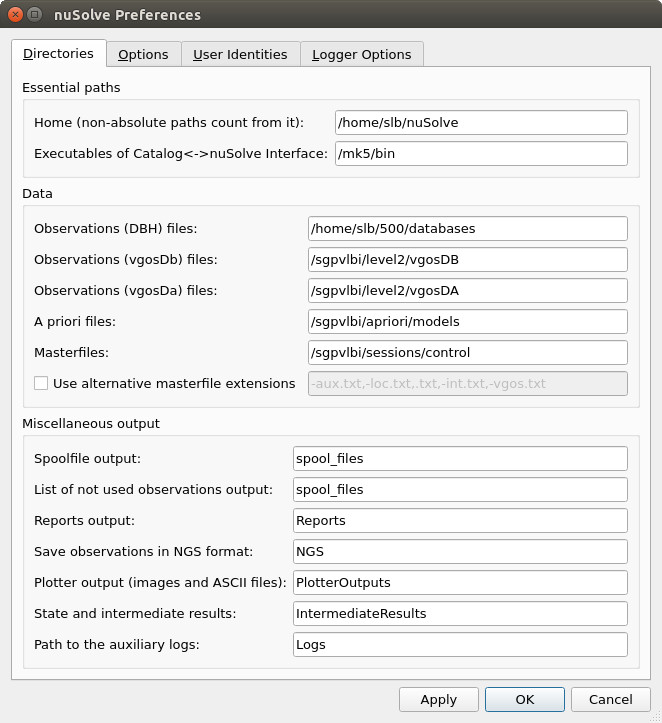
\includegraphics[width=0.6\textwidth]{pref-dirs.jpg}
  \end{center}
  \caption{GUI to set up paths and file names.}
  \label{fig-pref-dirs}
%\end{wrapfigure}
\end{figure}


The path to files in the database handler format (DBH) is given in the
field {\sl Observations (DBH) files}. The field {\sl Observations
(vgosDb) files} displays the path to files with observations in the
new VLBI data format, vgosDb. Files in vgosDa (also known as AGV) format
are in a directory {\sl Observations (vgosDa) files}.

\nuSolve{} can work with files in DBH
format in two modes. One mode, standalone, assumes that  CALC/SOLVE
software is not installed, or the results of data processing will not be
used in CALC/SOLVE. In this case it opens user specified files and saves
results in the same directory in a file with a similar name, but with
the increased version number. In the second mode, interaction with
CALC/SOLVE catalog subsystem, it calls the executable {\tt
catnu\_find\_db} of CALC/SOLVE to inquire about a user-specified
database name. After processing the database is stored with the increased
version number, and the CALC/SOLVE catalog is informed about the new
file by calling {\tt catnu\_update\_cat} executable.

The field {\sl A Priori files} specifies where to look for files with
alternate {\it a~priori} information about site positions, source
coordinates, antenna axis offsets, etc. All this files are in CALC/SOLVE
format. You can ignore this if CALC/SOLVE is not installed.

The directory which contains the masterfiles is pointed to by {\sl
Masterfiles} field. Masterfiles are contain information about VLBI
session and are necessary to produce correct output. There is one
masterfile for each year. You can download the masterfiles from
\begin{center}
{\tt

https://cddis.nasa.gov/archive/vlbi/ivscontrol/

}
\end{center}
\noindent
The masterfiles are updated if the VLBI master schedule changes and you
should periodical get the latest versions. In addition to the standard master
files, a user can use its own "local" master file. The format of the local master
file should be the same as the standard one, its name have to be in the form
"masterYY-loc.txt", where "YY" -- two digits of the year. This feature is designed
for testing purposes or processing non-standard VLBI sessions. The software first
checks for the local master files, if it found a record there it stops the search,
so records in the canonical master files can be overwritten using the local
master file.

Starting with version 0.8.2 of the distribution, an option to expilictly set names
for master files is added. If a user sets the check box {\sl Use alternative
masterfile extensions} to "on", then nuSolve will compose the masterfile names
using a provided list of extensions. The list is a set of strings separated by
comma (","), colon (":") or semicolon (";") char. The software adds the extension
from the list to the basic name, "masterYY" or "masterYYYY", and reads such a file.
The order of files lookup is corresponding to the order of masterfile
extensions in the list. The default list of masterfile extensions is
"-loc.txt,.txt,-int.txt,-vgos.txt".


The directory in the field {\sl Spoolfile output} is used to store a
report about results of data processing in CALC/SOLVE spoolfile format.
The file name is <<SPLF??>> where the last two chars are user's initials
(see the next section). This file is used in routine data processing
by other parts of CALC/SOLVE system.

The field {\sl List of not used observations output} specifies a place
where \nuSolve{} will put a file with a list of observations that are not
in a solution. The list is created at the same time when the report in a
spoolfile format is written. The file name has a form of
<<nuSolve\_unused\_observations\_??>> where the last two chars are user's
initials.

If a user desires, a copy of the spoolfile may also be be saved in the
directory pointed by the field {\sl Reports output}. (See {\sl Copy
spoolfile reports into "Report" directory} on the next tab.) In this case a file
name will be altered from the general <<SPLF??>> to the form of
<<[database name].SFF>>, e.g., {\sl 13SEP12XE.SFF}.

The software \nuSolve{} can export a VLBI session in the ASCII NGS
format. The field {\sl Save observations in NGS format} points to the
directory to put the this output.

The plotting subsystem can save data as ASCII files or graphics (in PS
or PDF format). All output will go into a directory specified in the
{\sl Plotter output (PS, PDF or ASCII files)} field.

The field {\sl State and intermediate results} specifies a path to
files with saved intermediate results, editings and sets of parameters.

When software is invoked in the command line mode, it, in addition to
the standard log file, can save logging information into a separate
for each session file. The field {\sl Path to the auxiliary logs}
points to the directory with such logs.



\subsection{Software options}
\label{prefs-options}
The tab {\sl Options} contains the following selections
(Fig.~\ref{fig-pref-options}).

If the checkbox {\sl Database operations are going through the
catalog} is <<on>>, \nuSolve{} will use the CALC/SOLVE catalog
subsystem.

The option {\sl Saving a database with alternate session code (for
tests purposes)} is used for tests. If it is <<on>> the name of the
database will be altered so it will be possible to have different
solutions for comparisons.

If the option {\sl Copy spoolfile reports into "Report" directory} is
selected, \nuSolve{} will make a copy of the report in spoolfile format
as a separate file (see above).

\begin{figure}[htb!]
\begin{center}
    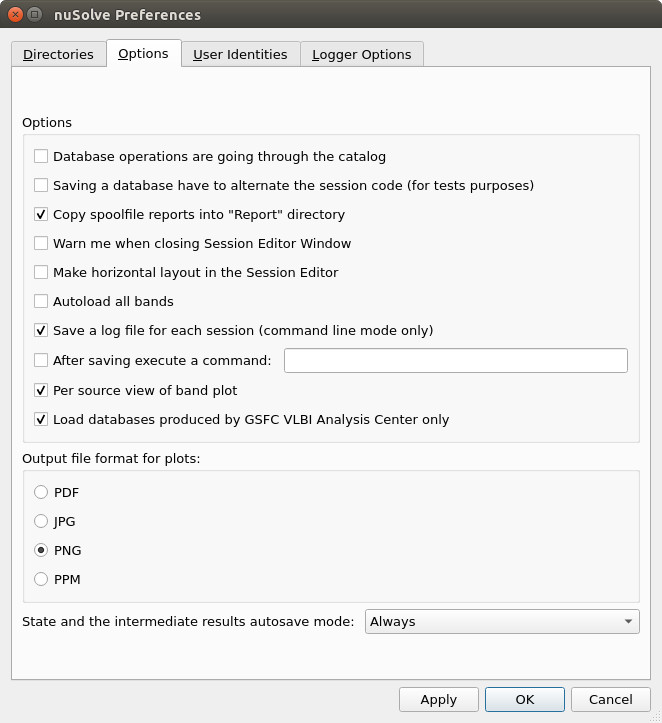
\includegraphics[width=0.6\textwidth]{pref-opts.jpg}
\end{center}
\caption{GUI to set up \nuSolve{}'s options.}
\label{fig-pref-options}
\end{figure}

The checkbox {\sl Warn me when closing Session Editor Window} switch
<<on/off>> determines if \nuSolve{} will issue a warning when a user
closes the Session Editor Window. This is because a click on {\sl Close}
button of the window would destroy your work if you are not done with
your analysis.

For some displays with small resolution the Session Editor window will
not fit on the screen. In this case turn the {\sl Make horizontal
layout in the Session Editor} checkbox <<on>>. It will put a series of
buttons on the right instead of bottom of the window. The software is
still in developmental mode and in future releases we will redesign the
window to overcome this problem.

In general, when a user specifies a file name with a database,
\nuSolve{} automatically looks for files of the session with other bands
and reads them too. E.g., if a user asks to open {\sl 13SEP12XE} file,
it will pick up {\sl 13SEP12SE} too (if it exists). To override this
behavior uncheck the {\sl Autoload all bands} checkbox. If this box is
not checked only one file will be opened.

Running in the command line mode the software will save per session log
files if the checkbox {\sl Save a log file for each session (command
line mode only)} is set to <<on>>, otherwise the logging information
will be lost.

If the checkbox {\sl After saving execute a command} is set to <<on>>,
\nuSolve{} will run a command that is specified in the next field every
time when it saves a session in a new database or vgosDb files.
The command can be either a binary executable or a script, it have to
be in the user's PATH or a full path have to be provided. Five arguments
are passed to the command: a database name, an official session code
and name (the both fields are from a masterfile), network ID and user's
initials. For example, assume I have a script {\sl testExternalCommand}
in a place that is listed in my {\sl \$PATH} environmental variable and
the script consists of a simple instruction
\begin{verbatim}
#!/bin/bash
echo $1 $2 $3 $4 $5
\end{verbatim}
\noindent
Then, when I have processed a session {\sl \$17FEB23XE} and pressed
{\sl Save} button the following string will also be sent to the standard
output:
\begin{verbatim}
$17FEB23XE R4780 IVS-R4780 IVS-R4 SB
\end{verbatim}

The checkbox {\sl Per source view of band plot} controls an option
to plot data for a selected (or a set of selected) source on the Band/Data
plot of the session editor. If the check box is <<on>>, a listview with
names of sources will appear next to the plot, a user can select sources
for which data should be displayed. However, for displays with small
resolution all elements of the session editor window could not fit to
a screen, in such case a user can turn off the checkbox.

When a user loads a vgosDb database providing a session name, nuSolve
usually reads the lates version of a wrapper file of the database.
However, sometimes it is preferrable to load the latest version produced
by your analysis center even if a higher version created by another
institution already exists. In this case turn on the checkbox
{\sl Load databases produced by [local] VLBI Analysis Center only}, where
[local] is an abbreviated acronym of your analysis center (see subsection
\emph{\ref{prefs-uids} User's identities}}).


The option {\sl Output file format for plots} tells \nuSolve{} in
what format plots should be saved. Currently, the following formats
are supported: PDF (vector) format and JPG, PNG, PPM (raster) formats.


And the last option, {\sl State and intermediate results autosave
mode}, specifies how frequently a procedure of autosaving have to be
performed. There are three modes, {\sl None}, {\sl On Exit} and {\sl
Always}. The procedure stores the intermediate results and the
parameterization in a separate file in the corresponding directory.


\subsection{User's identities}
\label{prefs-uids}
To generate proper report files and reflect history of changes in the
data files, a user has to provide the corresponding information. It is
collected in the {\sl User Identities} tab of the {\sl Preferences}
window, Fig.~\ref{fig-pref-uids}.

If you make data processing and submit your results to the IVS, you have
to provide correct information in the files.

There are two groups, {\sl User} and {\sl Analysis Center}, that
contain fields that describe a user and an analysis center.

\begin{figure}[htb!]
%\begin{wrapfigure}{l}{0.5\textwidth}
\begin{center}
    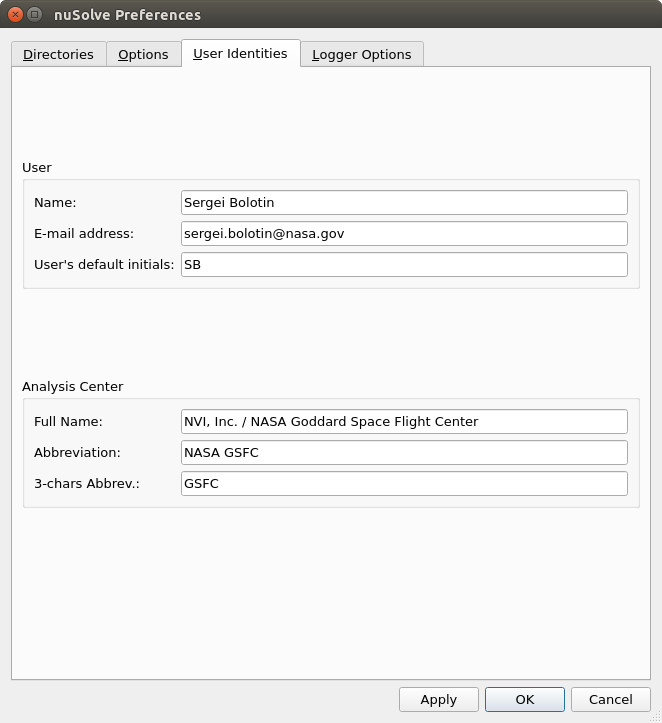
\includegraphics[width=0.6\textwidth]{pref-uids.jpg}
\end{center}
\caption{GUI to set up identities of an analysis center and a user.}
\label{fig-pref-uids}
\end{figure}
%\end{wrapfigure}

The first group has full user name, user's e-mail address and initials.
The name and the e-mail address will appear in the report in spool file
format. The two-letter initials are the 'solve-initials', and
historically are appended to a prefix {\sl SPLF} to generate the
spoolfile name, e.g., {\sl SPLFSB} in the case as shown on the figure.

The second group contains full name of analysis center, its abbreviated
form and a few-letters abbreviated acronym. The latest attribute for your
analysis center can be found at
\begin{center}
{\tt
https://cddis.nasa.gov/archive/vlbi/ivscontrol/ac-codes.txt
}
\end{center}
\noindent
If your analysis center does not have a three-letter code and you are
going to participate in IVS activities, please contact {\tt
mail-to:ivscc@ivscc.gsfc.nasa.gov} to request the code.


\subsection{Configuration of logging subsystem}
\label{prefs-options-logger}
The last tab, {\sl Logger Options}, controls the logger behavior. All
parts of the software communicate with a user through {\it logger}. The
logger is a small object that accepts messages from other parts of the
software and prints them on the main (=log) screen. Depending on log
facility and log level a message will or will not appear on the log
screen.

The group {\sl Logger's Options} specifies a file name of the log
output ({\sl Log file name}), number of lines that will be kept on the
screen ({\sl Log capacity}), whether the log outputs should be saved
at all ({\sl Save log to the file}) and if it is desired to add a time
stamp to the message ({\sl Put time stamps}). If you want in addition
to time stamp add a date too, set the checkbox {\sl Use full date format}
to <<on>>.

{\bf \color{red}WARNING}: If the logger is instructed to save data in
the log file, the size of the file will grow up. \nuSolve{} does not
check the size of the file (it does not know about your intentions), and
eventually the file could take all free space on your computer! If you
do not need the log output from previous runs, please, remove the file on
a regular basis.

\begin{figure}[htb!]
%\begin{wrapfigure}{l}{0.5\textwidth}
\begin{center}
    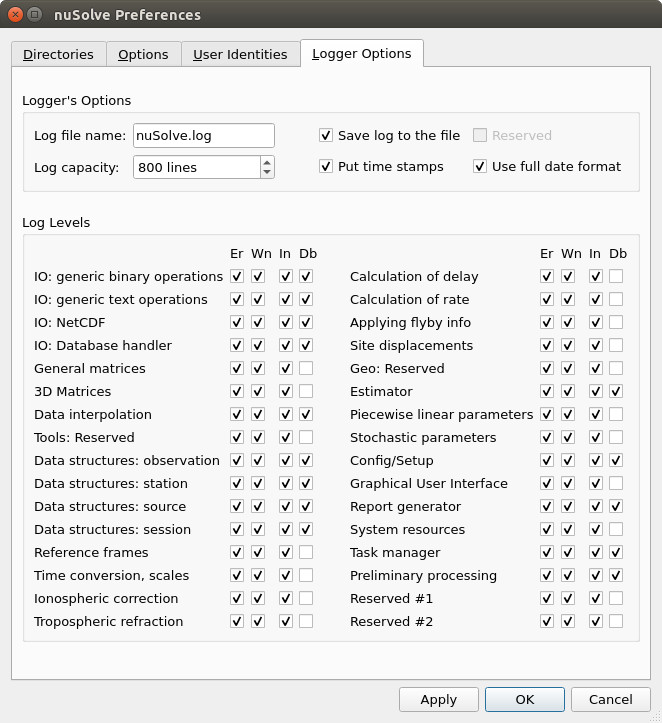
\includegraphics[width=0.6\textwidth]{pref-logs.jpg}
\end{center}
\caption{GUI to set up logger options.}
\label{fig-pref-logger}
\end{figure}

Currently, there are four log levels: error, warning, informational and
debug. Error messages are generated when something wrong happens and
\nuSolve{}'s behavior is unstable or unpredictable. Examples include
missing essential files (e.g., file with VLBI observations), or an
inconsistency in the data. Warnings are issued if something unexpected
happened but the software is able to deal with it. For example, if a
VLBI station that participates in the session was not found in the file
with the external {\it a~priori} coordinates. In this case \nuSolve{}
will use coordinates from the database as {\it a~priori}, and it notify
the user about this issue. The last two log levels, informational and debug,
are interesting mostly for developers.

In the group {\sl Log Levels} one can find a table of log levels ({\sl
Er} -- error, {\sl Wn} -- warning, {\sl In} -- informational and
{\sl Db} -- debug) and facilities. The log facility is an integral
part of the software that generates the message and most routines use
this facility. Two examples are the graphical user interface or
evaluation of ionospheric correction. Separation of logging output by
levels and facilities allows developers to focus on some particular
topic without altering other parts of the software.



%%%%%%%%%%%%%%%%%%%%%%%%%%%%%%%%%%%%%%%%%%%%%%%%%%%%%%%%%%%%%%%%%%%%%%%%%%%%
%%
%%
%%
%%%%%%%%%%%%%%%%%%%%%%%%%%%%%%%%%%%%%%%%%%%%%%%%%%%%%%%%%%%%%%%%%%%%%%%%%%%%
\section{Configurations of data analysis process}
\label{sect-config}

The second set of options, configuration, is more VLBI-centric. To get an
access to the configuration, select menu {\sl Edit-->Edit General Config}
or press {\sl Ctrl+g} keys.
A dialog window that allows to change the options will appear on the
screen. A similar widgets will be available on Session Editor window too
with some exceptions. Some of these options specify what and how
software have to act when it reads a VLBI session, these options will
not be available on Session Editor window.


\subsection{General options}
\label{sect-config-general}
The first tab of General Configure Editor window, {\sl General}, shows
general options (Fig.~\ref{fig-options-general}).

The groups {\sl Delay type} and {\sl Rate type} allow a user to switch
between the types of observables. Currently, \nuSolve{} process single
band delays, group delays, phase delays and delay rates. The use of the
last two types, phase delays and delay rates, is in a preliminary stage
and should be used for testing purposes mostly.


\begin{figure}[htb!]
%\begin{wrapfigure}{l}{0.5\textwidth}
\begin{center}
    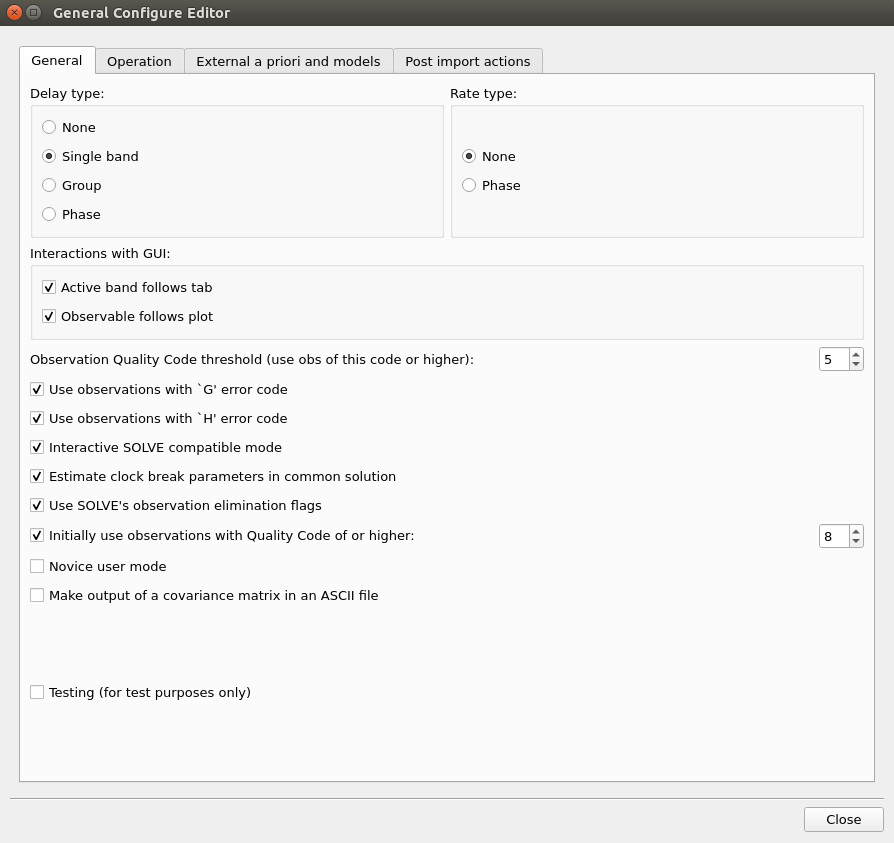
\includegraphics[width=0.6\textwidth]{options-general.jpg}
  \end{center}
  \caption{Configuration: general options.}
  \label{fig-options-general}
\end{figure}


Another widget group, {\sl Bands}, will appear on Session Edit window
(see Section~\ref{subsect-sessedit-options}).
It will display available for a particular session bands and allows
a user to select an active band.

However, in practice it is not convenient to go every time to the tab
{\sl Options} of the Session Edit window and change the current
observable or the active band manually. \nuSolve{} can do it
automatically depending on what the user is looking at. If the check box
{\sl Active band follows tab} of the group {\sl Interactions with GUI} is
checked, then the active band will always be the band which is currently
visible on the tab {\sl Bands}. If the check box {\sl Observable follows
plot} is checked and the delay rates are not in a solution, then when a
user selects single band delay residuals as the Y-axis of the plot on the
tab {\sl Bands}, \nuSolve{} will automatically set the observable to
single band delays. The same is true for the group or phase delays. If a
user chooses any other column as the Y-axis of the plot, the previously
selected observable will not change. If delay rates are in the solution
(i.e., {\sl Rate types} are not {\sl None}), the feature of the automatic
switching of the observables is suppressed. These two check boxes are
checked by default.

The software does not include in data analysis the observations with low
quality code. The spin box {\sl Observation Quality Code threshold (use
obs of this code or higher)} specifies this threshold.

The check box {\sl Interactive SOLVE compatible} assures that all
calculations are done in interactive SOLVE compatible mode. It is recommended
to turn this mode on.

The next check box {\sl Estimate clock break parameters in common solution}
switches a mode of treating the clock breaks. If the checkbox is <<on>>,
\nuSolve{} will estimate parameters of clock break(s) in a common solution
(as interactive SOLVE does). If the checkbox is <<off>>, the parameters of
clock break(s) are estimated once and then are applied as a step wise
function to the clocks of a station.

To take into account stored in a database observation elimination flag
keep the check box {\sl Use SOLVE's observation elimination flag}
turned on.

There is also an option to use observations only with definitely good
quality codes and then later, at the stage of outlier restoration, to
add all other observations with all acceptable quality codes. This
option mimics interactive SOLVE and can be modified with {\sl Initially
use observations with Quality Code of or higher} check box and the
associated spin box.

The {\sl Novice user mode} check box turns on <<Novice user>> mode.
The difference of the mode and the normal operation is in verification
of the "accomplishments" that were done for the session before exporting
data. Currently, if the mode is <<on>> the software checks for existence
of the ionosphere corrections and reweighting before save a session.
If these operations were not performed, a warning message will be issued.
A user can override the warning answering {\sl Yes}. Also, a warning
message will occur if a user will try to calculate ionosphere corrections
before resolving group delay ambiguities or attempt to resolve the
ambiguities if the the ionosphere corrections are already evaluated.

If the checkbox {\sl Make output of a covariance matrix in an ASCII file}
is <<on>>, a covariation matrix will be stored in the directory with
spool file output in an ASCII file <<PALL??>> with the last two characters
of user initials.

The check box {\sl Testing (for debug purposes only)} is designed to
turn on some part of code that performs a debug procedure. Do not use
this feature unless you are intending to debug the source codes.


\subsection{Run time options}
\label{sect-config-runtime}

This tab, {\sl Operation} collects options that are most demanding
during data analysis, Fig.~\ref{fig-options-operations}.

\begin{figure}[htb!]
%\begin{wrapfigure}{l}{0.5\textwidth}
\begin{center}
    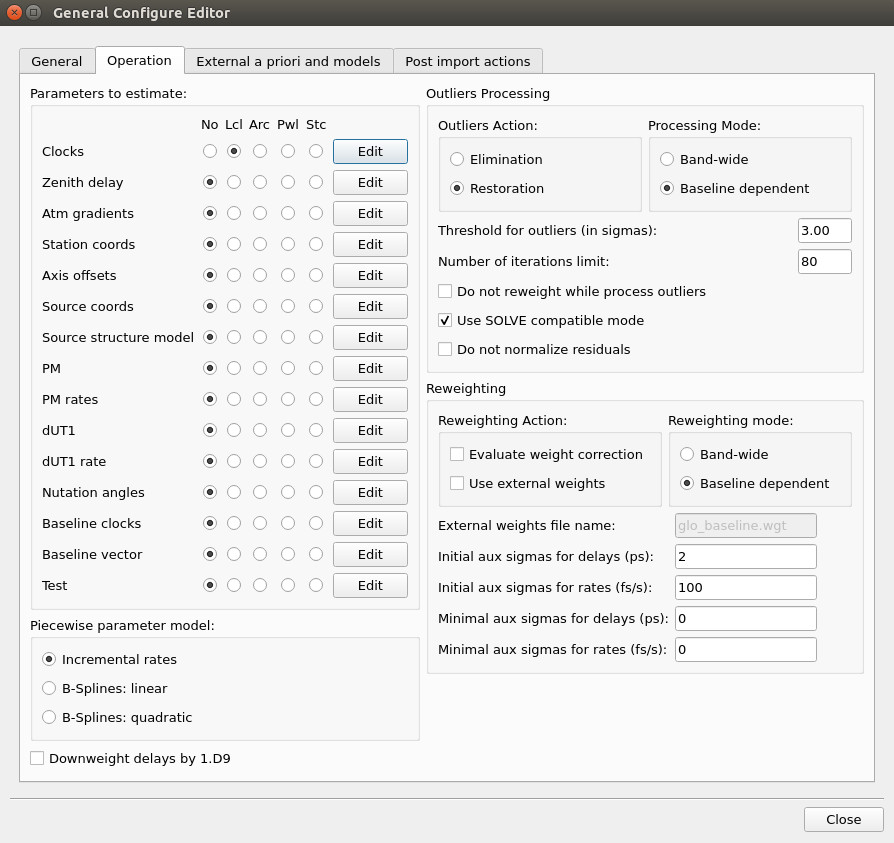
\includegraphics[width=0.6\textwidth]{options-operations.jpg}
  \end{center}
  \caption{Configuration: operational options.}
  \label{fig-options-operations}
\end{figure}

The first group, {\sl Parameters to Estimate}, specifies the parameters
that will be estimated during data processing. The group consists of a
table with the parameter names in the first column. The next five
columns of radio buttons specify the type of parameter. The first type,
{\sl No} means "do not estimate a parameter". The type {\sl Lcl}
specifies estimation of the parameter based on the whole set of
observations of the session. The type {\sl Arc} treats a parameter as
an arc parameter, where unbiased estimates of the parameter are made for
user specified time intervals that are smaller than a whole session
length. Usually, the lengths of arcs are 1, 2 or 3 hours. A user can
change the arc length for the parameter by pressing the {\sl Edit}
button in the last column (see Fig~\ref{fig-sessedit-options-pe}). The
next type, {\sl Pwl}, treats a parameter as a piecewise-continuous
function. It is similar to the arc type but the model requires the
parameter to be continuous. There are three models implemented in
\nuSolve{} to deal with piecewise-continuous parameters. Two of them,
incremental rates and linear B-Splines, came from CALC/SOLVE. The
third model is quadratic B-Splines.

A user can change the mode of PWL parameters in the group {\sl
Piecewise-continuous parameter model} just below the {\sl Parameters to
Estimate} group. The realization with B-splines needs much less CPU
time while the incremental rates mode produces results that are same as
obtained with interactive SOLVE. The last parameter type is a stochastic
parameter, given in the last column, {\sl Stc}. Currently, the
2$^{nd}$ order Markov process and its two extreme cases, white noise and
random walk, are realized in \nuSolve{}. Modeling a time varying
parameter as a stochastic parameter has some restrictions; this type
cannot be combined with arc or PWL. Do not mix these types in a solution
as the results will be unpredictable.

The checkbox {\sl Downweight delays by 1.D9} turns on "downweighting" of
the delays. When delays and delay rates are processed in one solution
and this checkbox is turned <<on>>, then effective standard deviations
of delays are multiplied by $10^{4}$ to reduce the influence of the
delays in the solution. This option is taken from interactive SOLVE.


\begin{figure}[htb!]
  \begin{center}
    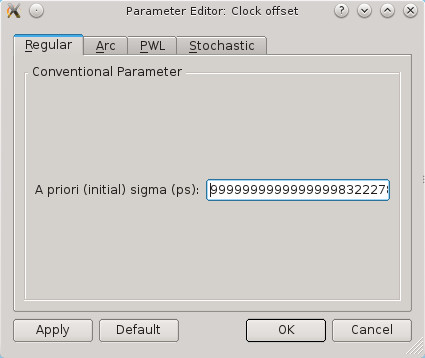
\includegraphics[width=0.22\textwidth]{sessedit-options-pe-loc.jpg} \hspace{2mm}
    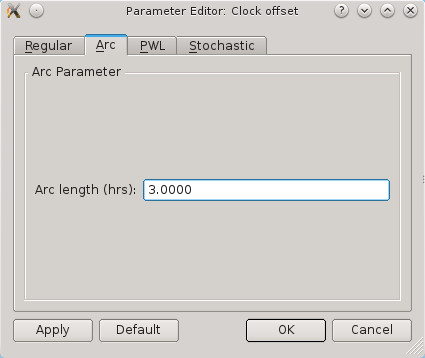
\includegraphics[width=0.22\textwidth]{sessedit-options-pe-arc.jpg} \hspace{2mm}
    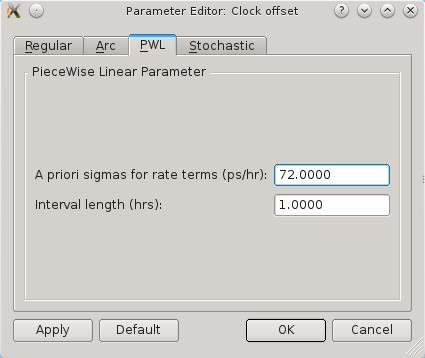
\includegraphics[width=0.22\textwidth]{sessedit-options-pe-pwl.jpg} \hspace{2mm}
    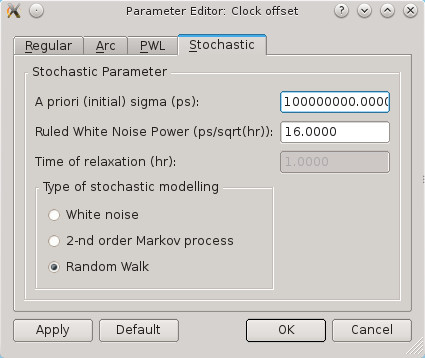
\includegraphics[width=0.22\textwidth]{sessedit-options-pe-stc.jpg}
  \end{center}
  \caption{Parameter options editor: local (leftmost), arc, piecewise and stochastic (right) parameters.}
  \label{fig-sessedit-options-pe}
\end{figure}

The group {\sl Outlier Processing} determines the response of
\nuSolve{} when a user presses the button {\sl Outlr} of the Session
Edit window. If {\sl Outlier Action} is set to {\sl Elimination},
then when the user clicks the button, the software will check the
residuals and mark the outliers that are not to be used in further
solutions. If the type of action is set to {\sl Restoration}, then
previously eliminated observations will be included in next solutions.

The procedure of outlier elimination or restoration is performed in the
following way. Normalized residuals are calculated for a set of
observations determined by the {\sl Processing Mode} setting (for a
whole band, {\sl Band-wide}, or for each baseline, {\sl Baseline
dependent}). Then, an observation with normalized residual greater than
or less than a specified threshold (specified by the {\sl Threshold for
outliers (in sigmas)} line editor) is marked for exclusion or
inclusion. In the elimination process, the software removes the
observation with the largest normalized residual. Then \nuSolve{} makes
an estimate of parameters and recalculates the residuals. The whole
procedure is repeated several times until no observations exceed the
threshold or the number of iterations exceeds the specified user limit,
{\sl Number of iterations limit}. In the restoration process,
observations that were not initially included in the solution (typically
because they had quality codes less than 8-9) are considered for
restoration. The software includes observations of this type with the
smallest normalized residuals as long as their normalized residuals were
less than the specified threshold. Then \nuSolve{} estimates parameters
and recalculates the residuals. The whole procedure is repeated until
all observations of this type have been included. The elimination and
restoration processes are repeated until no observations can be
eliminated or restored. The procedure of outlier elimination is
performed in conjunction with the procedure of weight corrections. To
minimize the time of data processing, weight correction calculations can
be skipped between iterations. This option is controlled by the {\sl
Suppress weight correction in outliers processing} check box. The
check box {\sl Process outliers in the SOLVE compatible mode} assures
that the normalized residuals are evaluated in the same way as
interactive SOLVE does.

The {\sl Reweighting} group controls the process of weight correction.
The weight correction calculations are performed on the fly, after the
user presses the {\sl Process} button, at the stage when new residuals
are available. These calculations are relatively time consuming and by
default they are turned off. Usually, we turn on evaluation of
additional weights after clock breaks are fixed, ambiguities are
resolved, ionospheric corrections are evaluated and large outliers are
removed. The check box {\sl Evaluate weight correction} is responsible
for this. Instead of performing the reweighting computations, it is
possible to use additional weights from an external file in a solution.
This option is implemented mostly for compatibility with interactive
SOLVE and testing purposes. There are two widgets in the {\sl
Reweighting} group: the check box {\sl Use external weights}, which
turns <<on>> or <<off>> the use of the external weights, and the {\sl
External weights file name} line editor, which allows the user to
specify the file. The weight corrections can be evaluated for a whole
set of observations over all baselines, which is the {\sl Band-wide}
mode, or for each baseline separately, which is the {\sl Baseline
dependent mode}. In addition, a user can specify values for initial
additional weights (for delays and rates) and for minimal values of
these parameters.



\subsection{Applying different models and using external a priori information}
\label{sect-config-models}

The third tab, {\sl External a priori and models}, specifies how
the software will apply different available models and use {\it a priori}
information from external files. This tab is shown on Fig.~\ref{fig-options-models}.

\begin{figure}[htb!]
%\begin{wrapfigure}{l}{0.5\textwidth}
\begin{center}
    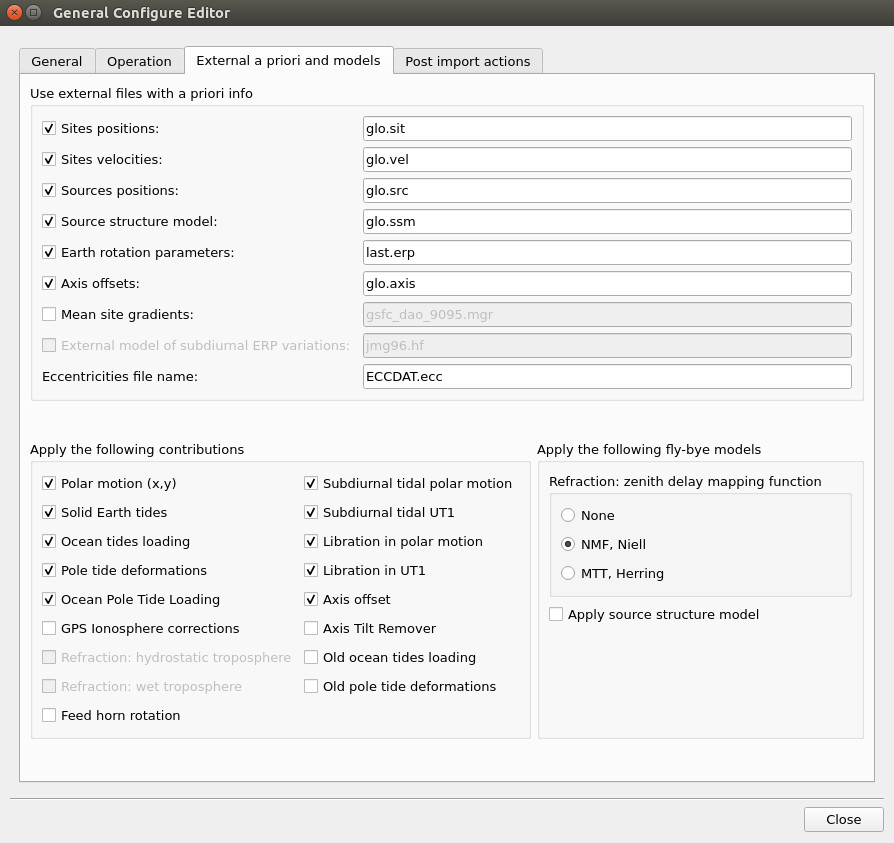
\includegraphics[width=0.6\textwidth]{options-models.jpg}
  \end{center}
  \caption{Configuration: use of contributions and external {\it a priori} information.}
  \label{fig-options-models}
\end{figure}


The group {\sl Use external files with a priori info} allows a user to
use {\it a~priori} values of various parameters from external files. In
general, the theoretical values and partial derivatives of observables
with respect to parameters are evaluated by CALC software and stored in
databases. The {\it a~priori} which were applied in these
calculations are also stored in the database. Sometimes it is convenient
to use {\it a~priori} values that are different from the initial
ones. For example, suppose a station has moved due to an earthquake but
CALC used station positions from an ITRF solution. In this case the
actual station position will differ from the {\it a~priori} position and
this difference will cause an increase of residuals. Depending on the
shift, the large residuals will make it impossible to resolve
ambiguities (at the S-band especially) correctly and to eliminate
outliers. Another case when we need external {\it a~priori} values is
when observations of new sources are included in VLBI analysis. Prior
to analysis of the first few sessions with a new source, it is
impossible to determine its coordinates with the necessary precision
without using an approximate external {\it a~priori} position.

All files but one mentioned in the widget group are ASCII files in the format that
is used by CALC/SOLVE. If CALC/SOLVE is not installed on your computer
and the user wants to apply external {\it a~priori} values, he/she
should get the corresponding file(s) from somewhere else or consult the
source codes. The files are expected to be in the directory specified in
{\sl References} by {\sl A Priori files} field. However, a user can
overwrite this assumption specifying an absolute path there.
The {\sl Site Positions} and {\sl Site Velocities} check boxes turn
<<on>> or <<off>> using the external {\it a~priori} for the
corresponding parameters. The file names are entered in the
corresponding line editor box.
The check box {\sl Source Positions}
controls using external {\it a~priori} values for sources coordinates.
The {\sl Source structure model} check box specifies an external file
with parameters of source structure models
see section \emph{\ref{section-using-gui-ssm} Using a source structure model} for details.

The checkbox {\sl Earth rotation parameters} refers to polar motion
($p_x$, $p_y$) and Earth rotation $d(UTC-UT1)$. The software can read
files of three types: the Earth rotation parameters (polar motion and
dU1) in "ERP" file format (generated by eopkal utility from CALC/SOLVE
package), the Earth orientation parameters (ERP plus the nutation angles)
generated by USNO and IERS. The EOP files from USNO should be available
at
\begin{center}
{\tt
https://www.usno.navy.mil/USNO/earth-orientation/eo-products/weekly
}
\end{center}
\noindent
and mirrored at
\begin{center}
{\tt
https://cddis.nasa.gov/archive/products/iers
}
\end{center}
\noindent
The file is called <<finals2000A.data>>. The IERS EOP file(s) is available
at
\begin{center}
{\tt
https://www.iers.org/IERS/EN/DataProducts/EarthOrientationData/eop.html
}
\end{center}
\noindent
it is called <<EOP\_14\_C04\_IAU2000A\_one\_file\_1962-now.txt>>. All three
types of files are ASCII files and do not contain marks to identify
the type of a file. The software assumes that file extension <<.erp>>
specifies "ERP" format (output of eopkal), the extension ".data" means
USNO generated EOP files and the extension ".txt" is for EOP IERS C04
solution. Using external a priori EOP files from USNO and IERS is in
testing mode. Unfortunately, EOP from both institutions have nutation
angles that are not smoothed. That make them useless in interpolation.
Though, it should be ok to use such files for processing a new INT session,
when the nutation angles are derived not from VLBI observations, but is
a prediction.


{\sl Axis Offsets} and
{\sl Mean Site Gradients} are self explanatory. The check box {\sl
External model of subdiurnal ERP variations} specifies the use of an
external model of the diurnal and semidiurnal oscillations of Earth
rotation parameters. If the check box is <<on>>, \nuSolve{} will apply
the external model of subdiurnal ERP variations entered in the line
editor box.
The last row of the widgets group allows a user to specify a file with
stations eccentricities.

The next group, {\sl Apply the following contributions}, specifies
which effects should be used in data analysis. By {\it contribution} we
mean the impact of some geophysical effect on the predicted values of
observables. The CALC software evaluates delays and delay rates by
applying some standard models. Other standard models are also evaluated
and stored in the database, but are not added to the precalculated
values. Moreover, some alternative models are evaluated and stored in
the database. CALC/SOLVE (and \nuSolve{}) takes into account a model by
adding the corresponding contribution. To apply an alternative model,
the applied contribution should be subtracted and an alternative
contribution added to precalculated observables. Some of contributions
listed in {\sl Apply the following contributions} are necessary to
obtain a solution, e.g., polar motion or solid Earth tides. Others are
required to get a <<standard>> solution. Few contributions are added
for testing purposes or should be used in rare cases. One of the contributions,
{\sl GPS Ionosphere corrections} is provided by external software.
The list of available contributions is determined by current version of CALC.
Two checkboxes, {\sl Refraction: hydrostatic atmosphere} and
{\sl Refraction: wet atmosphere}, works in a different way: if a
checkbox is turned <<on>>, then the contribution stored in a database
will be used. If the checkbox is set to <<off>>, the corresponding
values will be calculated by the software on fly.

The widget group {\sl Apply the following fly-by models} allows to a
user to control models that will be calculated by \nuSolve{} and applied
during analysis of observations (on the fly). A user can specify
what zenith delay mapping function should be used: NMF \cite{Niell1996}
or MTT \cite{Herring1992}. To use or not a model of source structure
effect is controlled by a check box {\sl Apply source structure effect}.
For the source structure effect a particular source should have parameters
of the model in the corresponding external file (see above) and the
source needs to be configured to use the model (see below, subsection
\emph{\ref{subsect-sessedit-sources-list} Tab <<Sources (List)>>}).


\subsection{Configuring post import actions}
\label{subsect-config-pia}

The rightmost tab, {\sl Post import actions}, specifies what
procedures should be called after successful reading of a VLBI session.
Configuration of the procedures are network dependent. The software
separates all existing VLBI sessions by <<network>> type. For each type
of network a user can set up its individual configuration. \nuSolve{}
determines the network type of a session by consulting an appropriate
masterfile. If \nuSolve{} is unable to determine the network type of a
session, it will use {\sl DEFAULT} set up, as it shown on
Fig.~\ref{fig-options-pia}. Also, if a configuration for the network
type of the session was not set, the {\sl DEFAULT} set up will be
used. Currently, the set of network types and theirs attributes are
hard coded into the software and cannot be modified by a user.

\begin{figure}[htb!]
%\begin{wrapfigure}{l}{0.5\textwidth}
\begin{center}
    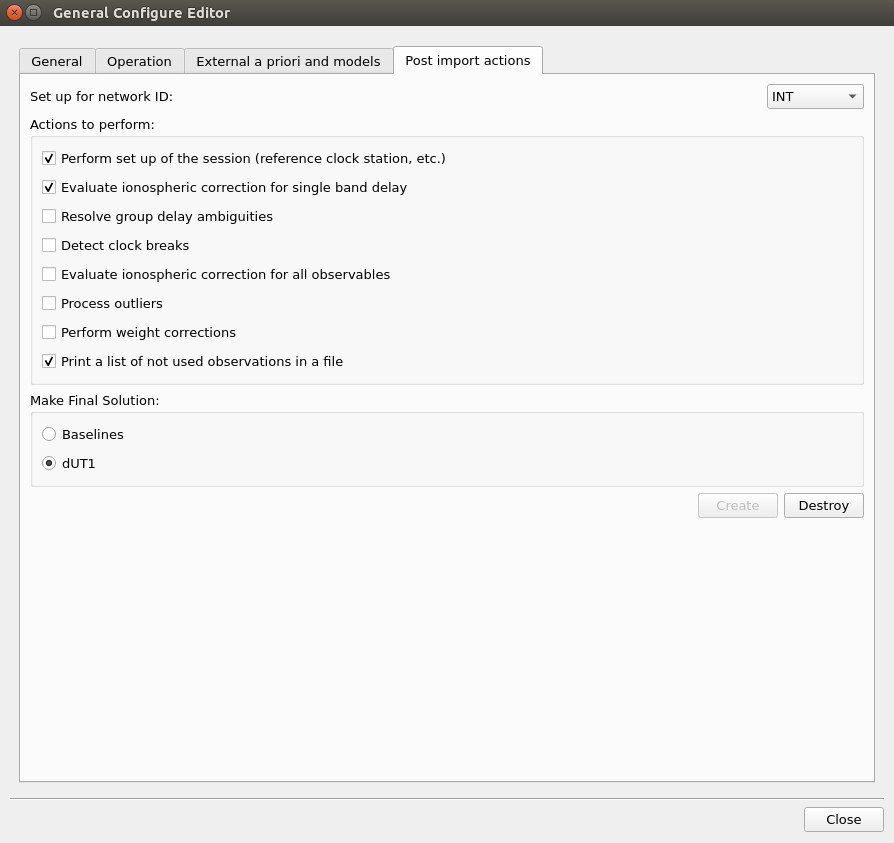
\includegraphics[width=0.6\textwidth]{options-pia.jpg}
  \end{center}
  \caption{Configuration: set up of post import actions.}
  \label{fig-options-pia}
\end{figure}

To select a type of a VLBI network, click on a combobox labeled {\sl
Set up for network ID}. All available VLBI network names will appear
in a list of the combobox.

The checkboxes in the widget group {\sl Actions to perform} specify
what procedures will be automatically called after a session has been read.

The first action, {\sl Perform set up of the session}, assigns a
reference clocks status to one of the stations, turns off a <<estimation
of station positions>> flag for one of the stations (by default this
flag is <<on>> for all stations) and checks the history part of a
database trying to figure out for which station manual phase calibrations
were applied and, if found, turns the attribute {\sl use cable calibration}
<<off>> for such station.

The second action performs calculation of ionospheric corrections for
the single band delays only.

The first two post-import actions are useful for data analysis of practically
any session, therefore they are turned <<on>> for {\sl DEFAULT} set up.

The rest of actions are designed for automatic process of intensive sessions
(e.g., IVS-INT1, IVS-INT2, IVS-INT3). We do not recommend use them for other
type of VLBI sessions. These actions are self explanatory.

The last action, {\sl Print a list of not used observations in a file}, toggles
creation of a file with a list of all observations that are not in the
last solution. The file has a name <<nuSolve\_unused\_observations\_??>>
where the last two chars are user's initials, it is placed in a directory
specified in software Preferences (see Subsection~\ref{prefs-general}).


The group {\sl Make Final Solution} allows a user to select which type
of solution should be used for evaluation of weight corrections. The
standard practice for processing intensive sessions is to estimate clock
parameters and zenith delays of observing stations and changes of Earth
rotation, $d(UT1-UTC)$. However, there are cases when either Earth
orientation parameters are not known correctly or {\it a priori} station
positions differ form the actual ones. In these cases it is possible to
estimate baseline vectors instead of $d(UT1-UTC)$. This type of solution
will absorb deviances of {\it a priori} EOP or station positions so it
will make possible to deselect outliers and evaluate realistic weight
corrections.

The software does not keep configurations for all networks. In the beginning,
there are two sets of configurations, one is for {\sl INT} sessions and
another one is {\sl DEFAULT}. A user can add a set up for some particular
VLBI network by choosing the network in the combobox {\sl Set up for network
ID} and then clicking a button {\sl Create}. After that, when a
configuration has been created, a user is able to modify the actions.
To delete existing set up, press a button {\sl Destroy}. The {\sl DEFAULT}
configuration is not possible to delete.



%
%%%%%%%%%%%%%%%%%%%%%%%%%%%%%%%%%%%%%%%%%%%%%%%%%%%%%%%%%%%%%%%%%%%%%%%%%%%%%%
%
%
\chapter{Plotting subsystem}

To visualize and edit sets of data we developed a small and simple
plotting subsystem (or plotter). Since the plotter appears in various
parts of data analysis procedure and has the same controls, we discuss
it in this separate section.

\begin{figure}[htb!]
%\begin{wrapfigure}{l}{0.5\textwidth}
\begin{center}
    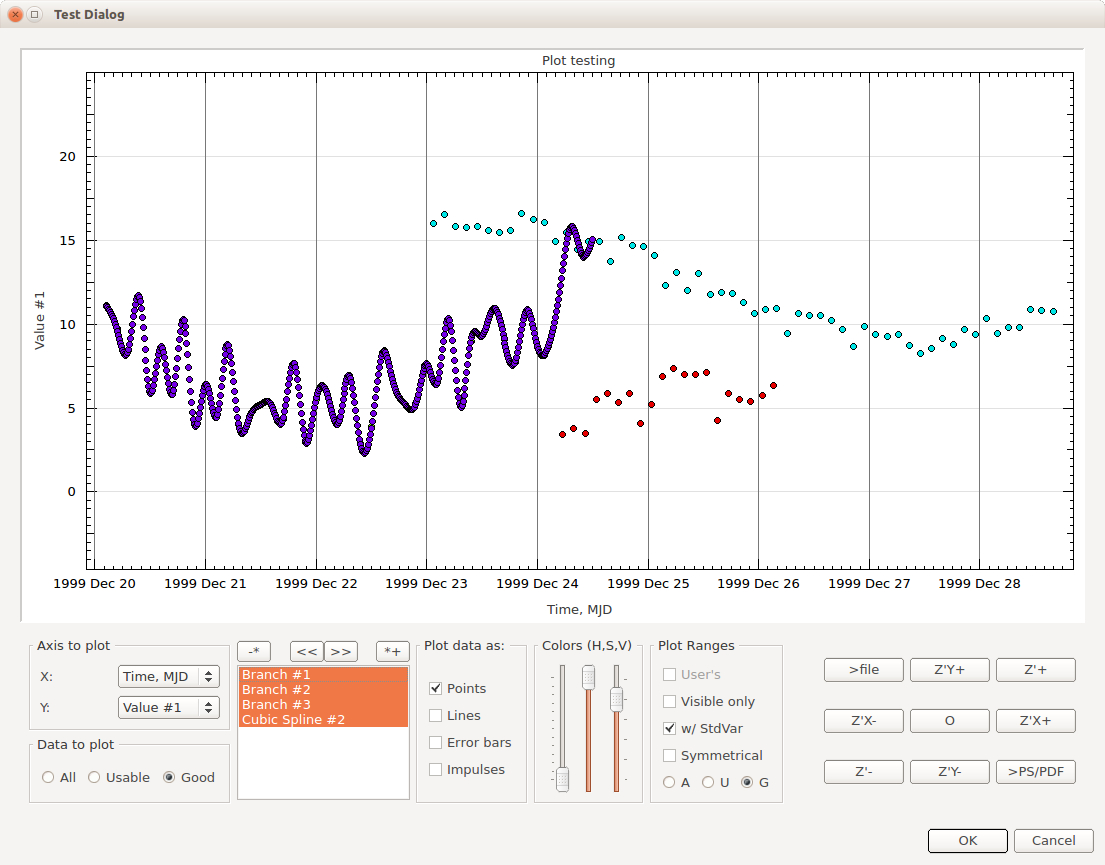
\includegraphics[width=1.0\textwidth]{plotter-general.jpg}
  \end{center}
  \caption{Test plot.}
  \label{fig-plot-general}
\end{figure}

The plotter (Fig.~\ref{fig-plot-general}) consists of a canvas, where
the data are plotted, and controls, that are widgets that allow a user
to modify how and what part of data will be plotted. In addition, a user
can interact with the canvas too to make selections or deselections and
get information about the data. Also, the plotter emits signals as a
reaction to the user pressing keys, so it is possible to plug in
external functionality.

In general, the plotter accepts multiple sets of data in the same
format. Each set of data (called here {\it branch}) is plotted with the
same color. If the user decides to make a plot with connected lines,
points of each branch will be linked separately. Each point on the canvas is
represented by a vector of dimension 2 or higher. Each element in the
vector is considered as having the same property (physical meaning,
units, etc.) for all points. For examples, one vector could consist of
delay and sigma. Not all data is expected to have corresponding sigmas.
Some of elements can be assigned a special property and will have
special treatment. E.g., if the software sets a Type\_MJD attribute,
then the plotter will treat that data as time in MJD scale and put
proper labels (if this element is set to be the x-coordinate).

The current distribution of \nuSolve{} has the ability to test the
plotting subsystem. Select menu {\sl Test-->Test Plotter} to invoke a
window with some artificial data. On the plot there are four branches
labeled {\sl Branch \#1}, which consists of time-tags, {\sl Branch
\#2}, {\sl Branch \#3} consist of data with corresponding sigmas, and
{\sl Interpolation \#2} is a cubic spline interpolation of {\sl
Branch \#1}.



%%%%%%%%%%%%%%%%%%%%%%%%%%%%%%%%%%%%%%%%%%%%%%%%%%%%%%%%%%%%%%%%%%%%%%%%%%%%
%%
%%
%%
%%%%%%%%%%%%%%%%%%%%%%%%%%%%%%%%%%%%%%%%%%%%%%%%%%%%%%%%%%%%%%%%%%%%%%%%%%%%
\section{Plotter controls}
The plotter controls (Fig.~\ref{fig-plot-controls}) are the following
widgets: selection of axis to plot, list of branches, selection of how
to plot the data (with points, lines, errorbars or impulses (lines from
the X-axis to the point), modifying colors of the branches (hue,
saturation and value), altering ranges on the plot, scaling and output
controls.

\begin{figure}[htb!]
  \begin{center}
    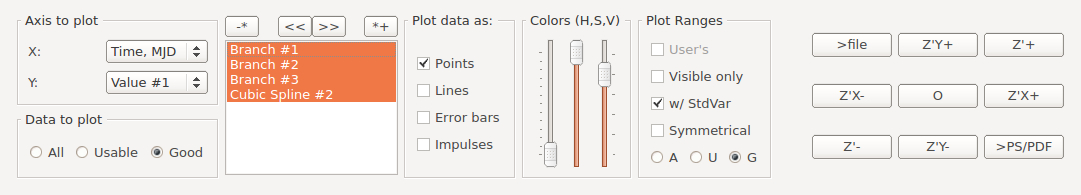
\includegraphics[width=1.0\textwidth]{plotter-controls.jpg}
  \end{center}
  \caption{Plotter controls.}
  \label{fig-plot-controls}
\end{figure}



\subsection{Axes to plot}
The widget {\sl Axis to plot} allows user to select X- an Y- axis from
provided data. There are two comboboxes which show labels of the
available data. A user can select each of elements of data format as X-
or Y-axes on the plot. As an example, on the Fig.~\ref{fig-plot-atp} the
left screenshot demonstrates user selection of Y-axis the third column
of data format. On the right screenshot one can see a function of the
third column, titled {\sl Value~\#2}, as a function of the second
column, {\sl Value~\#1}.

\begin{figure}[htb!]
\begin{center}
    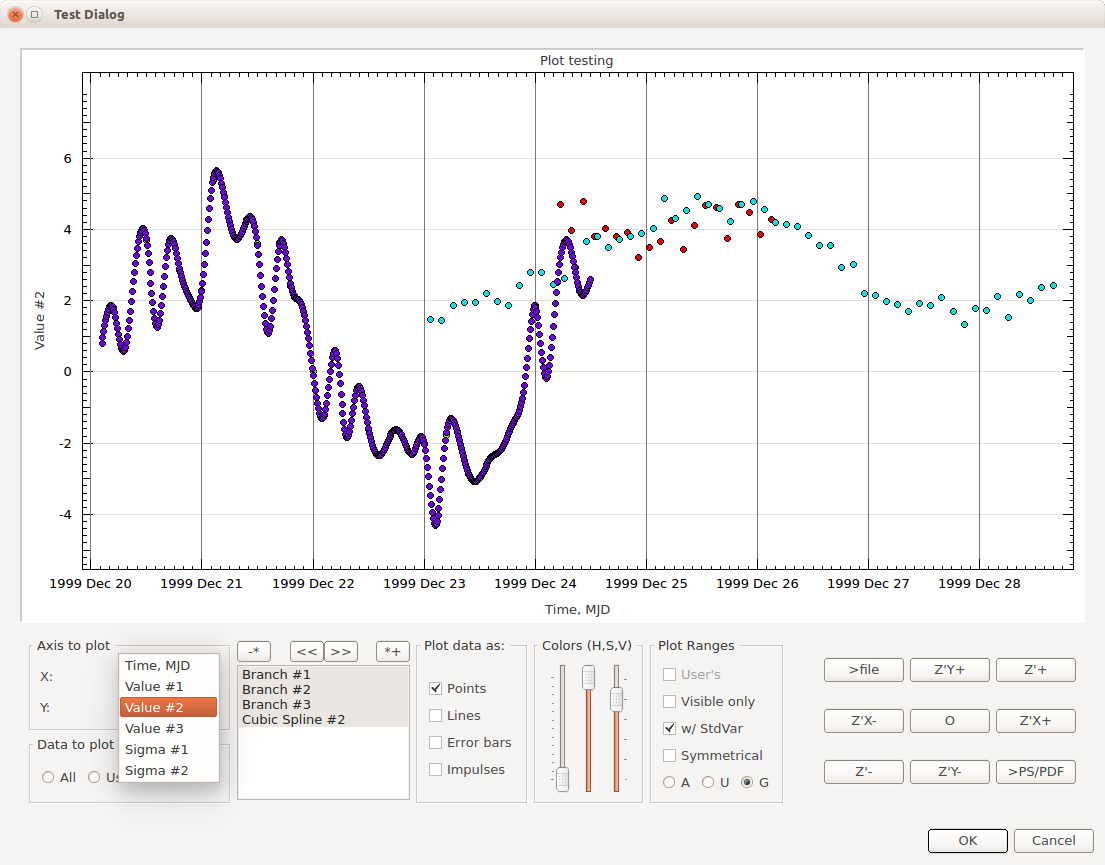
\includegraphics[width=0.45\textwidth]{plotter-controls-atp-1.jpg} \hspace{5mm}
    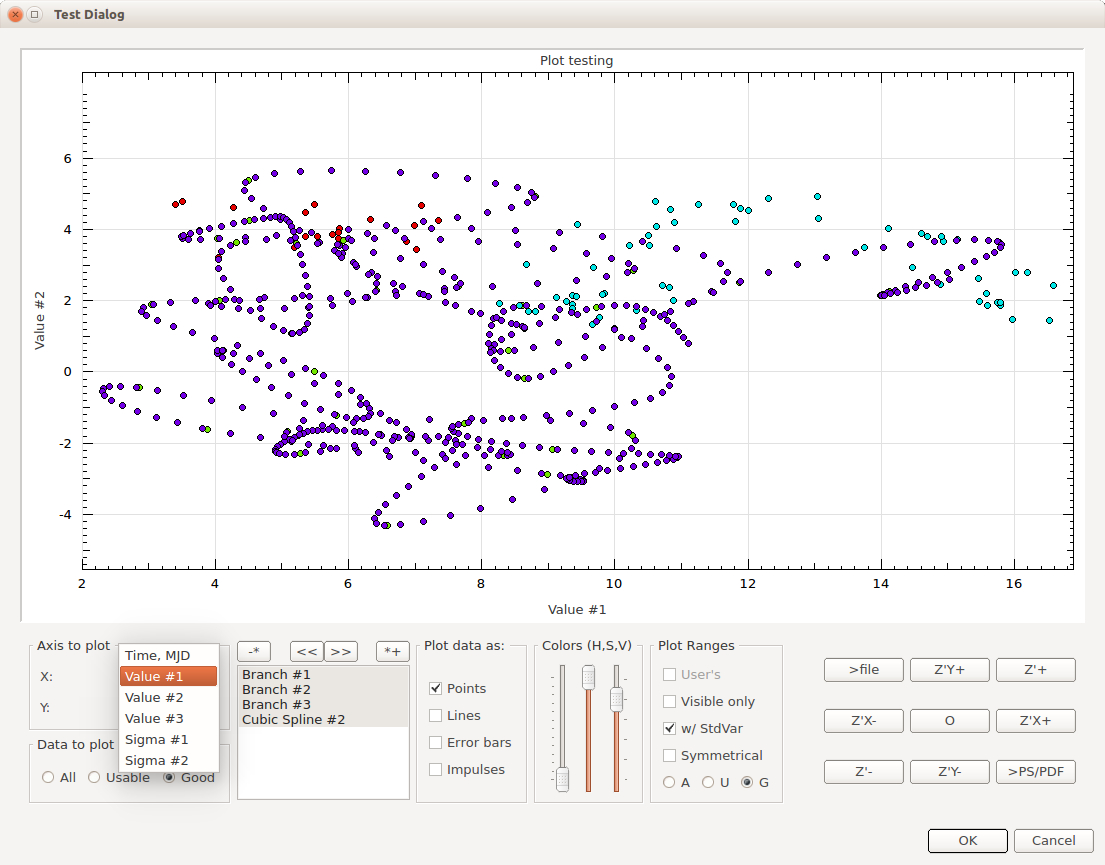
\includegraphics[width=0.45\textwidth]{plotter-controls-atp-2.jpg}
  \end{center}
  \caption{Selection of axis to plot.}
  \label{fig-plot-atp}
\end{figure}



\subsection{Branches}
The list of branches makes possible to select or deselect on the plot
some particular branch. The Fig.~\ref{fig-plot-bl} demonstrates a
selection of various branches on the plot. Also, there are two buttons:
{\sl -*} unselects all branches; and {\sl *+} selects all branches.
There are a couple of other buttons, {\sl \textless\textless} and {\sl
\textgreater\textgreater}, that allows a user to traverse through
branches going forward or backward one branch at a time.

\begin{figure}[htb!]
\begin{center}
    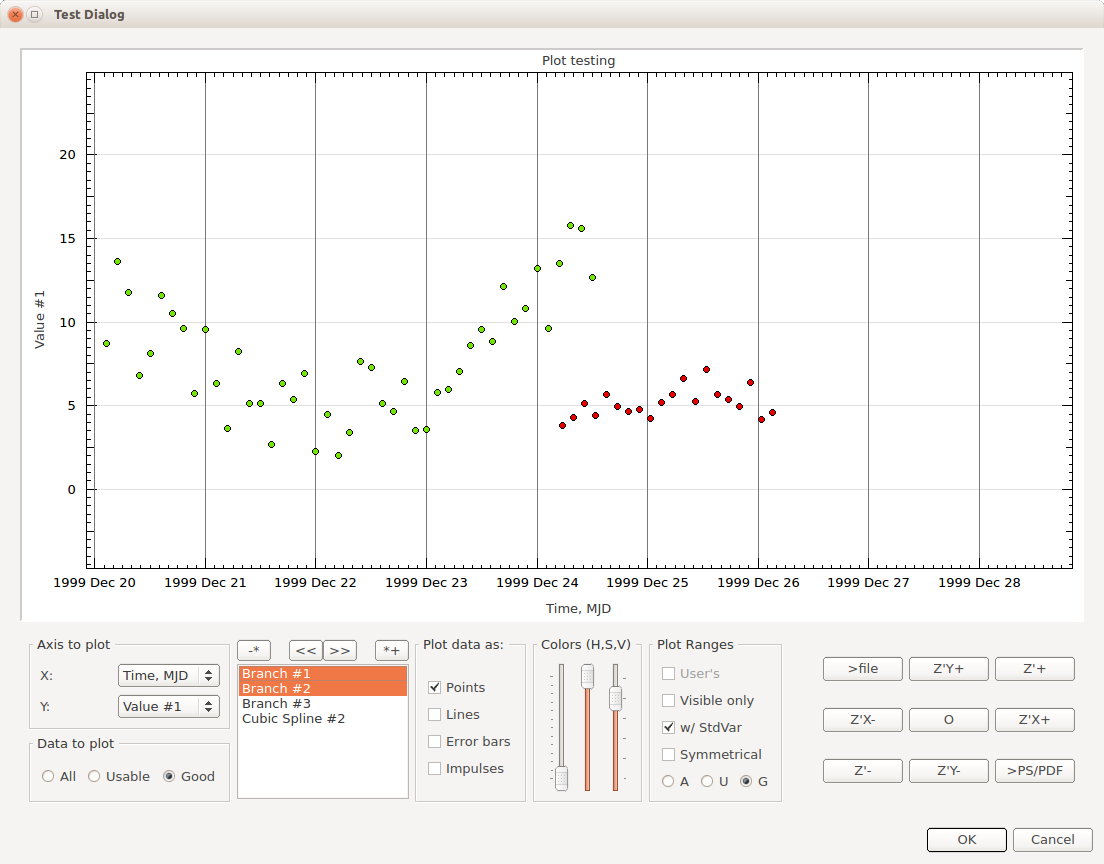
\includegraphics[width=0.45\textwidth]{plotter-controls-bl-1.jpg} \hspace{5mm}
    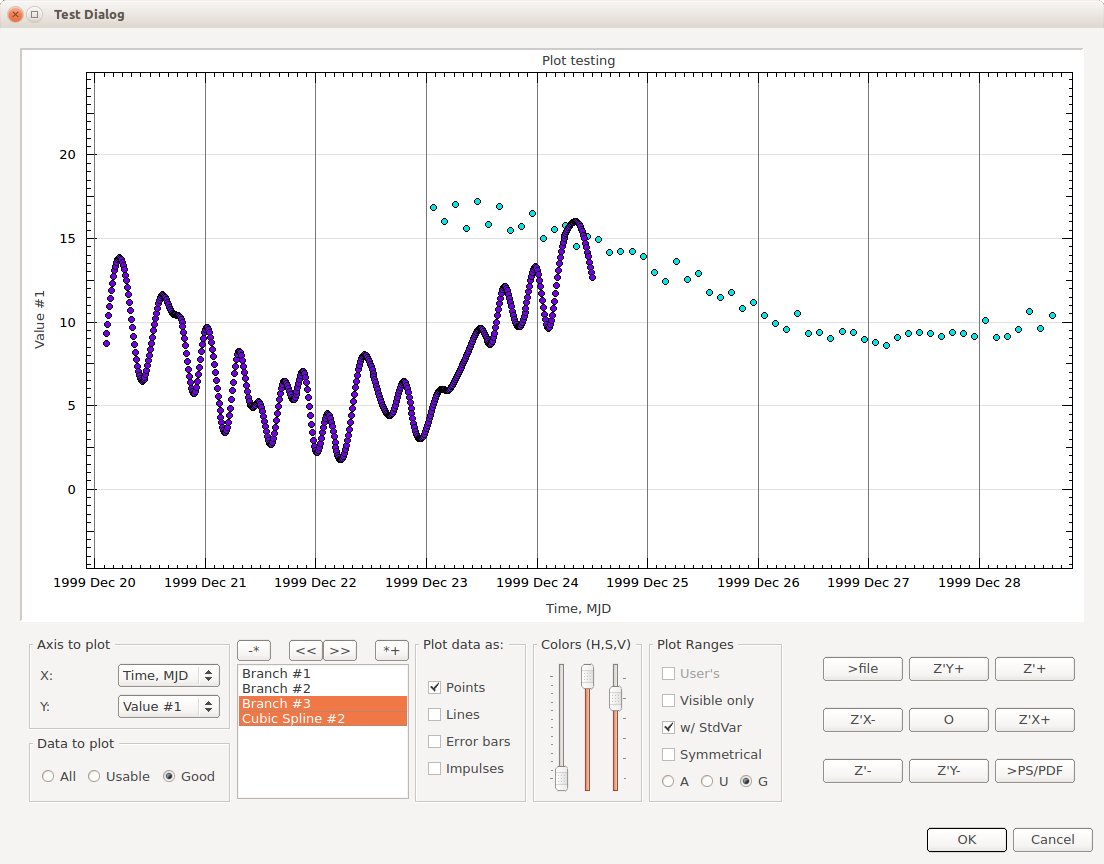
\includegraphics[width=0.45\textwidth]{plotter-controls-bl-2.jpg}
  \end{center}
  \caption{Selecting branches at the plot.}
  \label{fig-plot-bl}
\end{figure}



\subsection{How to plot data}
The group {\sl Plot data as} contains several checkboxes that specify
how to plot the data. Now it is possible to display data as points,
lines, errorbars and impulses. All modes are independent and can be
mutually combined.



\subsection{Altering colors}
Branch colors are assigned automatically, using HSV scheme. To modify
hue phase, saturation and value of the colors, use the slide bars from
the group {\sl Colors (H,S,V)}.



\subsection{Range controls}
The group {\sl Plot Ranges} controls how the plot ranges are
calculated. The check box {\sl User defined} becomes available if a
user specifies the plot ranges manually. To return back to automatic
plot range mode, uncheck this button. Current data model assumes that
there are two kind of points, <<good>> and <<discarded>>. By default,
only <<good>> points are plotted. To display all points on the plot,
check on the box {\sl All Data}. In this case all data will be
displayed and the plot ranges will be adjusted to make the <<discarded>>
data visible too. The check box {\sl Relaxed} turns on calculation of
the plot ranges only for selected branches. And the check box {\sl w/
StdVar} includes standard variations of the values in the calculation
of the plot ranges.



\subsection{Scale and output controls}
The last group of plotter controls contains a set of buttons that
perform the following functions. The rightmost top and leftmost bottom
buttons, {\sl Z'+} and {\sl Z'-} change the scale of whole plot in
one or another direction. The user can perform the same operations using
their mouse wheel (if their mouse has a wheel, of course.)

The rightmost and leftmost middle buttons, {\sl Z'X+} and {\sl Z'X-}
change the scale of X-axis on the plot. The keys {\sl Ctrl+RightArrow}
and {\sl Ctrl+LeftArrow} do the same.

The middle top and bottom buttons, {\sl Z'Y+} and {\sl Z'Y-} (as
well as keys {\sl Ctrl+UpArrow} and {\sl Ctrl+DownArrow}) change the
scale of Y-axis on the plot.

The central button, {\sl O}, restores the altered scales.

Pressing the button {\sl >file}, a user can save data (only selected
branches) as ASCII files for further processing. The format of the files
is simple, three columns, X, Y and standard variations of the Y column.
The button {\sl >PS/PDF} makes an output of the plot in Postscript or
PDF format.




%%%%%%%%%%%%%%%%%%%%%%%%%%%%%%%%%%%%%%%%%%%%%%%%%%%%%%%%%%%%%%%%%%%%%%%%%%%%
%%
%%
%%
%%%%%%%%%%%%%%%%%%%%%%%%%%%%%%%%%%%%%%%%%%%%%%%%%%%%%%%%%%%%%%%%%%%%%%%%%%%%
\section{Canvas}
The canvas also provides user controls. The communication between user
and canvas is performed by processing signals from a pointer device (a
mouse).

\begin{wrapfigure}{r}{0.22\textwidth}
\begin{center}
    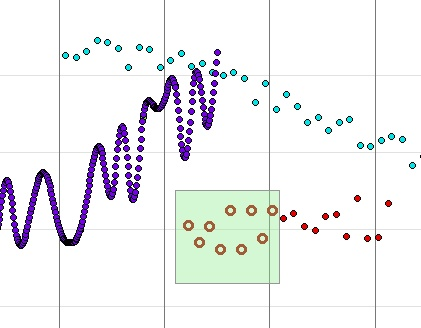
\includegraphics[width=0.21\textwidth]{plotter-controls-canvas-selection.jpg}
  \end{center}
  \caption{Selection of points on the plot.}
  \label{fig-plot-canvas-seletion}
\end{wrapfigure}

%\subsection{Selection}

Clicking the left mouse button when the cursor is on a point selects
this point. The selected points are displayed as open circles. A click
on a selected point discards the selection.

Clicking the right button of the mouse pointing anywhere on the canvas
displays the plot coordinates of the pointer location.

To select a group of points, hold the left mouse button down and drag
the mouse over the points, generating a rectangular area containing the
selected points (see Fig.~\ref{fig-plot-canvas-seletion}). All points
that appear inside this area will be marked as selected points. To
remove selection marks from a group of points, first, press the {\sl
Shift} key and then hold down the  left mouse button and drag the mouse
to create the area where all marked points will be deselected. In both
cases, the status of already altered points does not change. For
instance, if you make a selection, all previously selected points will
not became unselected and vice verse.

%\subsection{Measuring distances}

\begin{wrapfigure}{r}{0.22\textwidth}
\begin{center}
    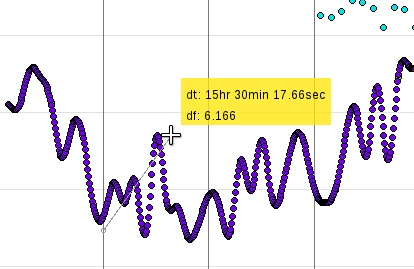
\includegraphics[width=0.207\textwidth]{plotter-controls-canvas-measurement.jpg}
  \end{center}
  \caption{Selection of points on the plot.}
  \label{fig-plot-canvas-measurement}
\end{wrapfigure}

By pressing and holding the {\sl Shift} key, clicking the right mouse
button, and dragging the mouse, you can measure a distance on the plot
between two points. The {\sl Shift} modifier is necessary only when you
press right mouse button, you can release the {\sl Shift} key, it does
not affect the measurement mode. Fig.~\ref{fig-plot-canvas-measurement}
shows how a user can acquire the distance between two points on the
plot.


%\subsection{Changing ranges}

Using the {\sl Ctrl} key and holding the right mouse button allows the
user to select a plotting range by dragging the mouse over a selected
area, thereby switching to manual range mode. When the user releases the
right mouse button, the ranges will be taken from the selected area and
applied to the plot. In contrast to the previous mode, the {\sl Ctrl}
key must be pressed when the mouse button is released, otherwise the
operation will be discarded. The Fig.~\ref{fig-plot-canvas-reranging}
displays the operation of changing the ranges. In the left panel, a user
selects the new ranges by dragging the mouse. The right panel shows the
plot with new ranges.

\begin{figure}[htb!]
  \begin{center}
%    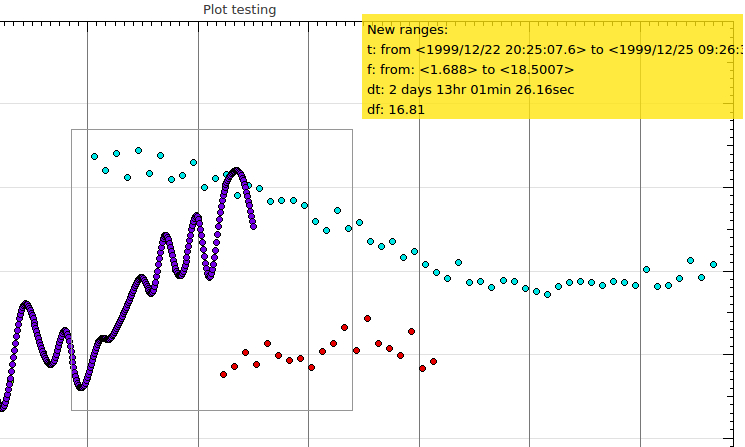
\includegraphics[width=0.53\textwidth]{plotter-controls-canvas-reranging-1.jpg} \hspace{5mm}
%    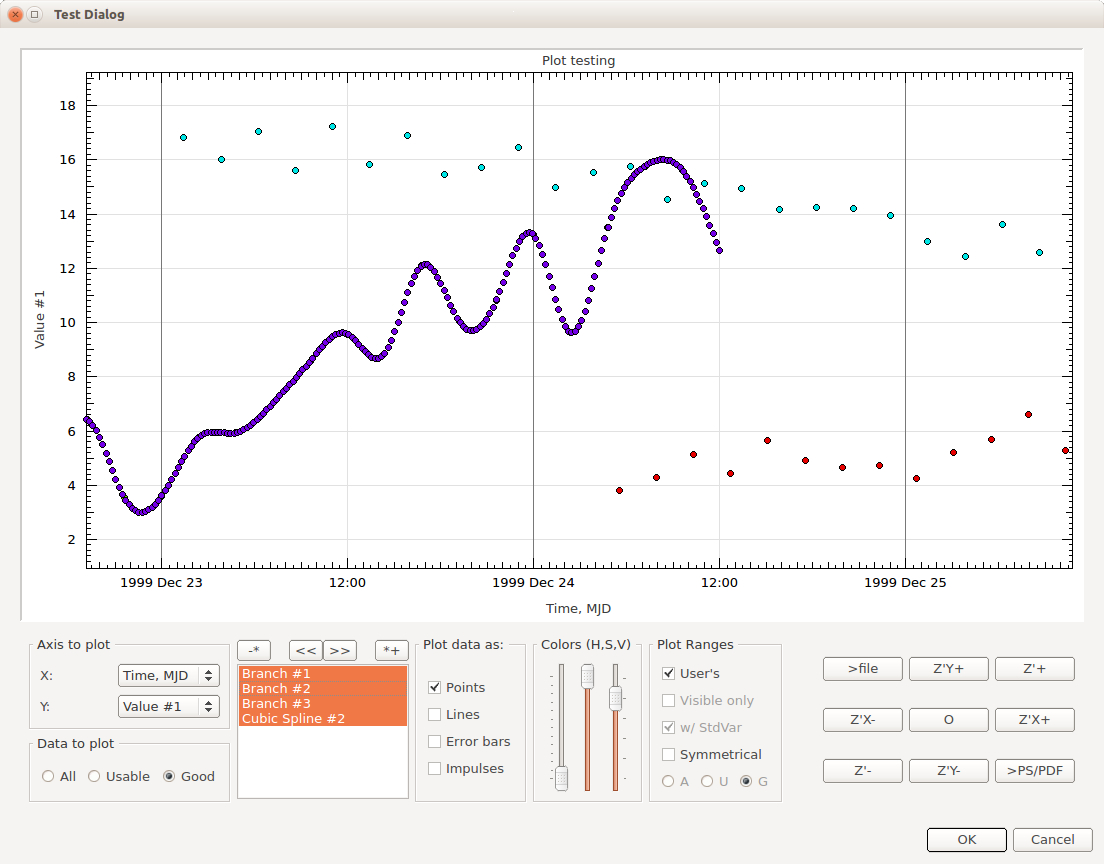
\includegraphics[width=0.37\textwidth]{plotter-controls-canvas-reranging-2.jpg}
    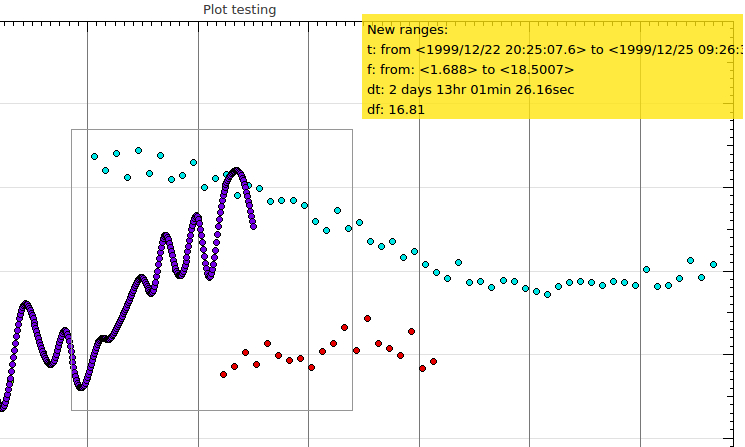
\includegraphics[height=0.25\textheight]{plotter-controls-canvas-reranging-1.jpg} \hspace{5mm}
    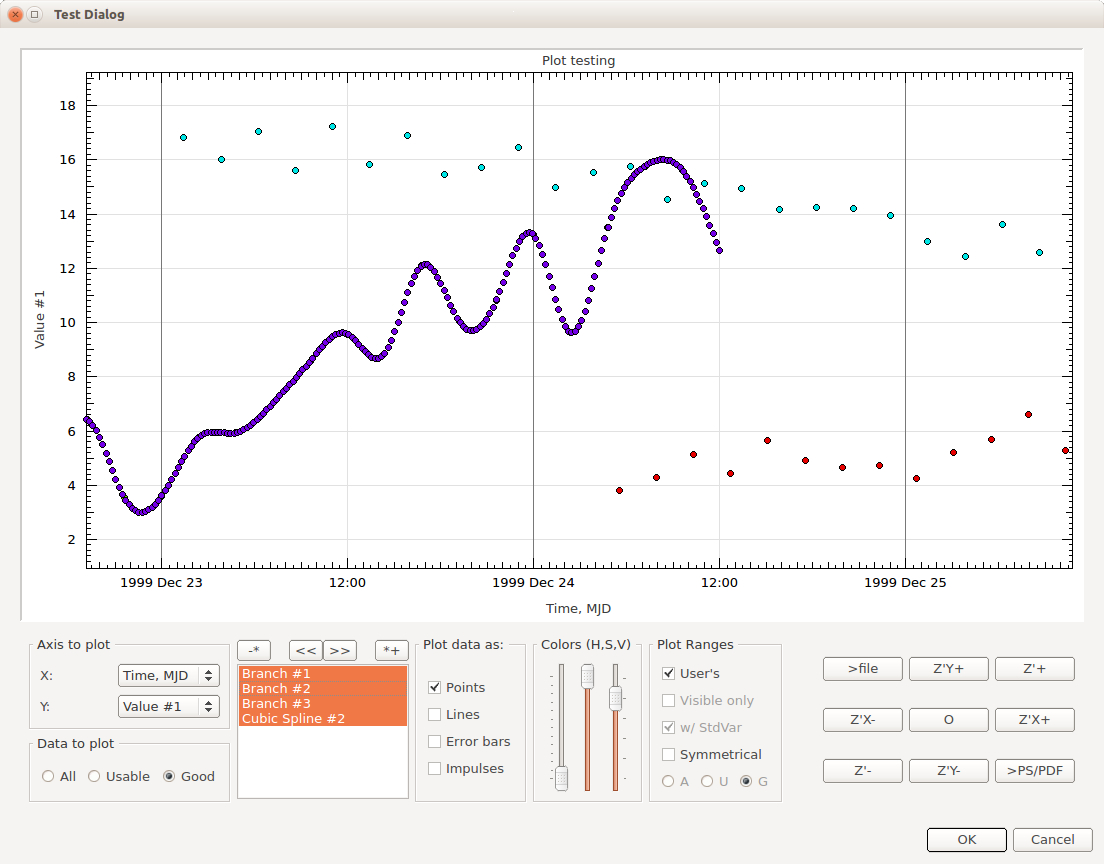
\includegraphics[height=0.25\textheight]{plotter-controls-canvas-reranging-2.jpg}
  \end{center}
  \caption{Changing ranges of the plot. Selecting new ranges (on left) and resulted plot with
  the new ranges (on right).}
  \label{fig-plot-canvas-reranging}
\end{figure}

When the plotter switches to the manual range mode, the checkbox {\sl
User defined} in the group {\sl Plot Ranges} on the plot window page
becomes available for user interaction and its status becomes <<on>>. To
return back to the automatic range mode (where the software will
evaluate ranges from the available data), just uncheck the checkbox.







%%%%%%%%%%%%%%%%%%%%%%%%%%%%%%%%%%%%%%%%%%%%%%%%%%%%%%%%%%%%%%%%%%%%%%%%%%%%%%
%
%
\chapter{Overview of the Session Editor window}

The Session Editor window is a primary tool for processing a VLBI session.
In this section we will review the essential parts of the window and describe
its interface with a user.

%
%

%%%%%%%%%%%%%%%%%%%%%%%%%%%%%%%%%%%%%%%%%%%%%%%%%%%%%%%%%%%%%%%%%%%%%%%%%%%%
%%
%%
%%
%%%%%%%%%%%%%%%%%%%%%%%%%%%%%%%%%%%%%%%%%%%%%%%%%%%%%%%%%%%%%%%%%%%%%%%%%%%%
\section{Reading a session}
\label{section-reading-session}

To invoke the Session Editor, the user must open an existing VLBI
session.

%\begin{wrapfigure}{r}{0.4\textwidth}
\begin{figure}[htb!]
  \begin{center}
    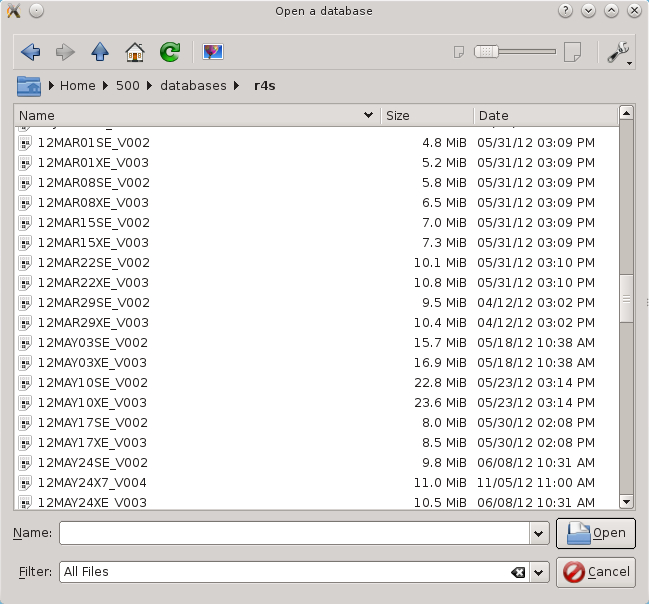
\includegraphics[width=0.6\textwidth]{open-dbh-s.jpg}
  \end{center}
  \caption{Opening a VLBI session in the standalone mode.}
  \label{fig-open-dbh-dog}
\end{figure}

The software can import a VLBI session in three formats, DBH, vgosDb
and vgosDa (formerly known as AGV format, see http://astrogeo.org/gvh/vda.html).


%Since the vgosDb format is still in the experimental phase, we discuss
%only DBH format here.

To read a session in DBH format, press {\sl Ctrl+e} or select menu
{\sl Edit-->Edit Session (DBH)}. Depending on
the software operation mode, standalone or working through catalog, a
dialog window will pop up.

In the standalone mode the dialog window is a Qt's standard file
selection dialog window, Fig.~\ref{fig-open-dbh-dog}.

The directory where it starts is taken from the preferences, {\sl
Observations (DBH) files}, however, a user can search through whole
file system to pick up a file. The user selects a file for the session
to be opened. Since a multiband VLBI session is represented by at least
two databases, generally, one for X-band and another one for S-band, the
software will automatically pick up a corresponding file with another
band (if it exists). If several files of the appropriate band exist, the
software will pick the file with the closest (but not larger) version
number of the file specified by a user.

In the catalog aware mode, the user enters the database name in a simple
window (see Fig.~\ref{fig-open-dbh-cat}).

\begin{figure}[htb!]
  \begin{center}
    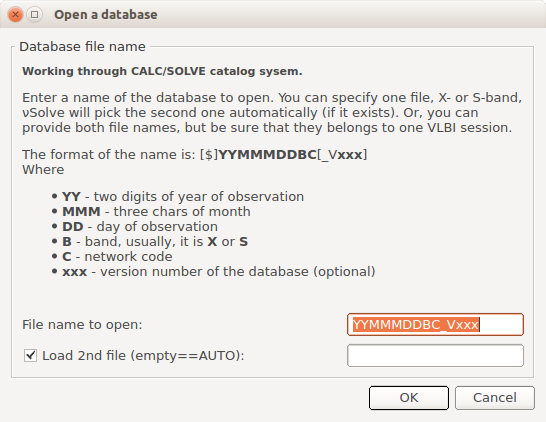
\includegraphics[width=0.5\textwidth]{open-dbh-c.jpg}
  \end{center}
  \caption{Opening a VLBI session in the CALC/SOLVE catalog aware mode.}
  \label{fig-open-dbh-cat}
\end{figure}

A database name is expected to follow the standard IVS naming
convention. Optionally, a version (in the standard form) can be
specified. If a file for a different band exists in the catalog, it will
be loaded automatically. To prevent automatic loading of the second band
database, set the checkbox {\sl Load 2nd file} to <<off>>. If a second
band database has an alternate name, you can specify it in the field
of {\sl Load 2nd file}. If the field is empty, the name of the second
band database will be figured out by the software using the IVS naming
convention.

The software will check database for the available versions and if the
next version is already registered in the catalog, it will issue a
warning about the inability to save the database as a new version. In
this case, the user can save his work, but before saving it, he should
remove the database with new version from the catalog manually before
saving the data.

There are two options to read a session in vgosDb format. The first one
allows a user to chose a wrapper file manually. The main menu option
{\sl Edit->Open Wrapper file (vgosDB)} or key combination {\sl Ctrl+o}
invokes a standard file dialog to select a desired wrapper file.

The second option chooses the latest wrapper file from a database name.
Press {\sl Ctrl+Shift+o} keys or select {\sl Edit->Open Session (vgosDB)}
from the main menu, a simple dialog window will appear and a user can
provide a name of a database. If the desired session exists in the standard
place, \nuSolve{} will read it.

To read a file in vgosDa format, press {\sl Ctrl+Shift+a} keys or
select {\sl Edit->Open VDA file}.




%
%
%%%%%%%%%%%%%%%%%%%%%%%%%%%%%%%%%%%%%%%%%%%%%%%%%%%%%%%%%%%%%%%%%%%%%%%%%%%%
%%
%%
%%
%%%%%%%%%%%%%%%%%%%%%%%%%%%%%%%%%%%%%%%%%%%%%%%%%%%%%%%%%%%%%%%%%%%%%%%%%%%%
\section{Session Editor}
\label{sect-session-editor}
After reading a database for a VLBI session, a Session Editor window
will appear, as in Fig.~\ref{fig-sessedit-gi}. This is a central window
for processing a VLBI session. The user can open as many windows as
his/her computer virtual memory allows. The user can open the same
session in several windows since the windows do not share the same data.
However, in the catalog aware mode saving the data will be possible only
if the corresponding version is available in the catalog. In the
standalone mode, if a database with new version already exists, the file
name of the saved data will be altered.

\begin{figure}[htb!]
  \begin{center}
    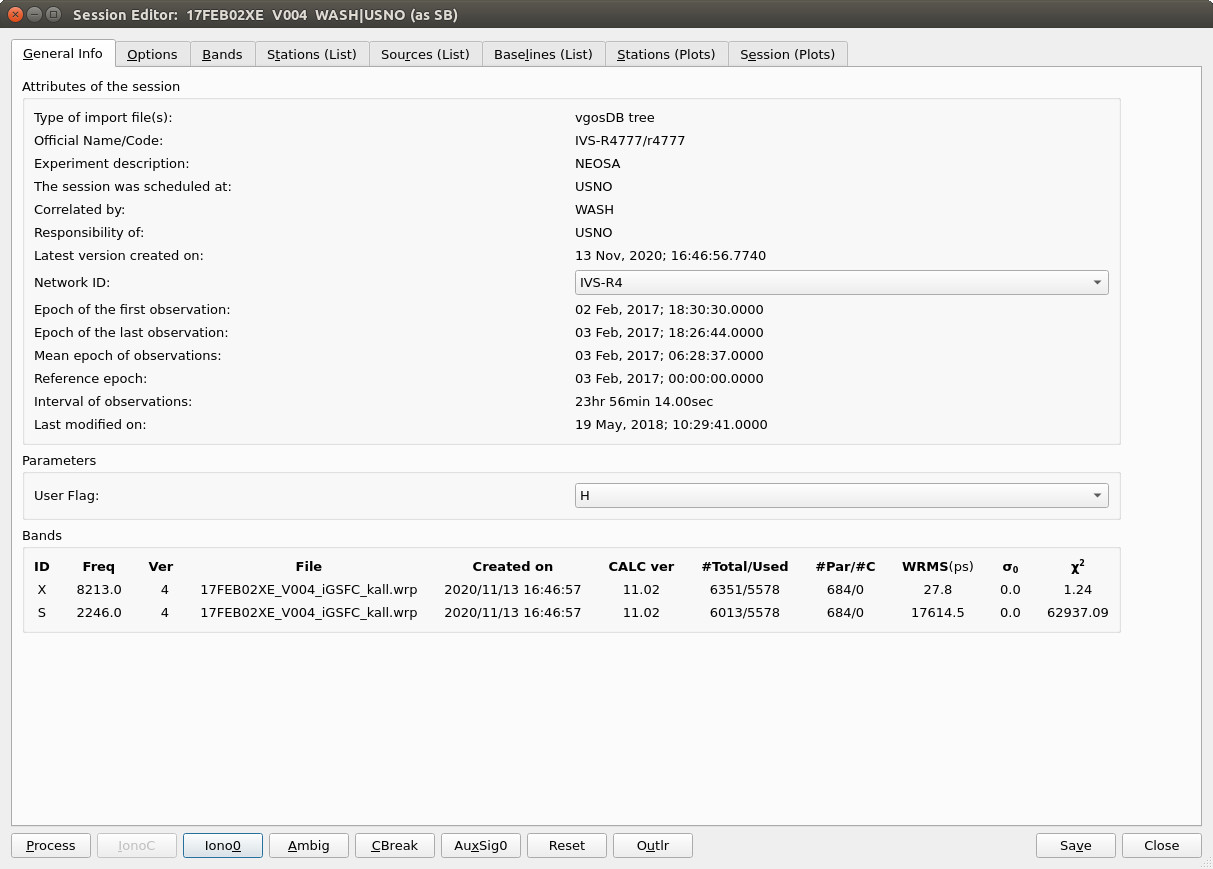
\includegraphics[width=1.0\textwidth]{sessedit-gi.jpg}
  \end{center}
  \caption{Session Editor window, general info.}
  \label{fig-sessedit-gi}
\end{figure}

The Session Editor window consists of several tabs along the top of the
window and a row of buttons along the bottom. The {\sl General Info}
tab provides general information about the session. From the {\sl
Options} tab the user can find controls to choose options for how to
process a session. The {\sl Bands} tab refers to separate bands in
order to display of selected data as plots, allow control of
band-specific parameters, etc. The tabs {\sl Stations (List)}, {\sl
Sources (List)} and {\sl Baselines (List)} make it possible to
manipulate data using the stations, sources or baselines attributes. The
{\sl Stations (Plots)} tab displays station-dependent data. The last
tab, {\sl Session (Plots)}, is designed to test Earth rotation parameters
that are estimated as arc, PWL or stochastic parameters. It is
currently in a test mode and will be discussed in the next release
of the software.

Pressing one of the buttons causes \nuSolve{} to perform some particular
action. The button {\sl Process} performs one iteration of parameter
estimation. {\sl IonoC} evaluates ionospheric corrections and {\sl
Iono0} discards these corrections (sets them to zero). The button {\sl
CBreak} initiates a procedure of clock break detection. To perform an
outlier processing action the user should press the {\sl Outlr}
button. To resolve ambiguities,the user would press the {\sl Ambig}
button. The button {\sl AuxSig0} sets to zero any previously evaluated
weight correction sigmas.

The user saves an updated session in a file on the hard drive by
pressing the button {\sl Save}. The button {\sl Close} will close
the Session Editor window. If the preferences check box {\sl Warn me
when closing Session Editor Window} is <<off>>, the window will close
without any warnings and if there were unsaved data (the autosave mode
in Preferences was set to {\sl None}), it will be lost.

The button {\sl Reset} clears all editing information. A VLBI session
will look like newly arrived from a correlator.

In addition to buttons, there are shortcuts (combinations of keys) that
invoke actions. For example, if the user presses the {\sl Ctrl+r} keys,
\nuSolve{} will generate a report in a CALC/SOLVE spoolfile format (by
default, such a report is generated when a user saves a processed VLBI
session). The list of available key combinations is in Table~\ref{tab-shortkeys}.
Some of the shortcuts will be discussed later.

\begin{table}[h]
\centering
\begin{tabular}{l p{0.75\textwidth}}
\hline
Shortcut          & Action \\
\hline
{\sl Ctrl+a}      & Exports estimated source positions and station coordinates
                    (aposteriori info) with applied velocities in a format of
                    the a priori files.\\
{\sl Ctrl+b}      & Process a clock break for the marked observation.\\
{\sl Ctrl+f}      & Generate a list of commands to refringe marked observations.\\
{\sl Ctrl+g}      & Store a VLBI session in vgosDa format.\\
{\sl Ctrl+h}      & Creates ASCII files with results of estimation the stochastic
                    parameters.\\
{\sl Ctrl+i}      & Displays a window with lists of unusable and excluded
                    observations.\\
{\sl Ctrl+n}      & Exports a VLBI session in NGS format.\\
{\sl Ctrl+r}      & Generates a report in a CALC/SOLVE spoolfile format.\\
{\sl Ctrl+Shift+r}& Generates a report in a CALC/SOLVE spoolfile format.
                    In addition, prints the residuals and other information
                    to the spoolfile.\\
{\sl Ctrl+s}      & Saves the intermediate results in a file.\\
{\sl Ctrl+t}      & Performs a test of an action, for test purposes only.\\
{\sl Ctrl+z}      & Creates ASCII files with values of total zenith delays.\\
{\sl Alt+2}       & Makes two consecutive iterations of parameter estimation.
                    The same as two clicks on {\sl Process} button.\\
{\sl Alt+3}       & Makes three consecutive iterations of parameter estimation.\\
{\sl Alt+4}       & Performs outlier processing and then calls three iterations
                    of parameter estimation. Equivalent to click on {\sl Outlr}
                    button and then {\sl Alt+3} shortcuts.\\
\hline
\end{tabular}
\caption{Shortcuts of Session Editor window.}
\label{tab-shortkeys}
\end{table}


%
\subsection{Tab <<General Info>>}
From the {\sl General Info} tab, the user can find various attributes
of the session. In most cases, the names of attributes are self
explanatory, see Fig.~\ref{fig-sessedit-gi}. A user should ignore
{\sl User Flag} (in {\sl Parameters} group) since this refers to future
features that have not been implemented.

The group {\sl Bands} displays available bands, their parameters, the
number of all and processed or <<good>> observations (the column {\sl
\#Total/Used}), the number of estimated parameters and applied
constraints (the column {\sl \#Par/\#C}), and the overall weighted
root-mean- squared (the column {\sl WRMS(ps)}) of the delay residuals
for each band. The last two columns of the group show the sigma for
weight correction (the column {\sl $\sigma_0$}), where this value is non
zero if weight corrections have been performed in the band-wide mode,
and a value of the reduced $\chi^2$ of the residuals for each of the bands.



%
\subsection{Tab <<Options>>}
\label{subsect-sessedit-options}
The tab {\sl Options} was discussed in details in Section~\ref{sect-config}.
There are few exceptions: some widgets have different layout and the
tab {\sl Post import actions} of {\sl Options} is not shown.

%
\subsection{Tab <<Bands>>}
\label{subsect-sessedit-bands}
The tab {\sl Bands} consists of several embedded tabs
(Fig.~\ref{fig-sessedit-bands}), that allow the user to display a
relatively large amount of data on one screen. The main purpose of this
tab is represent observations and baseline dependent values as plots. It
also allows the user to edit data.

Starting with version 0.7.0 of the distribution the tab has an ability to filter
data on per source basis (if the corresponding option of Preferences is selected).
On the right of the tab there is a listview widget that contains names of sources.
A user can select or deselect sources, the plot displays data only for sources
that are highlighted in the listview widget.


\begin{figure}[htb!]
  \begin{center}
    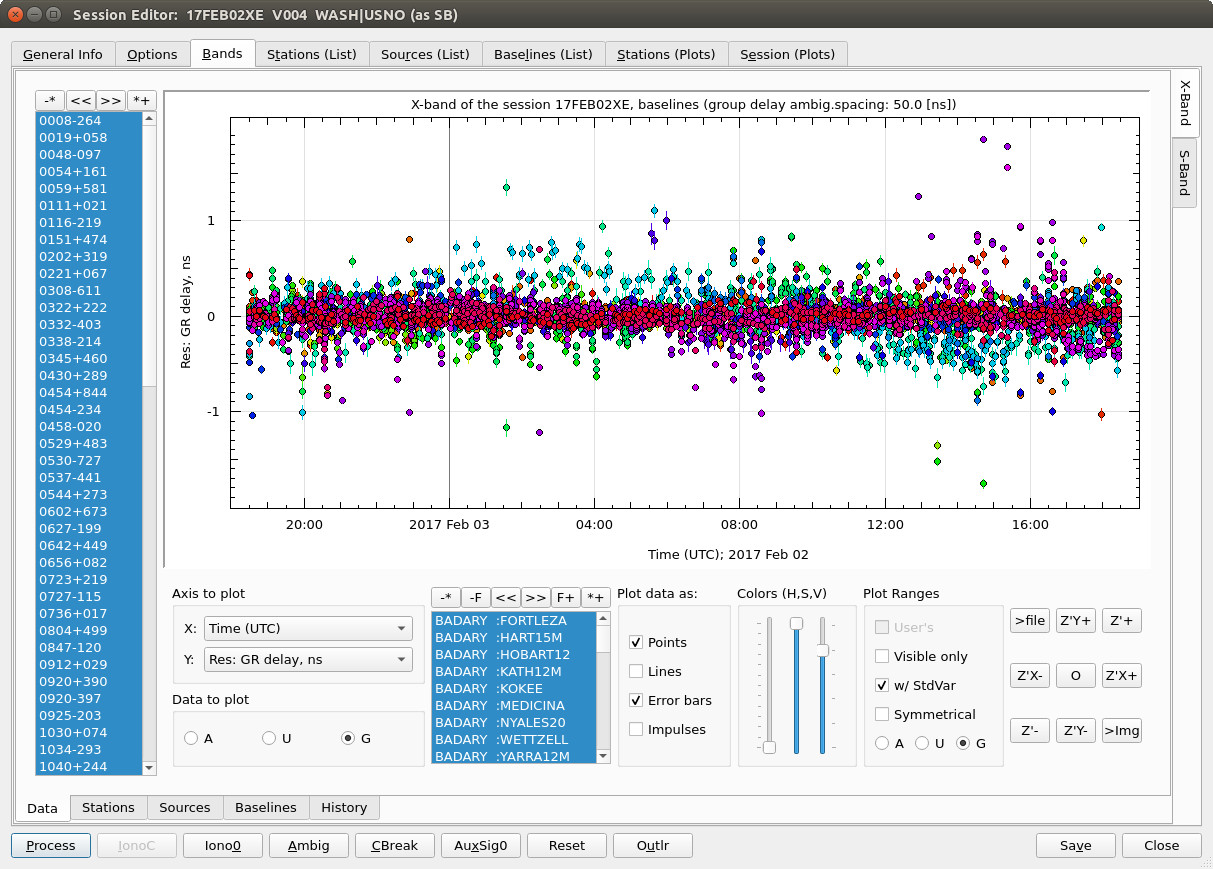
\includegraphics[width=1.0\textwidth]{sessedit-bands.jpg}
  \end{center}
  \caption{Session Editor window, band dependent plots and attributes.}
  \label{fig-sessedit-bands}
\end{figure}

At the bottom of the plot there are tabs that display information about
the particular band. The tab {\sl Data} shows plots. The tabs {\sl
Stations}, {\sl Sources} and {\sl Baselines} displays statistics (number
of total observations, number of used observations, dispersions,
additional sigmas and residuals for delay and rate) per station, source
and baseline respectively. In addition, in the tab {\sl Stations}, the
user can add or modify band-dependent clock breaks for some particular
station. Also, the tab {\sl Baselines} displays ambiguity spacings and
typical numbers of channels.

The interface of the last three tabs are the same as for corresponding
objects of the whole VLBI session. They will be discussed later.

\begin{figure}[htb!]
  \begin{center}
    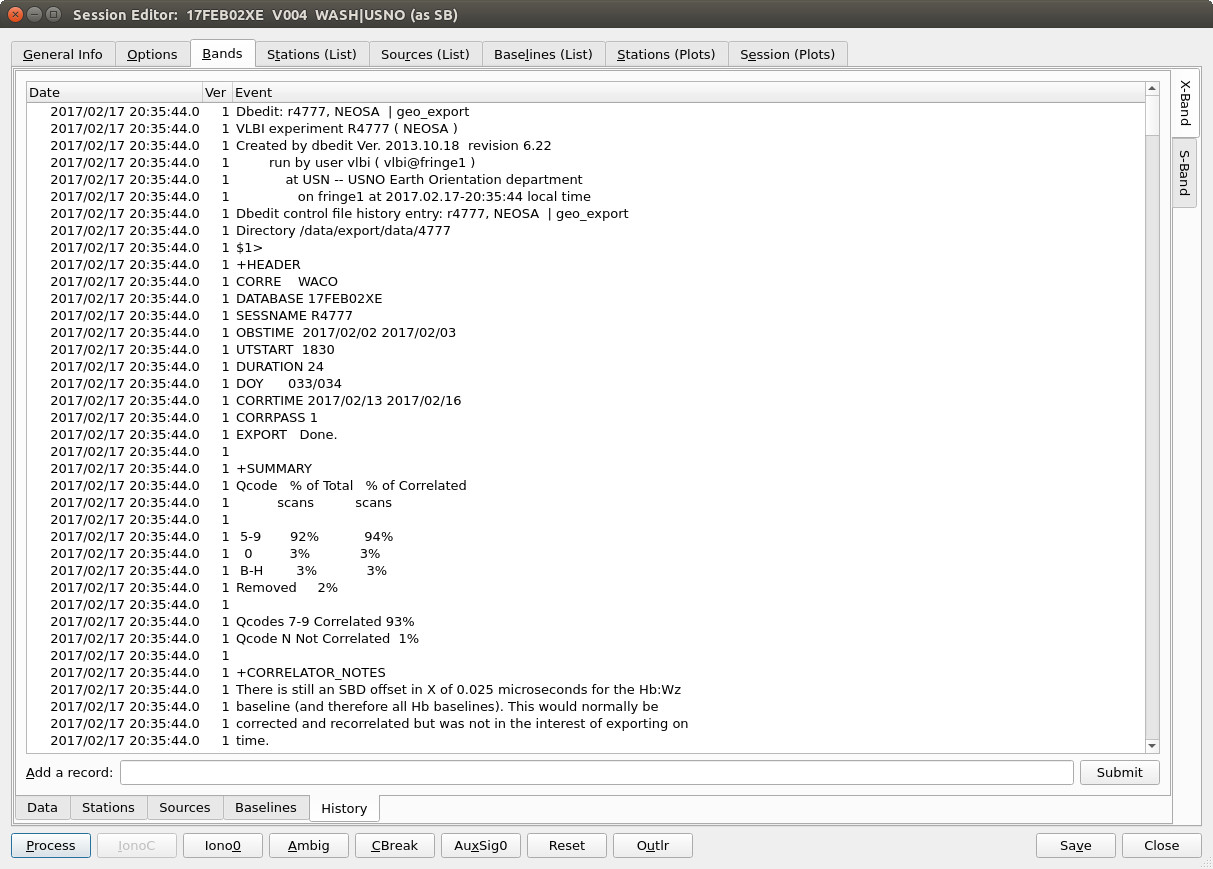
\includegraphics[width=1.0\textwidth]{sessedit-bands-hist.jpg}
  \end{center}
  \caption{Session Editor window, history records for the band.}
  \label{fig-sessedit-bands-hist}
\end{figure}


The tab {\sl History}, Fig.~\ref{fig-sessedit-bands-hist}, presents
the history records from the history part of a database file. It also
allows the user to add comments about processing a session (history
records) manually.

Plots in the {\sl Data} tab display baseline dependent values, such as
residuals, ionospheric corrections, etc. Each baseline on the plot is
represented by a branch of the plotter system. In the list of branches
there are two additional buttons, {\sl --F} and {\sl F+}. The buttons
activate filters that will be applied to the list of baselines to
select, {\sl F+}, or deselect, {\sl --F}, some particular baselines.

A left mouse click on the button invokes a local menu with a list of
stations. By selecting one of the stations, the user can select or
deselect all baselines with this station.

The right mouse click invokes
a menu with stations as the first or second station in the baseline. For
example, if the user makes a right mouse click on the button {\sl F+}
and selects {\sl KOKEE:} from the menu, then all baselines where the
KOKEE station is the reference site will be selected.

A left mouse click on the button {\sl F+} when a {\sl Shift} key is
pressed invokes a menu with a list of sources. If a user selects a source
from this menu, all observations (currently visible or not) will be
highlighted as open circles (selected). The same click on the button {\sl --F}
will deselect previously selected observations with the source from the menu.

%\begin{figure}[htb!]
%  \begin{center}
%    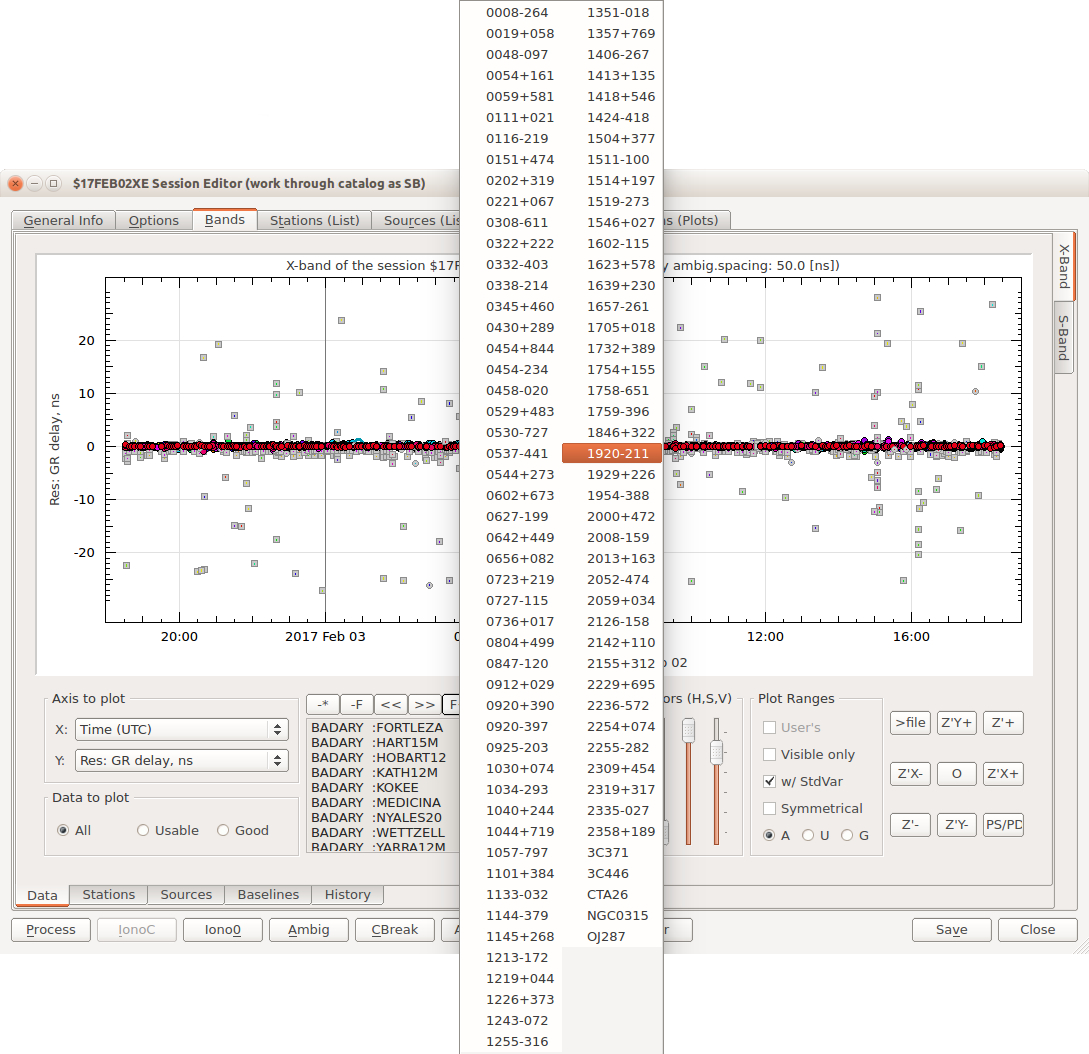
\includegraphics[width=1.0\textwidth]{sessedit-bands-src-selecting.jpg}
%  \end{center}
%  \caption{Session Editor window, highlighting the source .}
%  \label{fig-sessedit-bands-src-selecting}
%\end{figure}


The radio buttons at the bottom of the widget group {\sl Plot Ranges}
control ranges of plots to display data: used in the latest solution
({\sl G} -- good observations), potentially usable but deselected by
a user or outlier elimination procedure ({\sl U} -- usable observations)
and all available ({\sl A}) observations. What subset of data to
display on plots is switched by radio buttons in the widget group
{\sl Data to plot}.

The plotters of the {\sl Data} tabs have their own sets of shortcuts.
When the user selects one or several points, pressing the {\sl Ctrl+x}
key combination removes the marked point(s). Removing points means that
these observations will not be used in data analysis. In this case a
flag <<do not use>> is raised for the points. To discard the flag, user
should turn on the checkbox {\sl All Data} of the group {\sl Plot
Ranges} of plotter; then all unselected points will appear gray. Then,
select the points and press the {\sl Ctrl+y} key combination. The
latest operation does not force an observation into analysis, there can
be other criteria that remove observations from analysis (e.g., low
quality factor).

Another operation that can be applied to selected points, are for
increasing (key {\sl ``=''}) or decreasing ({\sl ``--''}) the number of
ambiguities. In these cases the number of ambiguities are increased or
decreased by one and the residuals for the group band delays are
adjusted using values of the ambiguity spacing.

The key combination {\sl Ctrl+b} is used to process a clock
break in a semi-automatic mode (see the next section).

A double click on an observation point opens an observation information
window, Fig.~\ref{fig-sessedit-bands-obs-info}. The window is modal, i.e.,
it blocks access to other windows of the software. To continue, press
the button <<Ok>>.


\begin{figure}[htb!]
  \begin{center}
    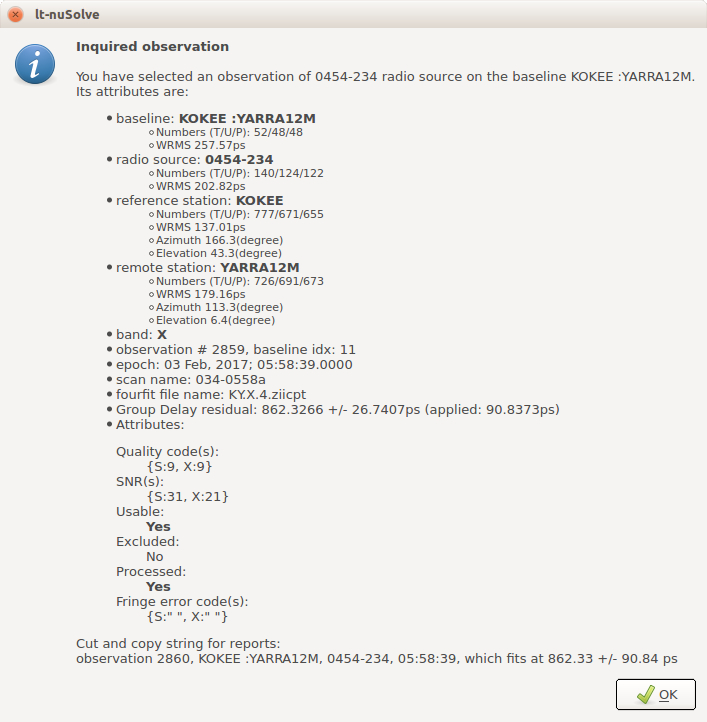
\includegraphics[width=0.5\textwidth]{sessedit-bands-obs-info.jpg}
  \end{center}
  \caption{Session Editor window, the observation info window.}
  \label{fig-sessedit-bands-obs-info}
\end{figure}

This window displays source and stations names, statistical information
(numbers of good, usable and processed observations and WRMS for delays)
for the baseline, the source and each of stations. Also, there are
information on delay residual value, its standard deviations, and the applied
standard deviations (which is usually bigger than the standard deviation of
the delay). If an observation considered as <<unusable>>, there will
be a reason of such decision: low quality code, deselected station, source or
baseline, missed observation on another band (if ionospheric corrections are
evaluated), and so on.


% Start of DGG ------------------------------------------


\subsection{Tab <<Stations (List)>>}
\label{subsect-sessedit-stations-list}
The tab {\sl Stations (List)} shows properties of the stations. It
organizes them as a table, as in Fig~\ref{fig-sessedit-stations-l}. A
mouse click on the header of the table sorts the whole table by fields
in this column.

\begin{figure}[htb!]
  \begin{center}
    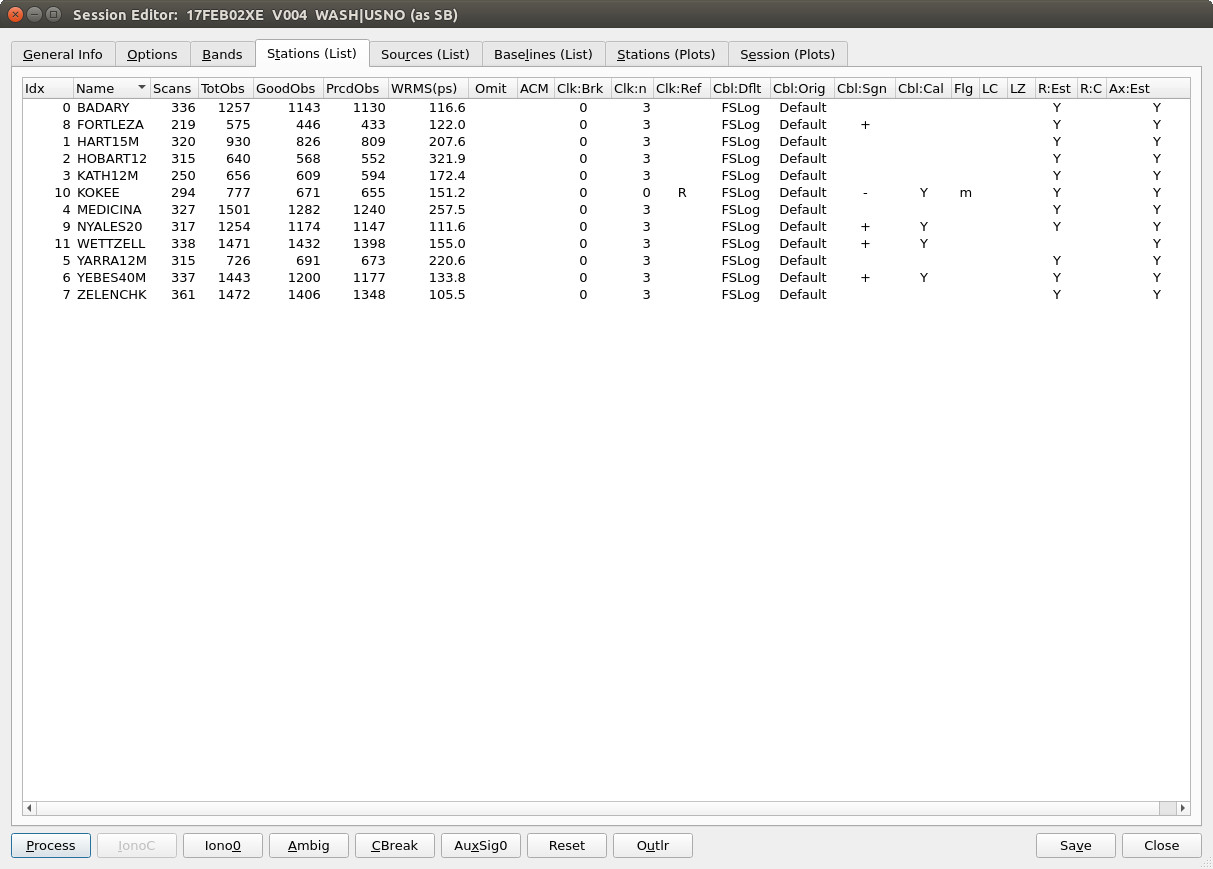
\includegraphics[width=1.0\textwidth]{sessedit-stations-l.jpg}
  \end{center}
  \caption{Session Editor window, list of stations.}
  \label{fig-sessedit-stations-l}
\end{figure}

The following station attributes are available: The number of scans, {\sl Scans}
the total, potentailly usable and processed
number of observations made by a station, {\sl TotObs}, {\sl GoodObs} and {\sl
PrcdObs}. Residuals of
group, single band or phase delays for a station are in {\sl WRMS(ps)}
column.

The column {\sl Omit} displays a flag if a station is deselected from
data analysis. The user can set this flag by clicking the mouse button
with the mouse pointer in this column. If the station is turned off, a
char {\sl X} will appear in this column. The user can click and drag
the mouse pointer to select/deselect a group of stations.

The column {\sl ACM} indicates the stations with a priori clock
model. Sometimes, station clocks could have a large offset, one or more
seconds. It is recommended to add a priori clock model for such case
otherwise global SOLVE will be unable to process a session. The column
{\sl Clk:Brk} represents numbers of clock breaks per each station.
The number of polynomials in the polynomial model for the clock function
are in the column {\sl Clk:n}. The left mouse button click
decreases the number and the right button increases it. The user can
click and drag the mouse pointer to decrease/increase the number of
polynomials for a group of stations.
The reference clock flags are displayed in the column {\sl Clk:Ref}.
A mouse button click toggles this flag. If you do not assign a reference
clock status to any stations, the standard deviations of clock
parameters will be on the level of their {\it a~priori} sigmas (i.e.,
very big). Also, you can set the number of polynomials of a reference
station to zero, in this case the clock model for that station will not
be estimated. If the {\sl Clk:n} is greater than zero and the
reference clock flag is set, then \nuSolve{} will apply constraints to
clock parameters of the station. Usually, for a regular VLBI session
there should be only one reference clock station. However, in rare cases
a network can contain two separate subnetworks. In such a case, you have
to assign two reference clocks, one from each separate subnetwork.

The column {\sl Cbl:Dflt} contains information about origin of default
cable calibration corrections for a station. There can be the following
values in the column: {\sl N/A}, {\sl FSLog}, {\sl CDMS} and
{\sl PCMT}. The default cable calibration corrections corresponds to the
standard cable corrections that are in the database and are using by all
data analysis software. In addition, the utility vgosDbProcLogs can collect
and store cable calibration data from other sources (if they are available).
For test purposes, nuSolve can use these types of data too (instead of
default). What type of cable calibration origin to use is spacified in
the column {\sl Cbl:Orig}. If more than one type of data is available,
a user can change the origin of cable calibration corrections using
the station attributes editor window (see below).
%\subsubsection{Station Attributes Editor}
%\label{subsubsect-sessedit-station-attr-editor}
The next column, {\sl Cbl:Sgn}, shows what sign has been applied to
cable calibration readings for each station (see vgosDbProcLogs User
Guide).

The column {\sl Cbl:Cal} shows whether the cable calibration data
from each each station are used or not. In general, we use cable
calibration data. However, if the correlator applied manual phase
calibration, then we normally do not use the cable calibration data.
Also, some stations provide cable calibration data that degrade the
solution. To turn off cable calibration data for some station, click
the mouse button in the column.

The {\sl Flg} column is designed to display various station flags. This
column currently shows the following station flags: "do not
estimate zenith delay" and "wrong meteo parameters".
For test purposes there is the ability to turn off
zenith delay estimation for some particular station (see below). In this case a
{\sl -Z} will be shown in the column. If a flag "wrong meteo parameters", {\sl m},
is set, \nuSolve{} uses standard atmospheric temperature, pressure and
relative humidity instead of what is present in a database.


It is possible to override parameters set up for clock and zenith delay
of a station. In general, a user configure estimated parameters in the
tab {\sl Options}. Sometimes, it is necessary to alter the
configuration of the parameter for some particular station. Most
frequent use of this feature -- large variations of clocks during one
session. In this case we loose the constraints that are applied to
the piecewise-continuous parameter of the estimated clocks of the station.
The columns {\sl LC} and {\sl LZ} show flags of use of local clocks
and local zenith. If for some station one of
the columns has the character {\sl Y}, a station specific configuration
of the estimated parameters will be applied for the station. A user can
adjust parameters of local clocks or local zenith delay with the station
attributes editor window (see below).

The column {\sl R:Est} displays which station positions will
be estimated if the user decided to estimate station positions on the
{\sl Options} tab. The character {\sl Y} means that the particular
station's coordinates will be estimated if the user set the radio button
of {\sl Station Coordinates} on the {\sl Options} tab to anything
except {\sl No}. This column only sets the status of this flag; it
does not turn <<on>> or <<off>> the estimation of station positions.
%In other words, this flag does not turn on or off estimation of station
%positions, but it will be taken into account if a user told the
%estimator to do so.

A mouse click in the {\sl R:C} column triggers the flag
for a station to participate in the equations of constrains. For
example, if the user wants to estimate EOP, source coordinates and
station positions, then he/she must apply the No-Net-Translation and
No-Net-Rotation constraints to the stations coordinates. All stations
that have a {\sl *} mark in this column will be involved in equations
of constrains. If no stations are marked, the equations of constrains
will not be applied.

And the column {\sl Ax:Est} controls for which station(s) the axis
offset will be estimated if a user decided to estimate axis offsets
(on the tab {\sl Options}). By default, for all stations this flag
is turned <<on>>.


\subsubsection{Station Attributes Editor}
\label{subsubsect-sessedit-station-attr-editor}
\begin{figure}[htb!]
  \begin{center}
    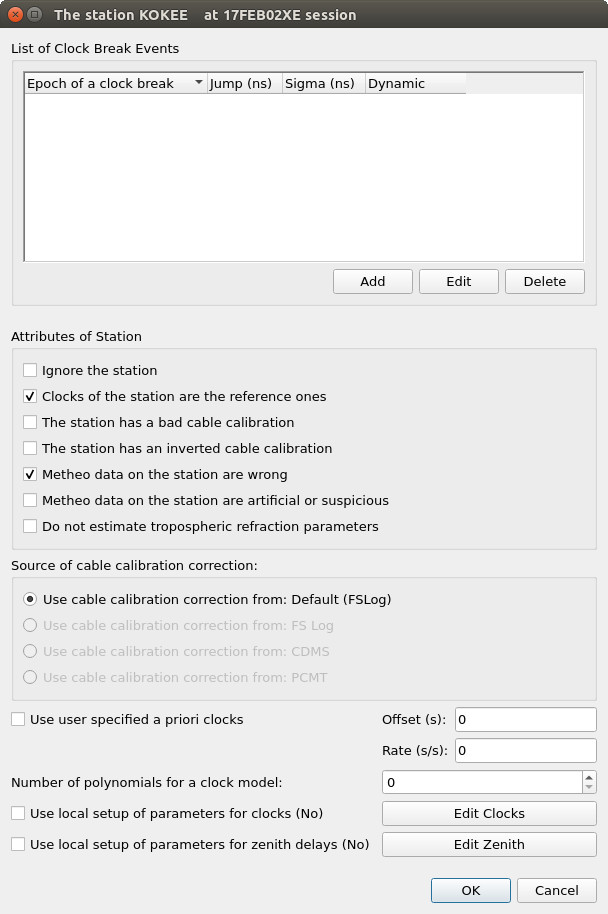
\includegraphics[width=0.35\textwidth]{stnedit-general.jpg}
  \end{center}
  \caption{Station attributes edit window.}
  \label{fig-stnedit-general}
\end{figure}
A double mouse click in the area bounded by columns {\sl Idx} and {\sl
Clk:Brk} invokes a station attributes editor window (see
Fig.~\ref{fig-stnedit-general}). This window allows a user to add,
modify or delete clock break events and turn <<on>> or <<off>> all
available stations attributes (some of them are accessible from the
station list, some are not).

The upper group of widgets allows the user to edit clock break data for
stations. The group consists of the list of clock breaks and three
buttons. In general, clock breaks occur infrequently and the list is
often empty. But if there is a break, \nuSolve{} can apply it in automatic,
semi-automatic and manual modes. The first two modes will be discussed
in the next chapter. In manual mode, the user must explicitly specify
the information about clock breaks. To do so, click the {\sl Add}
button and a clock break editor window will appear (it will be described
latter). To alter the parameters of a clock break, highlight the break
in the clock break list and press the {\sl Edit} button. The last
button, {\sl Delete}, removes a selected clock break from the list.

The lower group represents all available station attributes (some of
them can be altered by interacting with the stations list). Currently
there is just one station attribute that can be altered only with this
window, {\sl Do not estimate tropospheric refraction parameters}. If
the corresponding check box is <<on>>, then the tropospheric zenith
delay and its gradients for this particular station will be excluded
from the list of estimated parameters when the user tells the software
to estimate them.

The widget group {\sl Source of cable calibration correction} allows a user
to change a type of cable calibration correction (if data are available).
Using the value "Default" corresponds to data that are in the
Cal-Cable*.nc netCDF file.

To add {\it a priori} clock offset and rate, turn <<on>> the checkbox
{\sl Use user specified a priori clocks} and provide values of the
offset and the rate in the corresponding fields. This option is
implemented for consistency with global SOLVE.

The check boxes {\sl Use local setup of parameters for clocks} and
{\sl Use local setup of parameters for zenith delays} indicate that
\nuSolve{} should apply a unique parameter set up for station clocks
and zenith delays. To change the set up (by default it is the same as
for all stations), click the button {\sl Edit Clocks} or {\sl Edit
Zenith}.


\subsubsection{Clock Break Editor}
Currently, there are two approaches to deal with clock break effects in
\nuSolve{}. The first one, dynamic, is in introducing additional
polynomial terms of a clock function after the break has happened.
The terms are estimated along with other parameters in a common solution.
In this case we need only an epoch of the clock break. This method is
realized in CALC/SOLVE too.

\begin{figure}[htb!]
  \begin{center}
    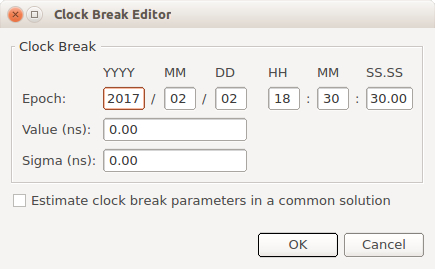
\includegraphics[width=0.35\textwidth]{stnedit-cbe.jpg}
  \end{center}
  \caption{Station clock break parameters edit window.}
  \label{fig-stnedit-cbe}
\end{figure}

The second approach consists in applying piecewise-continuous function to clocks
of a station. The parameters of the function are estimated in a separate
solution. Breaks between steps of the function absorb the effect of
clock breaks. Currently, only an offset is used in the clock break
function. In contrast to the previous approach, it requires the
determination not only of the approximate epoch of the clock break, but,
also its magnitude.
   On the other hand, in some rare cases, when a station has multiple clock
breaks over short intervals, it allows such observations to be used in
the data analysis.

The clock break editor is invoked when a user clicks the {\sl Add} or
{\sl Edit} button in the widget group {\sl List of Clock Break
Events} (see above). The edit window, Fig.~\ref{fig-stnedit-cbe},
allows a user to add or edit the epoch of the clock break (year, month,
day, hour, minute and second) and the its magnitude. The checkbox
{\sl Estimate clock break parameters in a common solution} switches the
type of a clock break. A user can modify a type of a particular clock
break, it is ok for the software to have different types of clock breaks
for one session.


%
%\begin{figure}[htb!]
%  \begin{center}
%    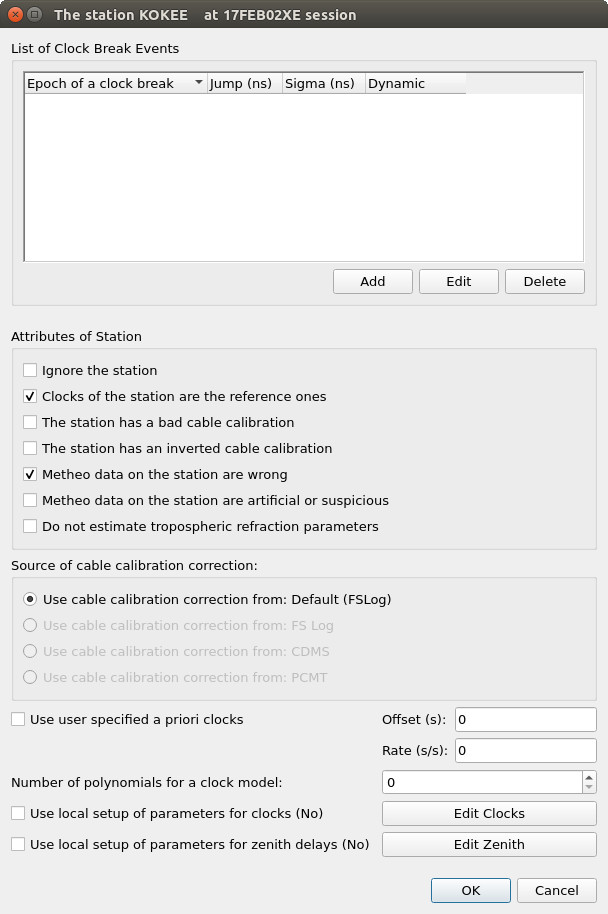
\includegraphics[width=0.3\textwidth]{stnedit-general.jpg}
%    \hspace{1cm}
%    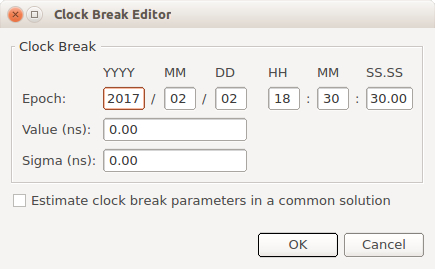
\includegraphics[width=0.3\textwidth]{stnedit-cbe.jpg}
%  \end{center}
%  \caption{Station attributes (left) and clock break parameters (right) edit windows.}
%  \label{fig-stnedit}
%\end{figure}
%




%
\subsection{Tab <<Sources (List)>>}
\label{subsect-sessedit-sources-list}

\begin{figure}[htb]
  \begin{center}
    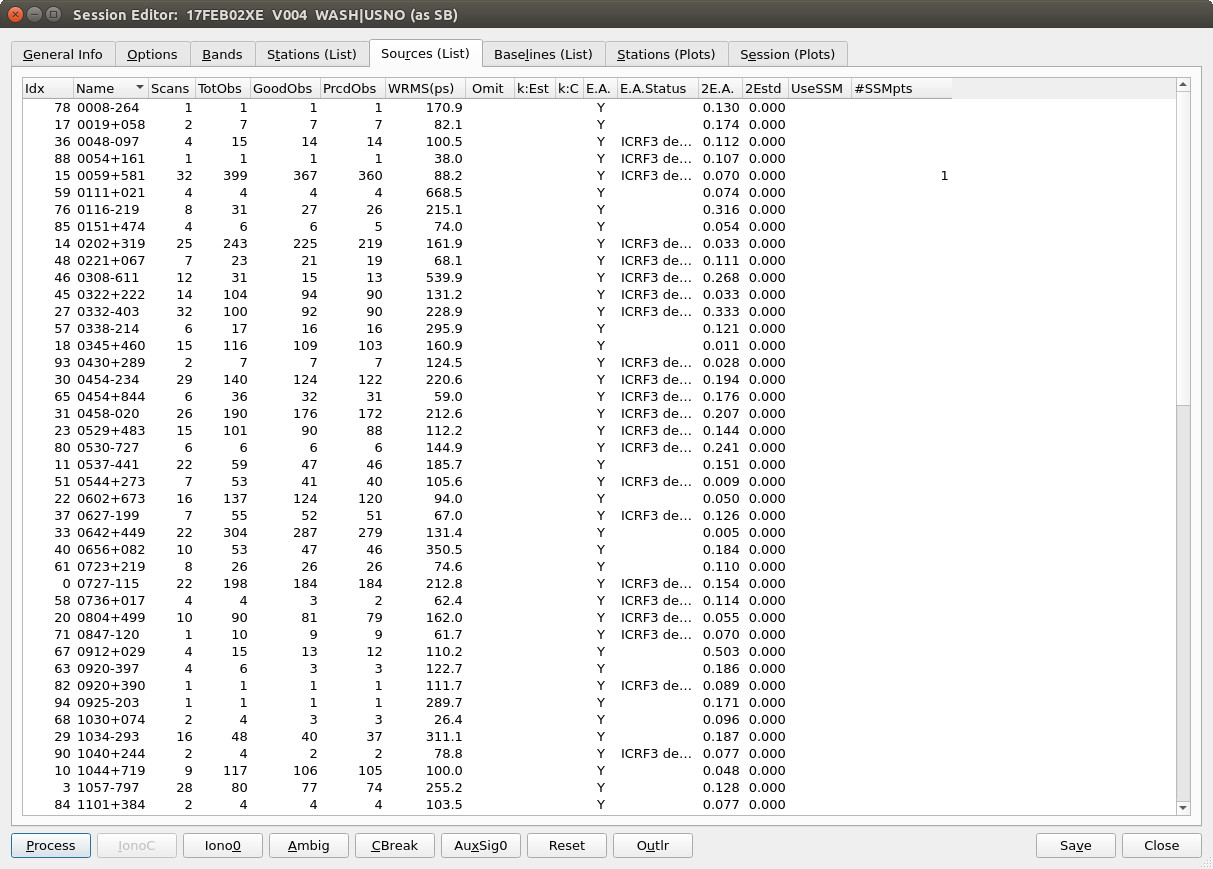
\includegraphics[width=1.0\textwidth]{sessedit-sources.jpg}
  \end{center}
  \caption{Session Editor window, list of sources.}
  \label{fig-sessedit-sources}
\end{figure}

The tab {\sl Sources (List)} shows the attributes of the sources that
were observed during a VLBI session. The list has the same organization
as the station list. The following source attributes are displayed: names
of sources are shown in the column {\sl Name}. The second column, {\sl Scans}, shows
total number of scans of a radio source. The column {\sl TotObs}
represents the total number of observations of a source. The numbers of
potentially good observations for each source are represent in the column
{\sl GoodObs}. The number of analyzed observations of a source is in the column {\sl PrcdObs}.
Residuals of the group or single band delays for the source are in the
{\sl WRMS(ps)} column.

In the same way as for the stations list, the user can exclude particular sources
from the analysis by clicking in the {\sl Omit} column. If the source is marked for
exclusion, the {\sl X} character will appear in the column.

The column {\sl k:Est} represents the "estimate the source position" attribute.
Again, as for stations, this flag does not turn on or off the estimation of source
coordinates.
%But it will be consulted by the software when a user tells it to estimate sources
%positions, and, if the flag is off, the coordinates of that particular source will be
%removed from a list of estimated parameters. 
It only tells whether a source's position will be estimated or not.
Now, by default, all sources are turned off from the estimation.

Also, a combination of estimated parameters may require applying constraints
for the estimated source positions (e.g., when positions of all available stations,
coordinates of sources and EOP are turned on). To select which source will
be included in No-Net-Rotations constraints click in the column {\sl k:C}
for the selected sources. The character {\sl *} will mark sources that will
be constrained.

Traditionally, interactive SOLVE and \nuSolve{} use source coordinates from
external a priori files. If a source is not present in such file, the a priori
values that were provided by CALC will be used. If the column {\sl E.A.}
contains a char "Y", the corresponding source is present in the a priori file.
The column {\sl E.A.Status} contains a comment string from the a priori file.

A length of arc between source a priori position that was
used by CALC and the value from the a priori file is displayed in the column
{\sl 2E.A.}. The units are milliarcseconds.

A length of arc between source a priori position and its estimated coordinates
(if source positions were estimated) is shown in the column {\sl 2Estd}.

The last two columns characterize use of a source structure model. The column
{\sl UseSSM} displays for which source the model should be applied (a character
<<Y>>). A number of secondary components of the model is shown in the column
{\sl \#SSMpts}. The section \emph{\ref{section-using-gui-ssm} Using a source structure model}
discuss details of the model application.



%%
%%------------------------------------------------------------------------
\subsubsection{Source Attributes Editor}
\label{subsubsect-sessedit-source-attr-edit}

A source attribute editor can be invoked by a double mouse click in the area
bounded by columns {\sl Idx} and {\sl Wrms(ps)}. In the same way as for a
station it allows a user to adjust available source attributes and edit
parameters of the source structure model
(see section \emph{\ref{section-using-gui-ssm} Using a source structure model} for details).

\begin{figure}[htb]
  \begin{center}
    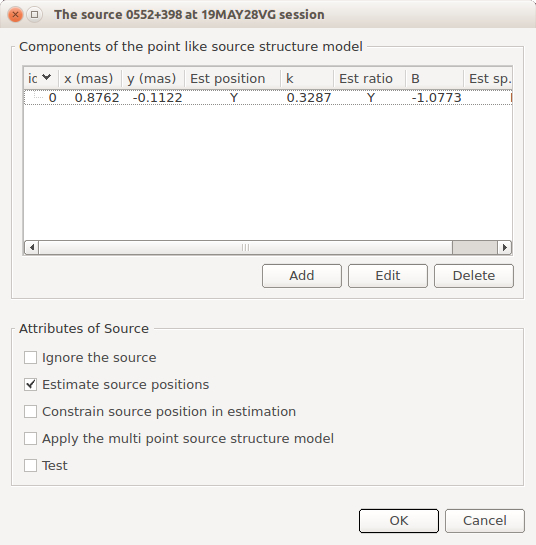
\includegraphics[width=0.35\textwidth]{srcedit-general.jpg}
  \end{center}
  \caption{Source attributes edit window.}
  \label{fig-srcedit-general}
\end{figure}

The upper group of widgets allows a user to edit the source structure
model. The group consists of the list of model components and three
buttons. If no model was defined for a specified source, the list will be
empty. To add a component of the model, click the {\sl Add} button and a
component editor window will appear (see next subsection).
To alter the parameters of a component, highlight it
in the list and press the {\sl Edit} button. The last
button, {\sl Delete}, removes a selected component from the list.

The lower group represents all available source attributes (they
can be altered by interacting with the source list too).


%%
%%------------------------------------------------------------------------
\subsubsection{Point like source structure model component Editor}
\label{subsubsect-sessedit-source-ssm-edit}

\begin{figure}[htb!]
  \begin{center}
    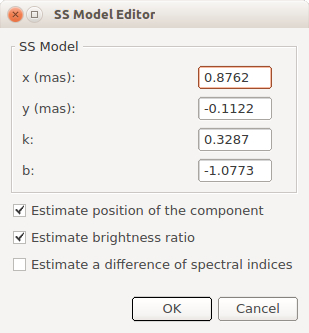
\includegraphics[width=0.35\textwidth]{srcedit-ssm.jpg}
  \end{center}
  \caption{Source structure model edit window.}
  \label{fig-srcedit-ssm}
\end{figure}


The component editor of the point like source structure model is a simple
window that allows a user to provide a relative position of a component
({\sl x(mas)} and {\sl y(mas)} fields), ratio of component brightness
with respect to the central component, {\sl k}, and a difference
of spectral indices, {\sl b}.

A user can specify which parameters of the source structure model
should be estimated. The corresponding check boxes are provided for
this purpose.



%%%%%%%%%%%%%%%%%%%%%%%%%%%%%%%%%%%%%%%%%%%%%%%%%%%%%%%%%%%%%%%%%%%%%%%%%%%%%%
\subsection{Tab <<Baselines (List)>>}
\label{subsect-sessedit-baselines}

\begin{figure}[htb!]
  \begin{center}
    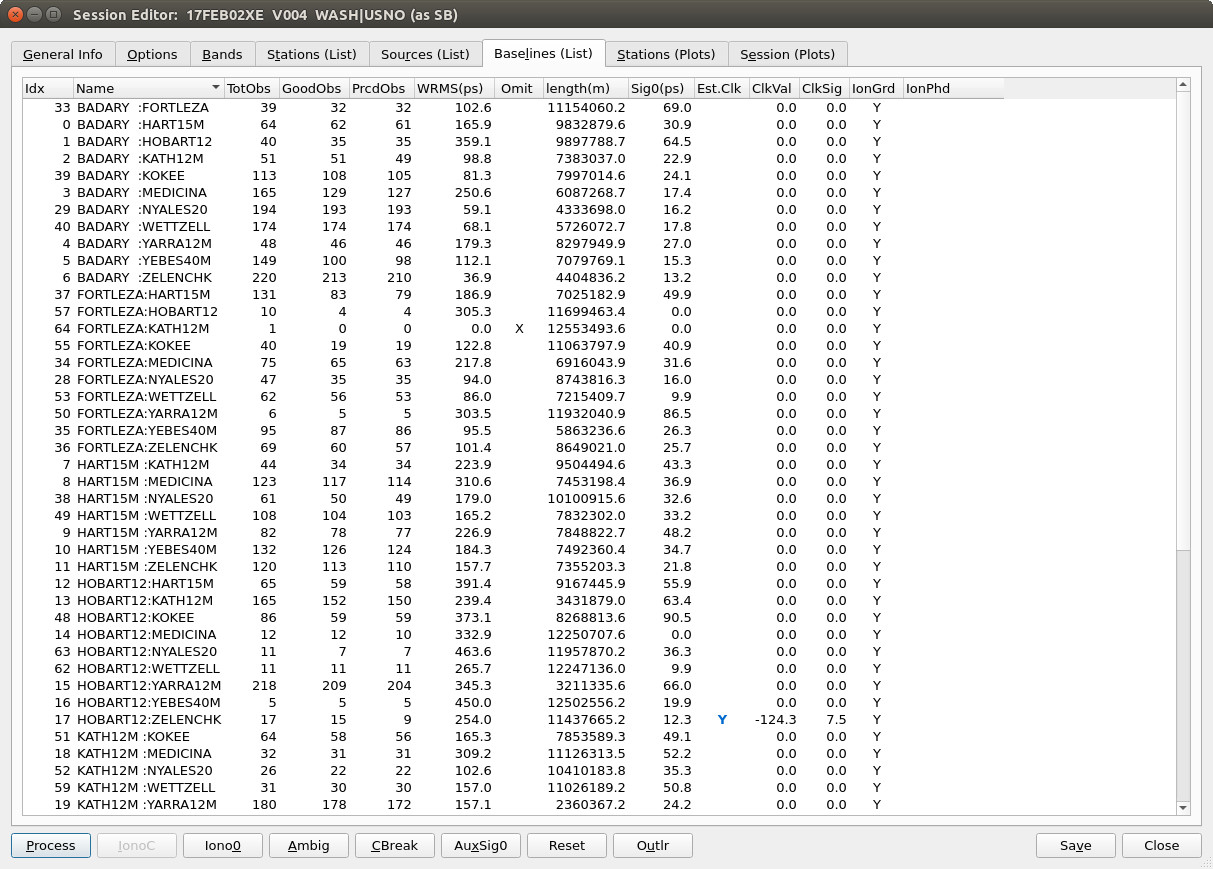
\includegraphics[width=1.0\textwidth]{sessedit-baselines.jpg}
  \end{center}
  \caption{Session Editor window, list of baselines.}
  \label{fig-sessedit-baselines}
\end{figure}

The tab {\sl Baselines (List)} displays the attributes of the baselines.
As for the previous two tabs, it includes statistical information: the
baseline name, total, good and processed numbers of observations, residuals.
Also, the column {\sl Omit} allows a user to deselect some particular
baseline from the solution. The next two columns display a length of a
baseline (meters) and correction of weights ({\sl Sig0(ps)}) for delays.

The column {\sl Est.Clk} marks baselines where clock offsets need
to be estimated. Depending on the procedures performed by the
correlator, there are cases when a baseline can have a constant clock
offset with respect to other baselines (i.e., triangles do not close).
To deal with such cases, CALC/SOLVE and \nuSolve{} adds an additional
parameter, a baseline clock offset. A mouse click in this column turns
on the estimation of the offset for the baseline. The character {\sl Y}
means <<on>>. By default, when a new VLBI session is read in, this flag
is <<off>> for all baselines. But when a previously processed session is
read in (e.g., version 4 of the Mk-3 DBH format), the flags are set
according to the baseline clock information stored in the database.

In general, the need for baseline clock offset estimation is relatively
rare. At the Goddard we apply the following procedure to the baseline
clock offset. First, after all detected anomalies (clock breaks,
ambiguities, outliers, etc.) are resolved, then baseline clock offsets
are added to the list of the estimated parameters. Then, all baseline
clock offsets with values less than three times their standard
deviations are removed and the estimation process is repeated. We also
do not estimate baseline clock offsets for baselines with a small number
of good observations (say, less than $10$ points) and for offsets where
the estimated values are very small (e.g., less than $10ps$). After
reweighting and outlier elimination are performed, we will repeat the
check of baseline clock offset values. As a result, baseline clock
offsets are usually estimated for only a few baselines.

The columns {\sl ClkVal} and {\sl ClkSig} show offsets and theirs
standard deviations (in picoseconds) for baselines which clocks offsets
were estimated in the last solution.

To make the process of selection of the baseline clock offsets faster,
the symbols {\sl Y} in the column {\sl Est.Clocks} are colored (see
Fig.~\ref{fig-sessedit-baselines}). The red color means that the
absolute value of the estimate is less than its standard deviation. The
orange color means that the estimate is greater than one but less than
three standard deviations. The black color indicates that the estimated
offset is greater than three standard deviations, but less than $10ps$,
or was not estimated yet. And the blue color means that the estimation
is significant.

The columns {\sl IonGrd} and {\sl IonPhd} represent flags of taking into
account ionospheric corrections (if available) for the group and the phase
delays. By default, we use the ionosphere corrections for the group delays.
If you are not sure, keep it as is.


\subsubsection{Baseline Attributes Editor}
\label{subsubsect-sessedit-baselines-blneditor}
A double mouse click in the area bounded by columns {\sl Idx} and {\sl
Sigma\_0} invokes a baseline attributes editor window (see
Fig.~\ref{fig-blnedit-general}). This window allows a user to turn
<<on>> or <<off>> all available baseline attributes and set a value of
additional weight manually for the baseline.

\begin{figure}[htb!]
  \begin{center}
    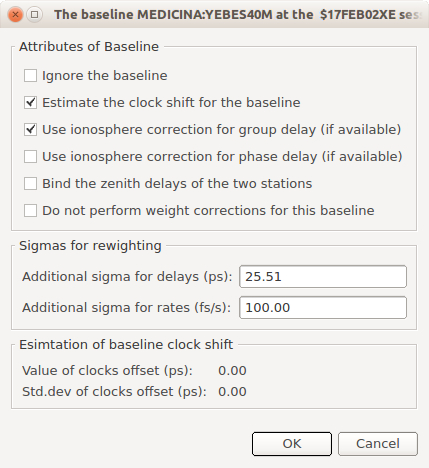
\includegraphics[width=0.35\textwidth]{blnedit-general.jpg}
  \end{center}
  \caption{Baseline attributes edit window.}
  \label{fig-blnedit-general}
\end{figure}

The baseline attributes editor window allows to alter the additional
sigma for the group delay and delay rates. Also, it displays the
estimated baseline clock offset and its standard deviations.

The checkbox {\sl Bind the zenith delays of the two stations} is for
tests purposes, do not turn it <<on>>.

%Again, do not turn <<on>> the checkbox {\sl Bind the zenith delays of the two
%stations}, this option is for tests purposes.

If the last check box, {\sl Do not perform weight corrections for this baseline},
is checked on, observations obtained on this baseline will not be used
in a procedure of weight corrections to have $chi^2=1$. The values of
the additional weights, if they are not zeros, will be applied in data analysis.


%
\subsection{Tab <<Stations (Plots)>>}
\label{subsec-stations-plots}
The tab {\sl Stations (Plots)} displays various station dependent data
from either measurements or estimations. The Fig.~\ref{fig-sessedit-stations-p}
shows an example of cable calibrations as a function of time.


\begin{figure}[htb!]
  \begin{center}
    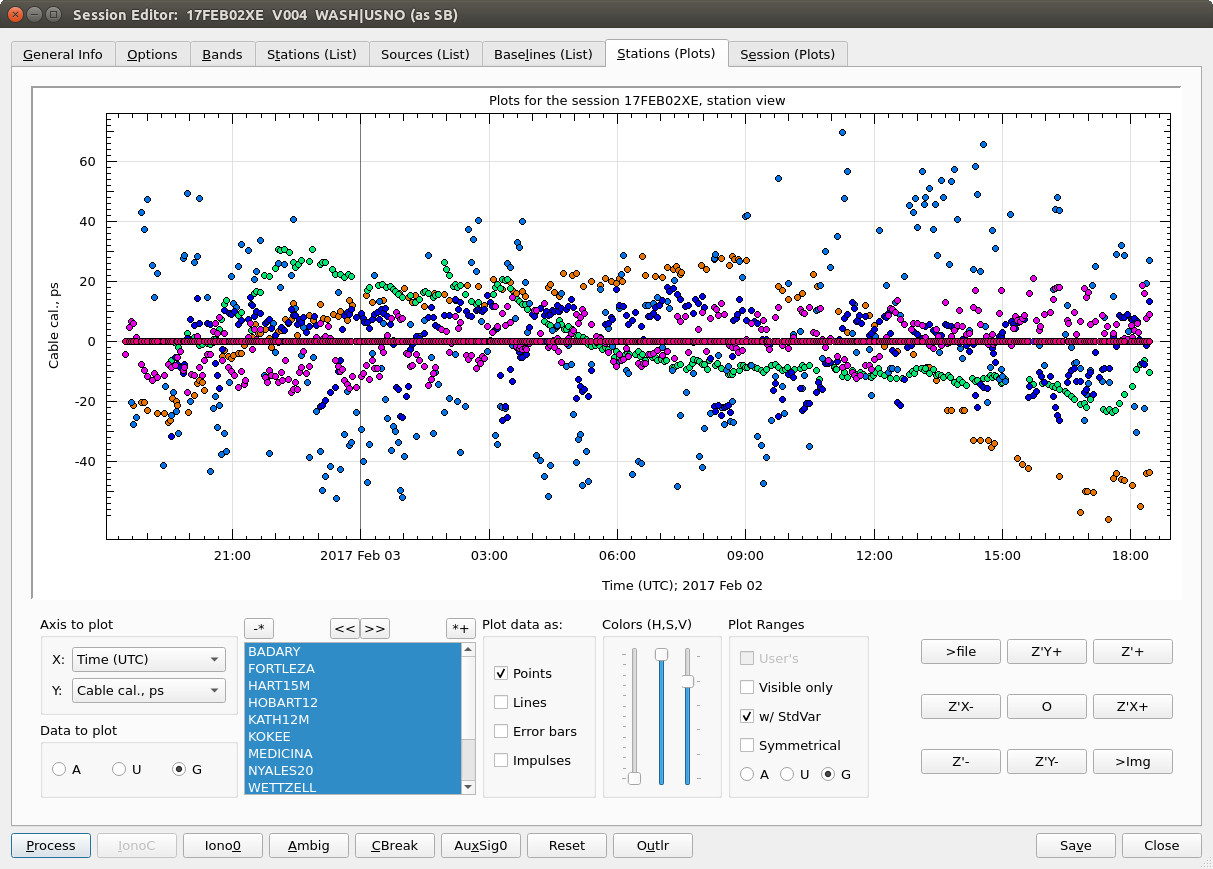
\includegraphics[width=1.0\textwidth]{sessedit-stations-p.jpg}
  \end{center}
  \caption{Session Editor window, station dependent plots: cable calibration data.}
  \label{fig-sessedit-stations-p}
\end{figure}

Currently the following measurements are displayed: cable calibration
values (if different types of cable calibrations are available, they are
plotted as separate data), meteorological parameters (atmospheric temperature, 
pressure and
relative humidity) and antenna pointing (azimuth and elevation, parallactic angle). In
addition, the following estimations and their standard deviations are
displayed: model of clock function (if time-varying parameters were
estimated, e.g., PWL function or stochastic parameters, then polynomial
model is not shown), zenith delay and its gradients. Also, a total
zenith delay is displayed on this plot.


%
\subsection{Not used observation window}
\label{subsec-not-used-obs}
The Session Editor window is capable to list observations that are not
in a solution. There are two groups of such observations: unusable
and deselected observations. The first group are observations that
have either quality code that is lower than the threshold or a source,
a station or a baseline has been deselected. Also, in some rare cases,
when an observation has only one good channel it will be considered as
unusable too.


\begin{figure}[htb!]
  \begin{center}
    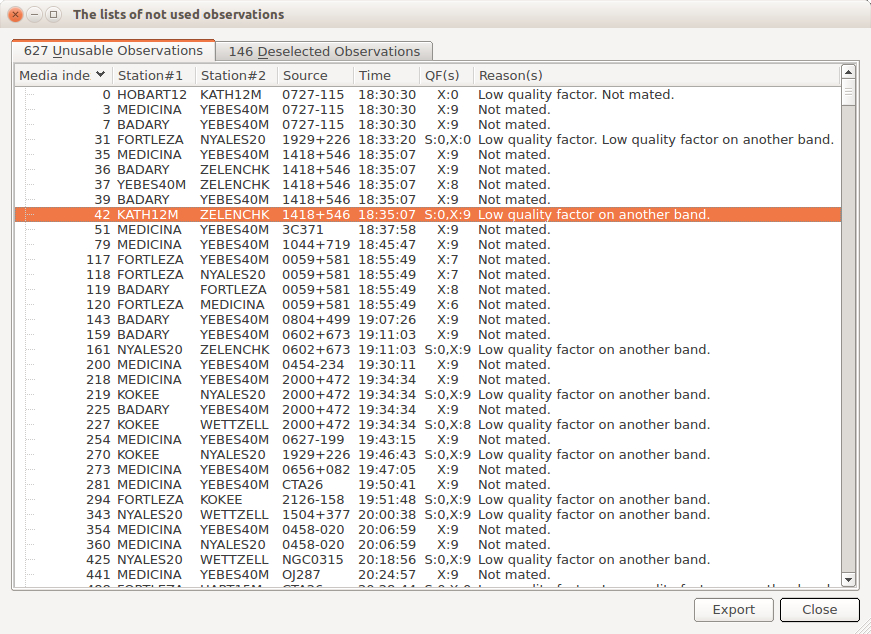
\includegraphics[width=1.0\textwidth]{sessedit-nonused-obs-unusable.jpg}
  \end{center}
  \caption{A list of observations that are not in a solution: unusable observations.}
  \label{fig-sessedit-nonused-obs-unusable}
\end{figure}

\begin{figure}[htb!]
  \begin{center}
    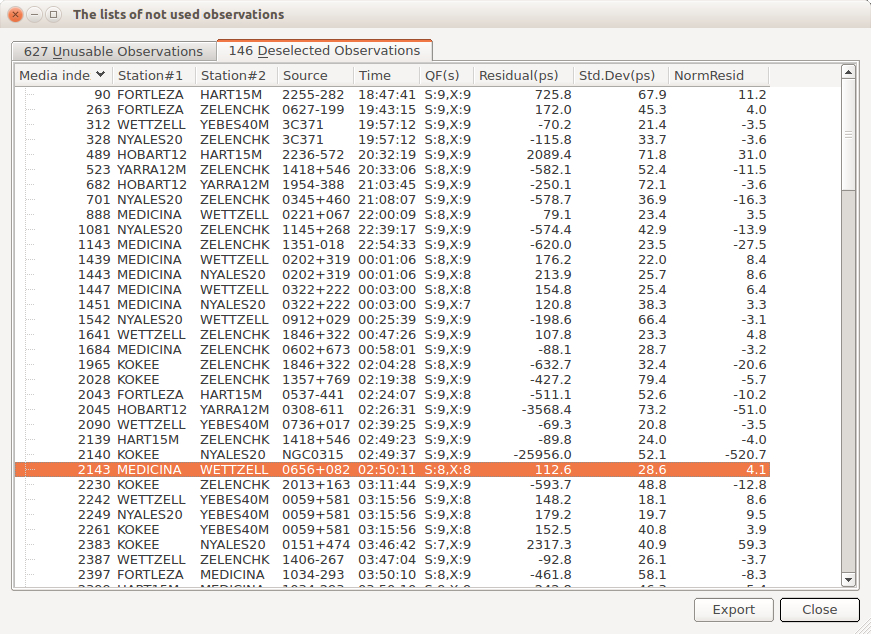
\includegraphics[width=1.0\textwidth]{sessedit-nonused-obs-deselected.jpg}
  \end{center}
  \caption{A list of observations that are not in a solution: deselected by a user observations.}
  \label{fig-sessedit-nonused-obs-deselected}
\end{figure}

The last group of observations are the observations that were explicitly marked
for deselection either by a user or the outlier processing procedure.

At any stage of data analysis a user can press a key combination {\sl Ctrl+i}
to invoke {\sl Not used observation} window, see
Figs.~\ref{fig-sessedit-nonused-obs-unusable}--\ref{fig-sessedit-nonused-obs-deselected}.
The window has two tabs, each for each type of not used observations.

The first tab, {\sl Unusable Observations}, displays a list of unusable
observations -- station and source names, time of observation, quality
factors and a reason why the observation cannot be used. The list can be
sorted by content of each column with left mouse click on a header of
a column.

The second tab, {\sl Deselected Observations}, lists observations that
were explicitly removed from a solution. In addition to station and
source names and quality factors, the list displays residuals of delays,
their standard deviations and the corresponding normalized residual of
deselected observation.

The software is capable to save the list of observations with indication
of their usability and residuals as an ASCII file. Such file is designed to
be used by external utilities, like {\sl anl\_comments}, and are generated
automatically when a user press {\sl Save} button of the {\sl Session Editor}
window. To create the file manually, a user can click the button {\sl Export}
of the {\sl Not used observation} window. The file will be written in the
directory specified by the field {\sl List of not used observations output}
of the software Preferences (see the section \ref{prefs-general}).






%%%%%%%%%%%%%%%%%%%%%%%%%%%%%%%%%%%%%%%%%%%%%%%%%%%%%%%%%%%%%%%%%%
%
%
%
%
\chapter{Selected practical issues of using \nuSolve{} in a GUI mode}
\label{chapter-using-gui-mode}



%%%%%%%%%%%%%%%%%%%%%%%%%%%%%%%%%%%%%%%%%%%%%%%%%%%%%%%%%%%%%%%%%%
%
%
%
%
\section{Processing a regular VLBI session}
\label{sect-processing-a-session}
In this section we overview the operations necessary to analyze a
regular 24-hour VLBI session. In general, we start with simple
parameterization, only clock shifts and rates, and perform an analysis
of the single band delays. At this stage we check for possible clock
breaks at stations. Then, we process to the group delays to resolve
2$\pi$ ambiguities and, again, possible effects that look like clock
breaks. Before ambiguities and clock breaks are resolved, there is no
sense in estimating other parameters except the polynomials of the clock
functions.

When these two phenomena, clock breaks and unresolved ambiguities are
fixed, we add zenith delays and station positions to the list of
estimated parameters and check for outliers. Also, we calculate
ionospheric corrections.

Time-varying models of clock and tropospheric parameters are introduced
in the last stage. Also, other parameters are added: the rate of Earth
rotation, angles of nutation, and baselines clock offsets. At this stage
we also do a reweighting of the observations and process the outliers.
The last two operations are performed in conjunction.

\begin{figure}[htb!]
  \begin{center}
    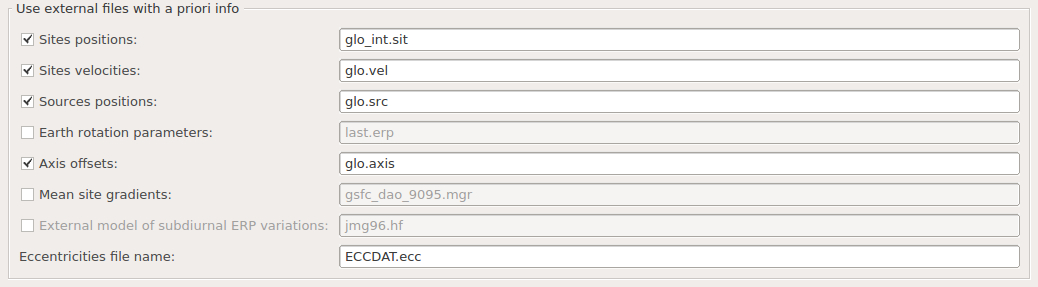
\includegraphics[width=.95\textwidth]{example-begin-apriori.jpg}
  \end{center}
  \caption{GUI: use of external {\it a~priori} files.}
  \label{fig-ex-begin-apriori}
\end{figure}

Before you make any analysis, verify that you have all the necessary
files with {\it a~priori} data. Check the tab {\sl Options}, the subtab
{\sl External a priori and models}, Fig.~\ref{fig-ex-begin-apriori}. If
you do not have the files, turn the corresponding checkboxes <<off>>.
Some of the files can be obtained from
$$
%http://gemini.gsfc.nasa.gov/solve\_save
%https://vlbi.gsfc.nasa.gov/software\_calc\_solve\_auxiliary.htm
%ftp://cddis.gsfc.nasa.gov/pub/vlbi/gsfc/ancillary/solve_apriori
https://cddis.nasa.gov/archive/vlbi/gsfc/ancillary/solve\_apriori/
$$
It is recommended to use the {\it a~priori} files at least for station
positions, station velocities and source coordinates. Also, keep
information in these files updated, it will save you time.



%
%
%%%%%%%%%%%%%%%%%%%%%%%%%%%%%%%%%%%%%%%%%%%%%%%%%%%%%%%%%%%%%%%%%%%%%%%%%%%%
%%
%%
%%
%%%%%%%%%%%%%%%%%%%%%%%%%%%%%%%%%%%%%%%%%%%%%%%%%%%%%%%%%%%%%%%%%%%%%%%%%%%%
\subsection{Reading the session and preparing for processing}
For a demonstration of data analysis we use IVS-R4 session 13SEP05XE.
This is a regular VLBI session, it has one clock break effect at SVETLOE in
the S-band and mixed value of ambiguity spacings in the S-band.
The clock break effect is caused by applied manual phase calibration in
two parts.

First, the user has to read the session into \nuSolve{}. If the session
is in the database format, two files (S- and X-band) are expected.

\begin{figure}[htb!]
  \begin{center}
    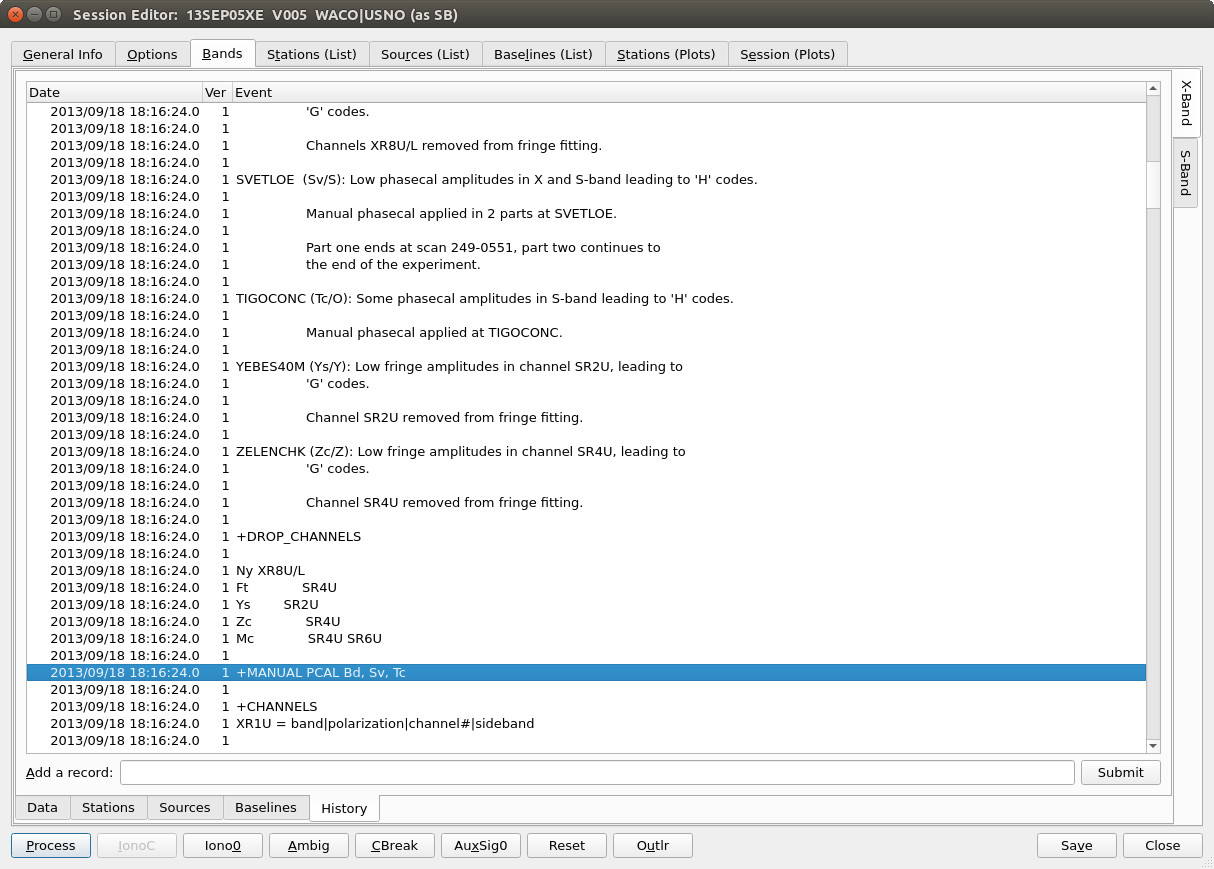
\includegraphics[width=1.0\textwidth]{example-begin-hist.jpg}
  \end{center}
  \caption{The session 13SEP05XE: the history records.}
  \label{fig-ex-begin-hist}
\end{figure}


After the files are imported and the Session Edit window has appeared on the
screen, check the history part of the session (preferable the X-band),
see Fig.~\ref{fig-ex-begin-hist}. To do so, select the {\sl Bands} tab of the
Session Editor and then select the {\sl History} tab of the X-band.

The highlighted text on the figure history record says:
\begin{verbatim}
+MANUAL PCAL Bd, Sv, Tc
\end{verbatim}
It is a part of the correlator report and means that manual phase calibration
was applied for BADARY, SVETLOE and TIGOCONC. Also, the correlator
comments on station performance are in a section above this record.

Normally if the correlator applied manual phase calibration, we should not use
the cable calibration data. On the tab {\sl Stations (List)}, Fig.~\ref{fig-ex-begin-stations},
we deselect the use of cable calibration data for these stations.
Also, KOKEE is known to have incorrect cable calibration measurements,
so for this station use of the cable calibration data is turned off too.

\begin{figure}[htb!]
  \begin{center}
    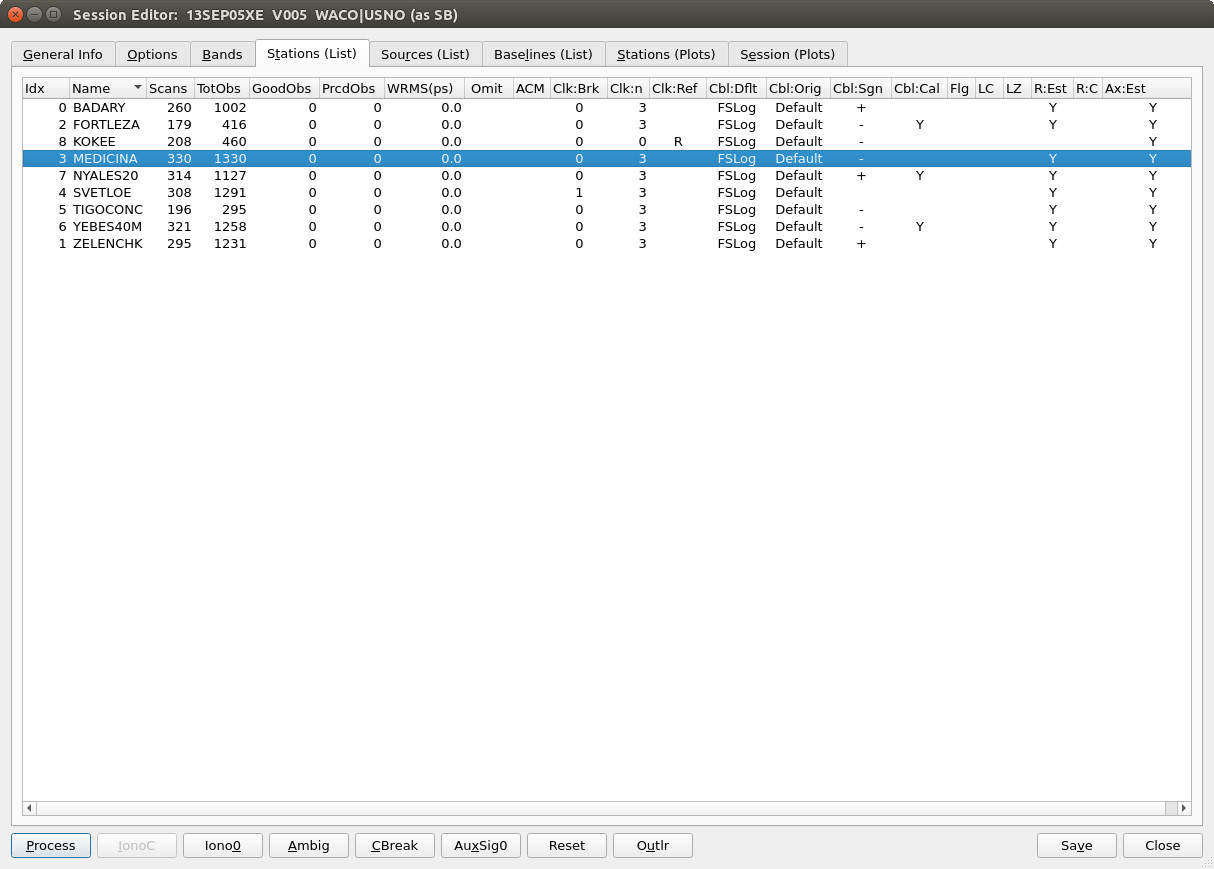
\includegraphics[width=1.0\textwidth]{example-begin-stations.jpg}
  \end{center}
  \caption{The session 13SEP05XE: attributes of the stations.}
  \label{fig-ex-begin-stations}
\end{figure}

If the checkbox {\sl Perform set up of the session} of the configuration
tab {\sl Post import actions} is <<on>> for a network of the session
(see subsection~\ref{subsect-config-pia}), \nuSolve{} will check the
history records and will turn off the cable calibrations automatically
for these stations (in this case you can see a note in the log, as it shown on 
Fig.~\ref{fig-ex-begin-log}). Since there is no fixed format of reporting use of
manual phase calibrations and correlator reports are written by humans,
the procedure of analysis of history records can misinterpret the
records and assign a wrong flag for a wrong station. We would suggest to
check history records manually even if the procedure of session setup is
scheduled after the data were read.

\begin{figure}[htb!]
  \begin{center}
    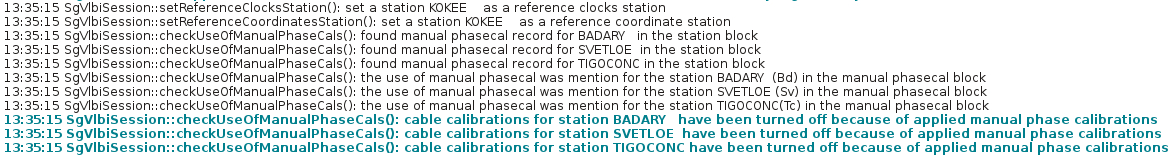
\includegraphics[width=1.0\textwidth]{example-begin-log.jpg}
  \end{center}
  \caption{The session 13SEP05XE: part of the log, \nuSolve{} detected manual
  phase calibration for BADARY, SVETLOE and TIGOCONC and turned off the use
  of cable calibrations for these stations.}
  \label{fig-ex-begin-log}
\end{figure}

We chose KOKEE as the reference clock station. We set the number of its
polynomial terms to zero (in this case the clock parameters will not be
estimated at all) and set the flag {\sl Clk:Ref} (a station with this
flag will be declared a <<reference clock station>> in the output,
database or vgosDb format; also, if the number of polynomial model is
not set to zero, a constraints will be applied to the clock parameters
of the station) for the station, see Fig.~\ref{fig-ex-begin-stations}.
Also, for station NYALES20 the flag "Estimate position" is not set, we
consider it to be the reference station.

Before processing the session, check the data collected at the stations,
{\sl Stations (Plots)} tab of the Session Editor. For this session
there is a break in the cable calibration data for MEDICINA, see
Fig.~\ref{fig-ex-begin-stations-cables}.

\begin{figure}[htb!]
  \begin{center}
    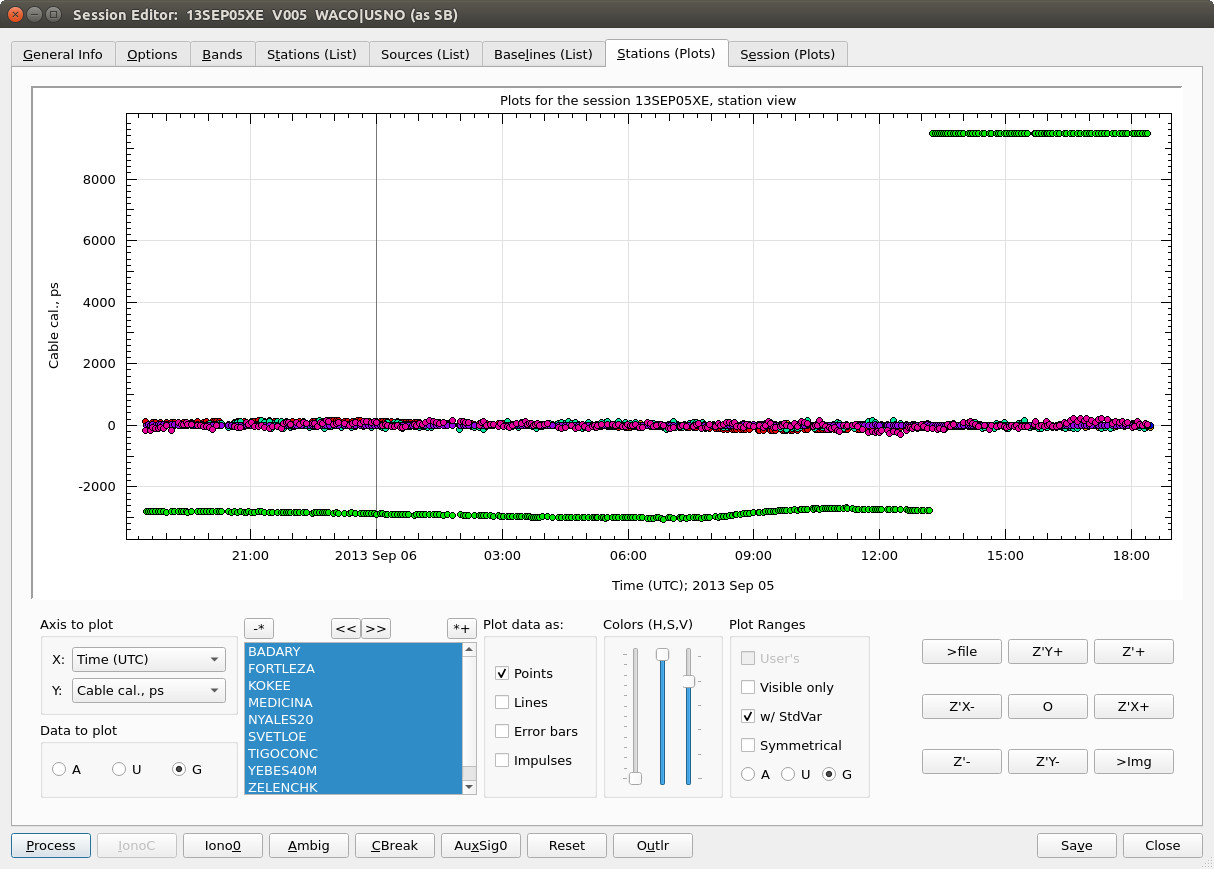
\includegraphics[width=1.0\textwidth]{example-begin-stations-cables.jpg}
  \end{center}
  \caption{Session 13SEP05XE: cable calibrations data.}
  \label{fig-ex-begin-stations-cables}
\end{figure}

Such effects are relatively rare and, sometimes reflect actual cable
behavior. To figure out is this is a real change in cables or some
artificial effect, we need to make an analysis of the session and check
for residuals of station MEDICINA. If there is a clock break of about
$12ns$ when the MEDICINA cable calibrations are applied, then we would
need to tun off the cable calibration data for this station.



%
%
%%%%%%%%%%%%%%%%%%%%%%%%%%%%%%%%%%%%%%%%%%%%%%%%%%%%%%%%%%%%%%%%%%%%%%%%%%%%
%%
%%
%%
%%%%%%%%%%%%%%%%%%%%%%%%%%%%%%%%%%%%%%%%%%%%%%%%%%%%%%%%%%%%%%%%%%%%%%%%%%%%
\subsection{Processing single band delay}
To obtain a solution, press the {\sl Process} button at the bottom of
the Session editor. By default, we begin data analysis using the single
band delays. If the user did not switch to another type of observables,
a single band delay solution will be obtained using a simple model --
only clock offsets and rates will be estimated. To see the results of
this solution switch to residuals, the tab {\sl Bands}, subtab {\sl
Data}, see Fig.~\ref{fig-ex-pass-01}.

\begin{figure}[htb!]
  \begin{center}
    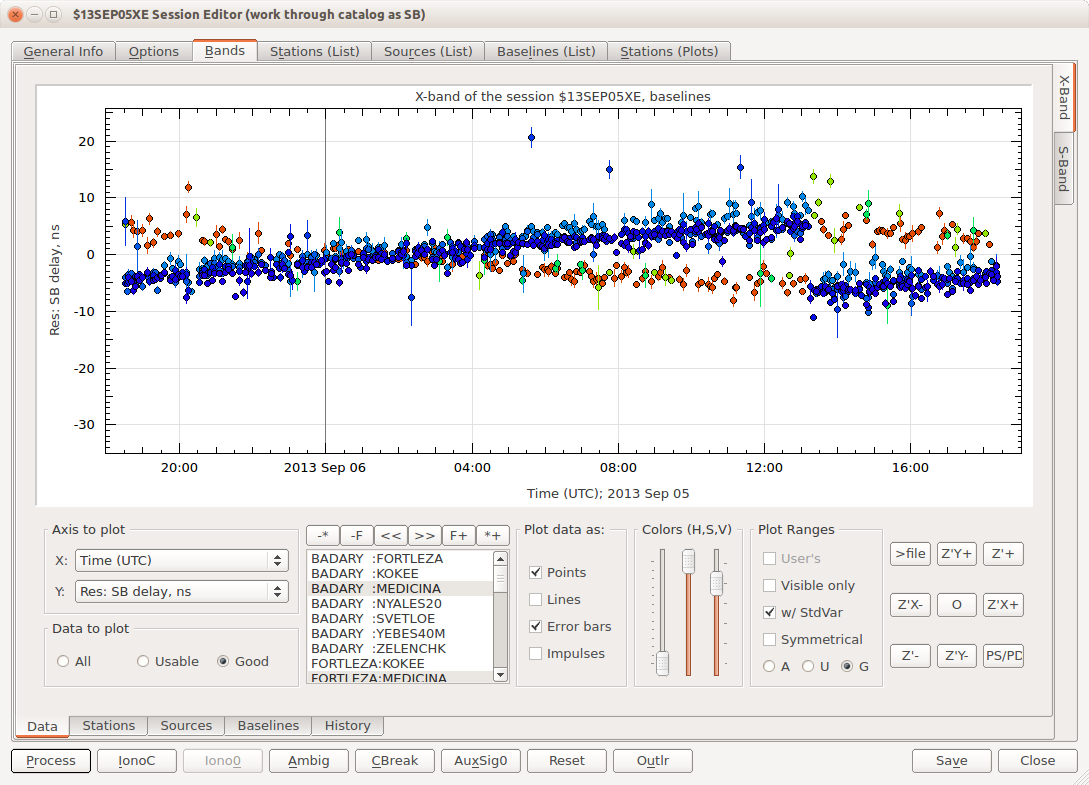
\includegraphics[width=1.0\textwidth]{example-pass-01.jpg}
  \end{center}
  \caption{Session 13SEP05XE: single band delay residuals.}
  \label{fig-ex-pass-01}
\end{figure}

On these plots only the residuals for MEDICINA are displayed. As one can
see, there is an expected clock break, so we need to turn off the use of
cable calibration for MEDICINA. Switch to {\sl Stations (List)} and
turn off the proper flag. Repeating the estimation of clocks shows that
there is no longer a visible clock break for MEDICINA after the cable
calibration is turned off.

Since the single band delay residuals do not reveal any other clock
break effects, we can switch to the group delays and continue the
analysis. At the {\sl Band} tab of the window, select the {\sl Data}
tab, then click on the combobox of the {\sl Y} axis in the {\sl Axis
to Plot} group of the plotter. Select the {\sl Res: GR delay, ns}
option to plot the group delay residuals (see
Fig.~\ref{fig-ex-pass-02}).

\begin{figure}[htb!]
  \begin{center}
    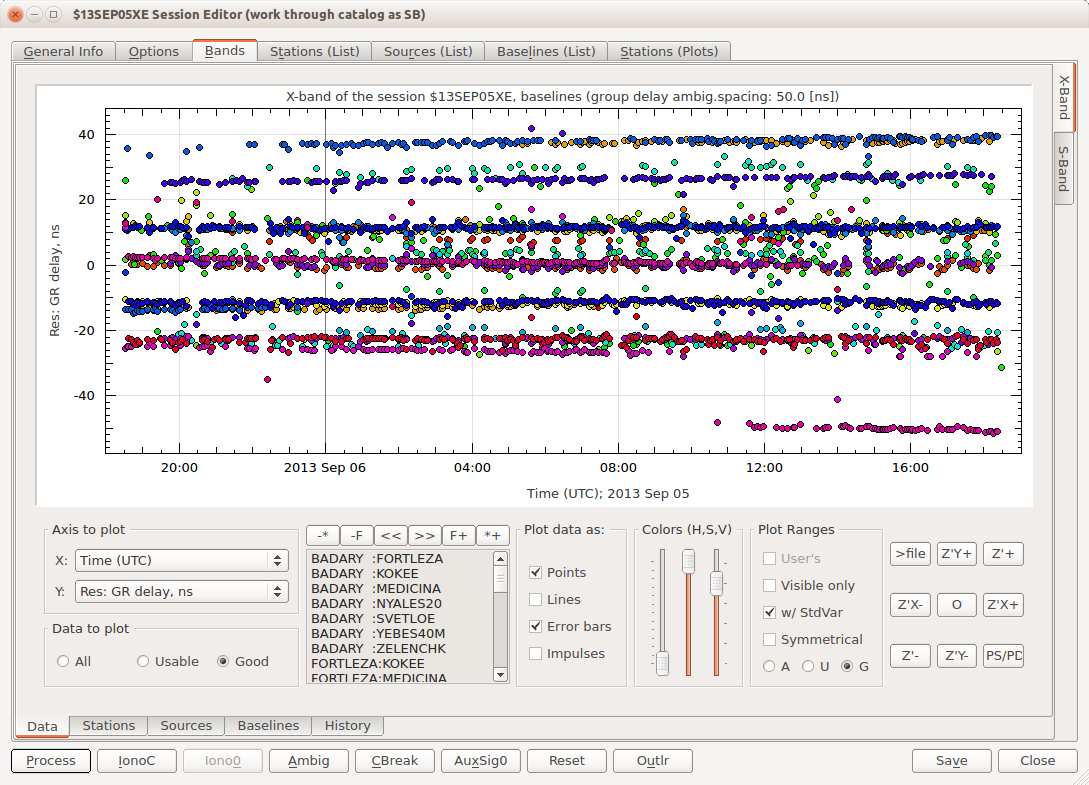
\includegraphics[width=1.0\textwidth]{example-pass-02.jpg}
  \end{center}
  \caption{Session 13SEP05XE: group delay residuals.}
  \label{fig-ex-pass-02}
\end{figure}

On the plot one can see the group delay residuals calculated using a
solution for the single band delays. Differences from these two
observables are caused by contribution from the ionosphere and
unresolved ambiguities. If you add lines to the plots (checkbox {\sl
Lines} in the group {\sl Plot data as} of the plotter) or display
each baseline one by one, you can see the effect of the unresolved
ambiguities.


%
%

% Start of KDB ------------------------------------
%%%%%%%%%%%%%%%%%%%%%%%%%%%%%%%%%%%%%%%%%%%%%%%%%%%%%%%%%%%%%%%%%%%%%%%%%%%%
%%
%%
%%
%%%%%%%%%%%%%%%%%%%%%%%%%%%%%%%%%%%%%%%%%%%%%%%%%%%%%%%%%%%%%%%%%%%%%%%%%%%%
\subsection{Resolving ambiguities}
\label{subsect-resolving-subambiguities}
\nuSolve{} has two modes for fixing the ambiguities -- manual and
automatic. In the manual mode, a user marks one or more points and
presses either the {\sl ``-''} key or the {\sl ``=''} key to adjust ambiguity
multipliers. To invoke the automatic mode, press the {\sl Ambig} button
of the Session Editor window. Usually, the automatic mode should be used
to resolve the ambiguities, and adjustments should be made using the
manual mode when it is necessary.

The group delay ambiguities have to be resolved for each band separately
and before including the ionosphere corrections for the group delays.

So, press the button to resolve the ambiguities. Then make a new
solution. The residuals for the X-band will be in the range of $20ns$,
which is smaller than the ambiguity spacing. After that, switch to the
S-band (select the tab {\sl S-Band} in the top right part of the
window) and repeat the procedure. For the S-band, the scatter is usually
much bigger. Also, it often happens that, due to lost channels at one or
more stations, the ambiguity spacing can vary depending on the stations
that form a baseline. The typical value of the ambiguity spacings for each
baseline is showed on {\sl Baselines} tab in the bottom of the tab {\sl Bands}.

A left mouse button click on the header {\sl Ambig.Spc} of the {\sl Baselines}
tab sorts the column in numerical order, Fig~\ref{fig-ex-pass-021}.
For our session the baseline MEDICINA:YEBES40M has ambiguity spacing
equal to $25ns$, all other baselines with MEDICINA as well as the
baselines with FORTLEZA and ZELENCHK have ambiguity spacings of $50ns$,
and all remaining baselines have ambiguity spacings of $100ns$.

\begin{figure}[tb]
  \begin{center}
    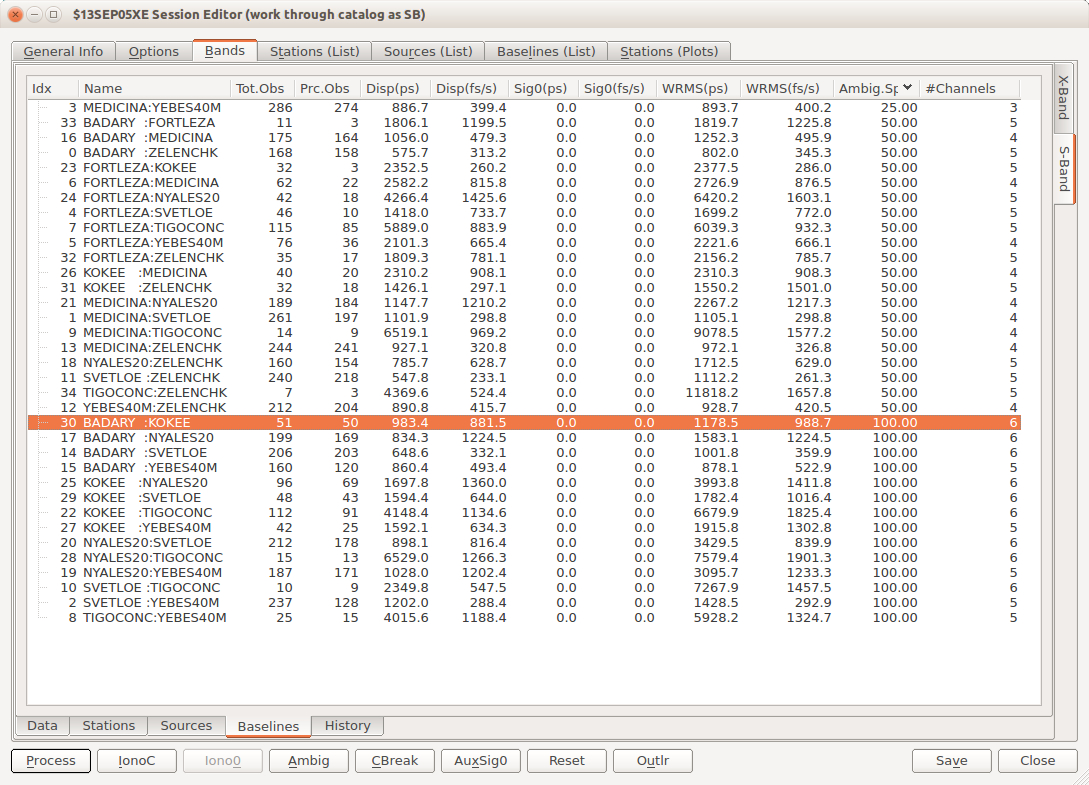
\includegraphics[width=1.0\textwidth]{example-pass-021.jpg}
  \end{center}
  \caption{Session 13SEP05XE: Ambiguity spacings on the S-band.}
  \label{fig-ex-pass-021}
\end{figure}

The combination of large scatter and small ambiguity spacing makes it hard
to resolve the ambiguities in automatic mode. You will need to repeat
the operation several times. If necessary, roll back to the single band
delay solution and repeat the operation or adjust ambiguities manually.

The following algorithm could help in complicated cases: turn off
stations with clock breaks; deselect all baselines but one of stations
which ambiguity spacings less than the nominal value (usually, keep
selected a baseline with the reference clock station). Resolve ambiguities.
Manually adjust ambiguities for deselected baselines -- on the plot
press {\sl -*} button, than highlight only one particular baseline,
turn on plotting all or usable observations (the radio button {\sl A}
or {\sl U} in the {\sl Plot Ranges} widget group).
%
%check the box {\sl All Data} 
%
and adjust the ambiguities manually for all observations of the baseline.
If everything
is ok, turn on the stations with clock breaks and resolve ambiguities
for these stations. It should be noted also, if a station is deselected,
all its baselines will be deselected too by the software. The software
deselects a station if all its baselines are deselected too. So, if you
turn on a station (on the {\sl Stations (List)} tab) you have to turn
on its baselines also (on the {\sl Baselines (List)} tab).

As one can see, the station SVETLOE has a clock break effect at S-band.
The reason for this break in the residuals is a manually applied phase
calibration that consists of two parts. There are records in the
correlator report (see the history part):

\begin{verbatim}
SVETLOE  (Sv/S): Low phasecal amplitudes in X and S-band leading to 'H' codes.

    Manual phasecal applied in 2 parts at SVETLOE.

    Part one ends at scan 249-0551, part two continues to
    the end of the experiment.
\end{verbatim}

After all ambiguities are resolved, the residuals should look like the
ones shown in Fig.~\ref{fig-ex-pass-03}. The clock break at SVETLOE is
clearly visible.

\begin{figure}[htb!]
  \begin{center}
    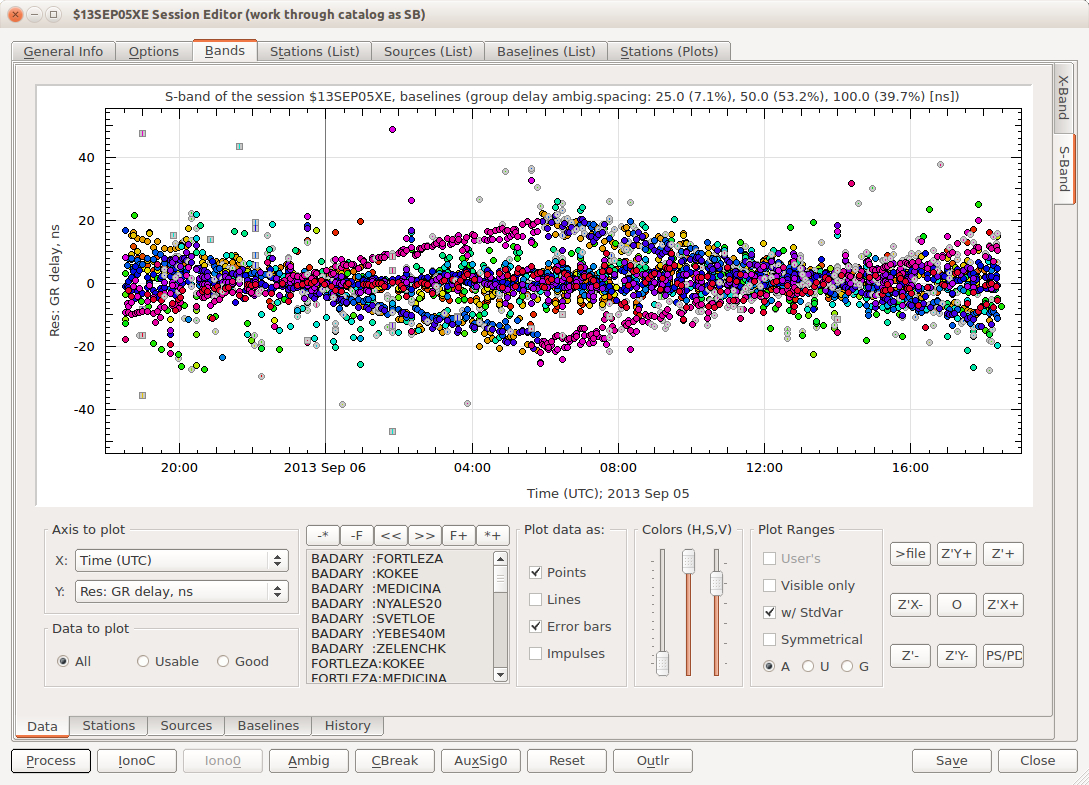
\includegraphics[width=1.0\textwidth]{example-pass-03.jpg}
  \end{center}
  \caption{Session 13SEP05XE: group delay residuals on the S-band.
           A clock break effect is on baselines of SVETLOE.}
  \label{fig-ex-pass-03}
\end{figure}


%
%
%%%%%%%%%%%%%%%%%%%%%%%%%%%%%%%%%%%%%%%%%%%%%%%%%%%%%%%%%%%%%%%%%%%%%%%%%%%%
%%
%%
%%
%%%%%%%%%%%%%%%%%%%%%%%%%%%%%%%%%%%%%%%%%%%%%%%%%%%%%%%%%%%%%%%%%%%%%%%%%%%%
\subsection{Processing a clock break}
\label{subsect-processing-clock-break}
In the software there are two approaches to take into account a clock
break. The first one is to estimate clock break magnitudes in a solution
(as interactive SOLVE does). The second approach is to add a stepwise
linear function to compensate for the break. Both approaches have their
own pluses and minuses. For the first type of clock breaks we do not need
to know a magnitude of the break, on the other hand, if a time interval
between two breaks is short, global SOLVE will fail to obtain a solution
due to high correlations.

The user can add a clock break to observations on one particular band or
to all data. Clock breaks that are set up for a band can be only of one
type, a stepwise linear function. Clock breaks that are applied to all
observations could be of both types. When the software adds a clock break
and the check box {\sl Estimate clock break parameters in common solution}
on the sub-tab {\sl Options --> General} is <<on>> (see section~\ref{sect-config-general}), then the clock break
will be added to whole session and will be of the second type.

\begin{figure}[htb!]
  \begin{center}
    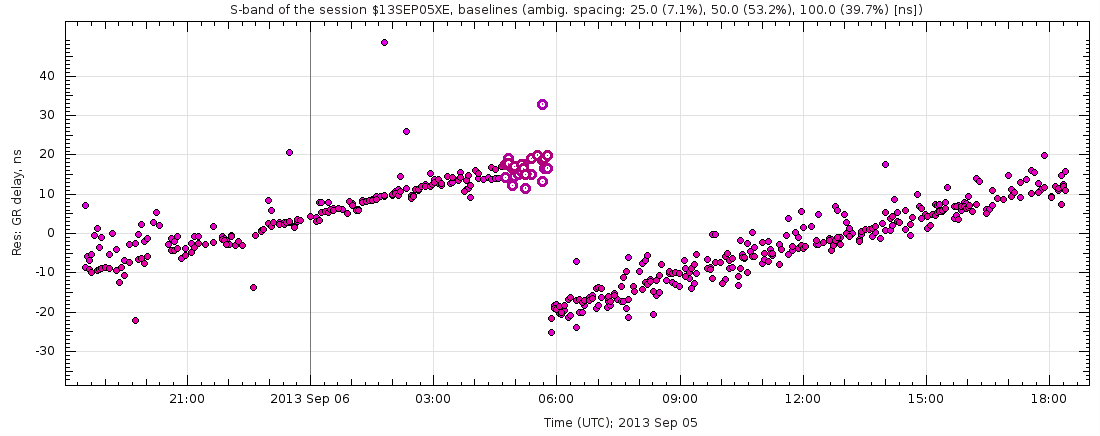
\includegraphics[width=.7\textwidth]{example-pass-04-1.jpg}
    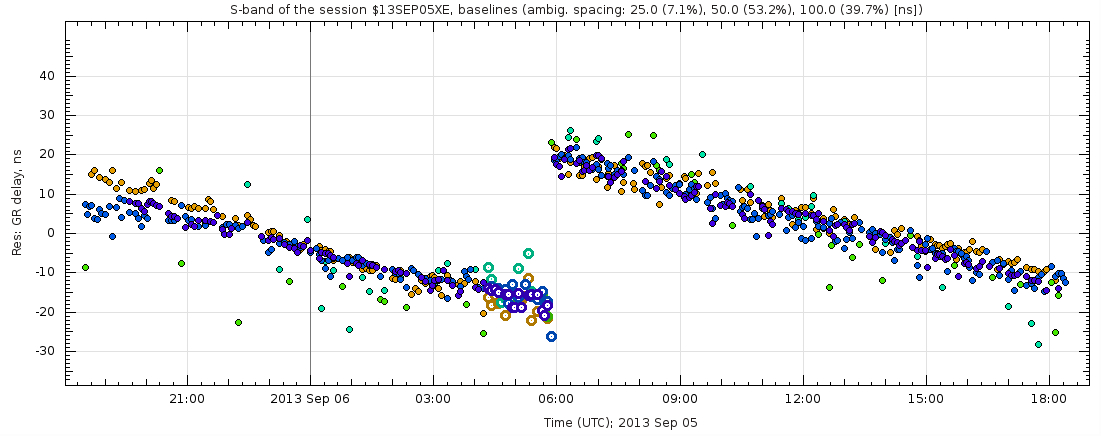
\includegraphics[width=.7\textwidth]{example-pass-04-2.jpg}
    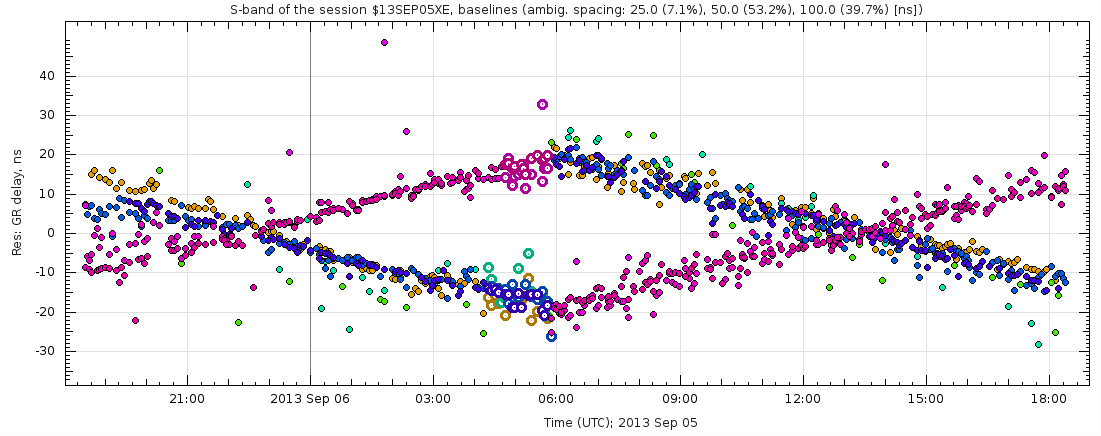
\includegraphics[width=.7\textwidth]{example-pass-04-3.jpg}
  \end{center}
  \caption{Session 13SEP05XE: group delay residuals. Processing a clock break.}
  \label{fig-ex-pass-04}
\end{figure}

The description of the clock break event
consists of the station name, the epoch of the break, and the magnitude
(for the first type of clock breaks) of the break. There are three options for processing a clock break. With
the first option, manual, the user specifies the parameters of the break
explicitly in a special window (see Fig.~\ref{fig-stnedit-cbe}). With
the second option, semiautomatic, the user provides to \nuSolve{} the
station name and the epoch of the break, and \nuSolve{} evaluates the
magnitude of the break. This option will be discussed in detail later.
With the last option, automatic, the software searches for a clock break
and evaluates parameters by itself. To invoke this procedure, press the
{\sl CBreak} button in the bottom of the Session Editor window. It
should work fine for this session (with proper {\it a~priori} files and
correctly resolved ambiguities), but the procedure for clock break
detection currently is in the embryonic stage, and there are cases where
it will not work.

\begin{figure}[htb!]
  \begin{center}
    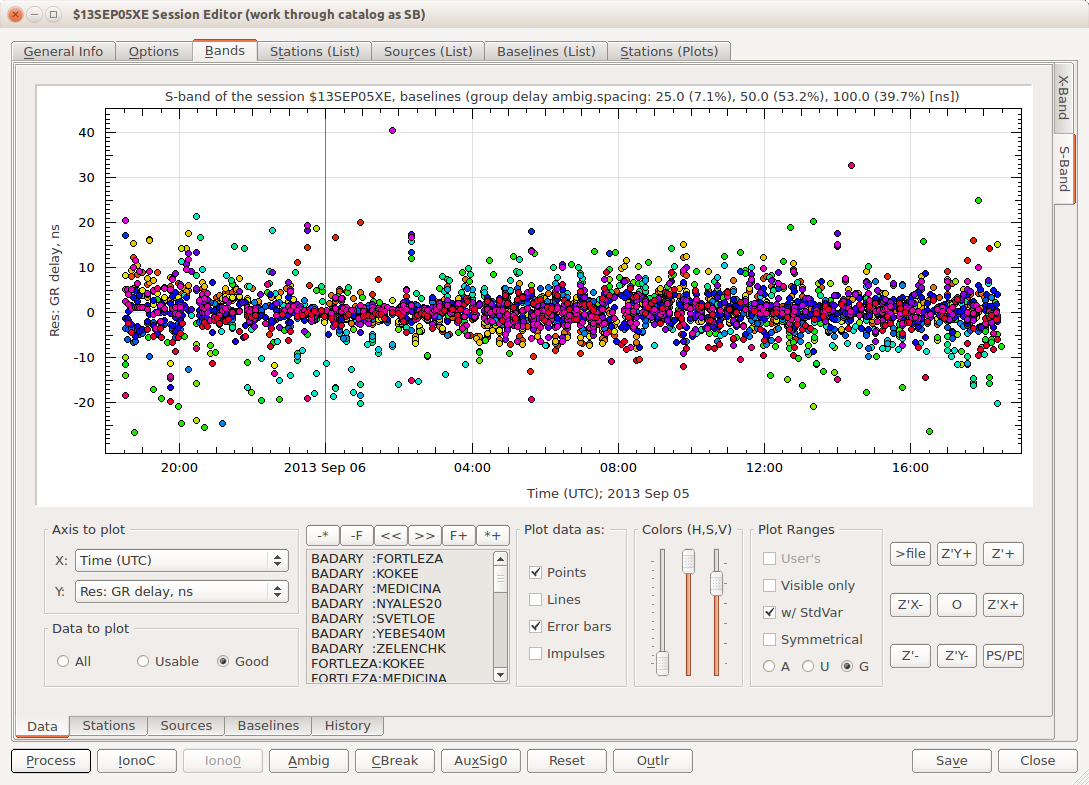
\includegraphics[width=1.0\textwidth]{example-pass-05.jpg}
  \end{center}
  \caption{Session 13SEP05XE: group delay residuals on the S-band.
           The clock break at SVETLOE is taken into account.}
  \label{fig-ex-pass-05}
\end{figure}


Here we will describe how to deal with clock breaks in semiautomatic
mode. If you already pressed the {\sl CBreak} button and the break
has vanished, just delete the clock break record. To do it, follow the
instructions:

\begin{itemize}
\item[--] if the option {\sl Estimate clock break parameters in common solution}
          is turned <<off>>, in the tab {\sl Bands} select sub-tab {\sl Stations}
          (at the bottom of the tab). Otherwise, select the tab {\sl Stations (List)};
\item[--] double click on the station SVETLOE -- a station parameter
          editor will appear;
\item[--] highlight the clock break entry in the {\sl List of Clock
          Break Events} and press the {\sl Delete} button;
\item[--] answer with the {\sl Yes} button on the prompt about
          deletion;
\item[--] close the window with the {\sl Ok} button;
\item[--] return back to the {\sl Data} sub-tab;
\item[--] press the {\sl Process} button to recalculate the
          residuals.
\end{itemize}


As a result, you should get the same distribution of residuals as before
in Fig.~\ref{fig-ex-pass-03}. To process a clock break in semiautomatic mode, we
need to highlight the rightmost points before the break in the few
baselines where the break has occurred. Here is a step-by-step
instruction of how to do it. First, press the {\sl -*} button above
the list of baselines of the plot to unselect all the data. Then, click
with mouse right button on the button {\sl F+} above the baseline
list and select from the menu the entry {\sl SVETLOE:}. The plotter
will select only those baselines in which SVETLOE is the first station.
Mark the points before the clock break by pressing the left mouse button
and drag the marking area to include the points (see
Fig.~\ref{fig-plot-canvas-seletion}). At the end, you should get a plot
such as the one shown in the top part of Fig.~\ref{fig-ex-pass-04}.



Unselect all baselines by pressing the {\sl -*} button, and click
mouse right button on the button {\sl F+} again. This time, choose
the entry {\sl :SVETLOE} to select the baselines in which SVETLOE is
the second station. Again, mark the rightmost points before the break.
You should get a plot such as the one shown in the middle part of
Fig.~\ref{fig-ex-pass-04}.

Left click on the button {\sl F+}, and choose station {\sl SVETLOE}.
All baselines with SVETLOE will be visible (see the bottom part of
Fig.~\ref{fig-ex-pass-04}).

Press the {\sl Ctrl+b} key combination. The software will use the
marked points to figure out the station at which the clock break
occurred and when it occurred. Also, the software will estimate the
magnitude of the clock break and adjust the residuals for its value.

Select all baselines using the button {\sl *+}, and press the {\sl
Process} button to refresh the residuals. At this stage you should
get a distribution such as the one shown in Fig.~\ref{fig-ex-pass-05}.

If necessary, recalculate the ambiguities (using the {\sl Ambig}
button), update the residuals (using the {\sl Process} button) and
re-estimate the magnitude of the clock break (using the {\sl Ctrl+b}
key combination).

\begin{figure}[htb!]
  \begin{center}
    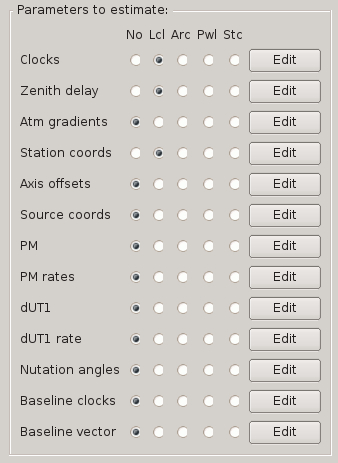
\includegraphics[width=0.3\textwidth]{example-estimation-02.jpg}
  \end{center}
  \caption{Estimated parameters}
  \label{fig-ex-est-02}
\end{figure}

Because the station and the epoch of the clock break is known, every
time a user presses the {\sl Ctrl+b} keys, \nuSolve{} will use these
pieces of information to calculate the magnitude of the break; no other
point selection is necessary. Also, sometimes it happens that several
stations have clock breaks or that a station has several clock breaks.
In this case you need to mark and then press the {\sl Ctrl+b} keys
to notify \nuSolve{} about each clock break. One by one, all known clock
breaks will be included in the estimation procedure.


You do not need to perform the procedure of selecting points as
described above. The software checks the marked points to figure out the
station name (it uses the most frequent name) and the epoch of the break
(it takes the latest epoch from the marked points). So, if you are sure,
it is enough to mark just two baselines with a clock break without any
operations of baseline selection and deselection.

Because we resolved the group delay ambiguities and fixed the clock
break at SVETLOE, we can extend our parameterization model and include
zenith delays and station positions as local parameters as shown in
Fig.~\ref{fig-ex-est-02}.


\begin{figure}[htb!]
  \begin{center}
    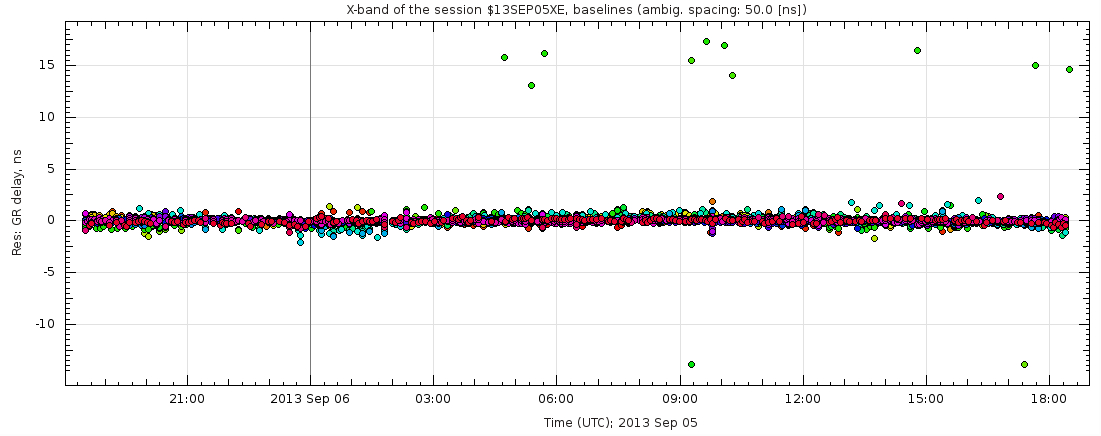
\includegraphics[width=.7\textwidth]{example-pass-06-1.jpg}
    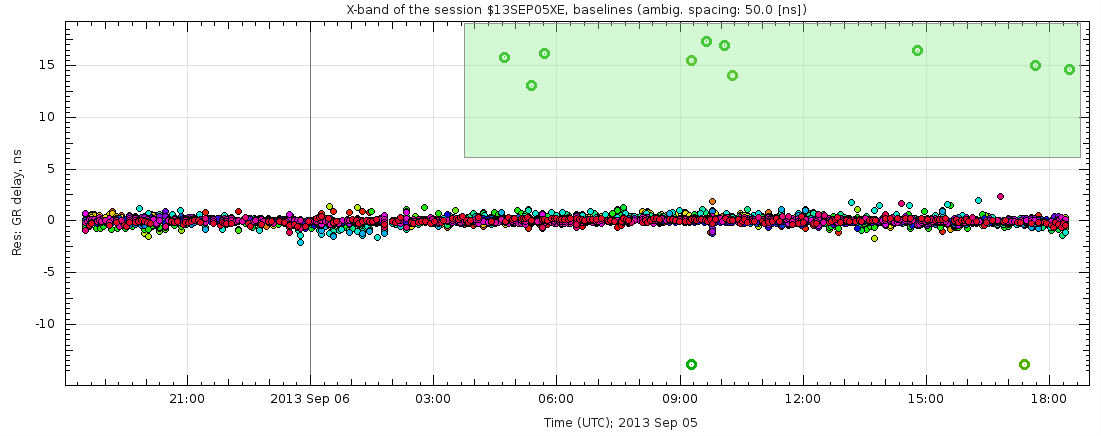
\includegraphics[width=.7\textwidth]{example-pass-06-2.jpg}
    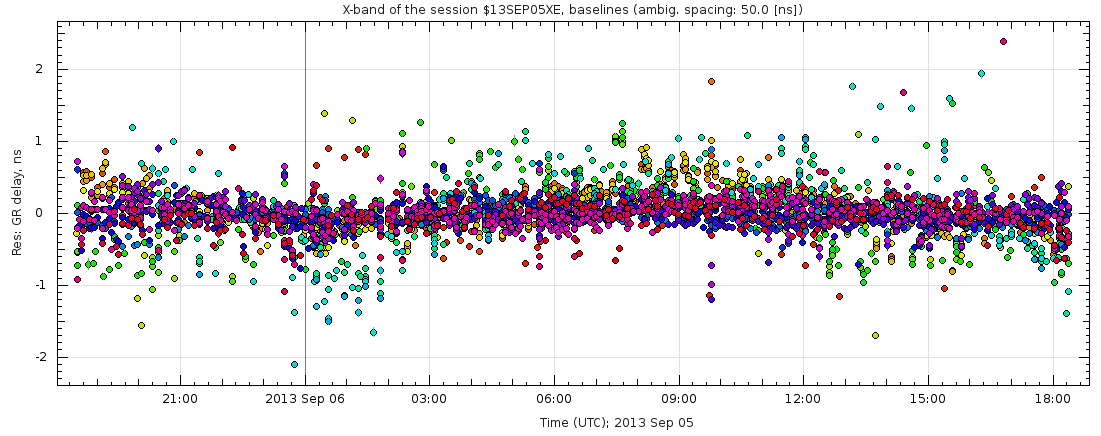
\includegraphics[width=.7\textwidth]{example-pass-06-3.jpg}
  \end{center}
  \caption{Session 13SEP05XE: group delay residuals. Removing large outliers.}
  \label{fig-ex-pass-06}
\end{figure}

\noindent
Select the X-band sub-tab and press the {\sl Process} button to
obtain a new solution. You should get a distribution of residuals
similar to the top plot of Fig.~\ref{fig-ex-pass-06}. As one can see,
there are several points that have residuals on the level of $13-15ns$.
These are examples of large outliers. Before continuing, we want to
remove them. Mark these points, as shown in the middle plot of the
figure, and press the {\sl Ctrl+x} key combination. Repeat the
solution to refresh the residuals. You should get a picture as shown in
the bottom plot of Fig.~\ref{fig-ex-pass-06}.

Check the residuals for every baseline, repeatedly clicking on the {\sl
``\textgreater\textgreater''} button above the baseline names of the
plot, to be sure that there are no any other effects that look like
clock breaks.

\begin{figure}[htb!]
  \begin{center}
    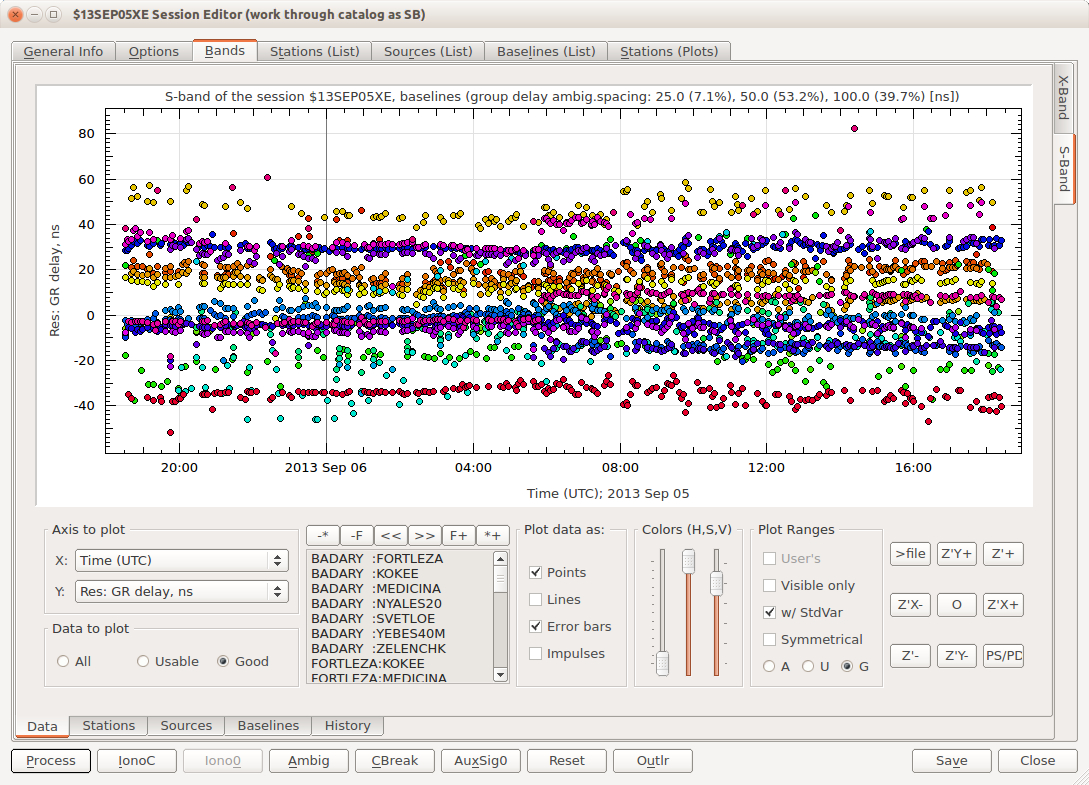
\includegraphics[width=1.0\textwidth]{example-pass-07.jpg}
  \end{center}
  \caption{Session 13SEP05XE: group delay residuals on the S-band.}
  \label{fig-ex-pass-07}
\end{figure}

When you done with X-band, switch to S-band. When a user estimates
parameters for a specified type of observable (single band delay, group
delay, etc.) and selected band, \nuSolve{} evaluates residuals for all
bands and observables with respect to the obtained parameters.
Therefore, when you switch to the S-band data, the residuals should look
completely different, see Fig.~\ref{fig-ex-pass-07}. The reason for this
is the influence of the ionosphere. We did not calculate the ionospheric
corrections yet; therefore the parameter estimations for the two
different frequency bands are different.

\begin{figure}[htb!]
  \begin{center}
    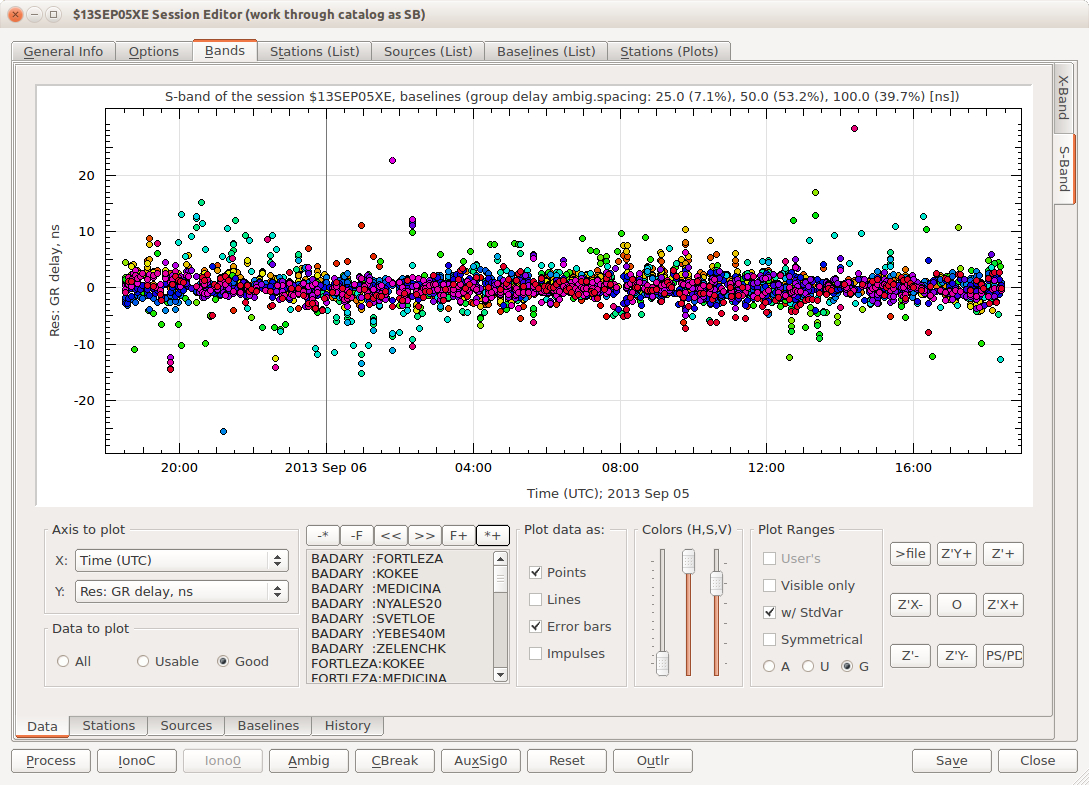
\includegraphics[width=1.0\textwidth]{example-pass-08.jpg}
  \end{center}
  \caption{Session 13SEP05XE: group delay residuals on the S-band.}
  \label{fig-ex-pass-08}
\end{figure}

Press the {\sl Process} button to recalculate the residuals for this
band. If necessary, repeat the procedure for ambiguity resolution.

Now we can set a ``standard'' number of polynomial coefficients for the
clock model. Go to the {\sl Stations (List)} tab and right click in the
column {\sl \#Clk.Terms} to increase the number of polynomial
coefficients to three for each station except the clock reference
station. To decrease the number, left click in the column. Usually, we
set the number of polynomial clock terms to three to be compatible with
CALC/SOLVE. However, sometimes a station's clock behavior can have
strongly expressed higher polynomials. In this case you can set up
higher polynomial orders. Also, you can set the standard polynomial
order during the early stages of data processing. There are no
restrictions --- just use common sense.

Again, recalculate the residuals and, if necessary, repeat the procedure
for ambiguity resolution. Check the residuals for every baseline (using
the {\sl ``\textgreater\textgreater''} and {\sl ``\textless\textless''}
buttons) for effects that look like clock breaks. At the end you should
get residuals as shown in Fig.~\ref{fig-ex-pass-08}.

Also, for S-band it frequently happens that for some baselines the
ambiguity spacings are less than the nominal $100ns$ value. For this
session they are: baseline MEDICINA:YEBES40M ($25ns$) and other baselines
with MEDICINA and baselines with FORTLEZA and ZELENCHK ($50ns$). We
strongly recommend inspecting the residuals at these baselines for
unresolved ambiguities and fixing them, if necessary, manually. To check
the ambiguity spacings of baselines, you can plot ambiguity spacings as
a function of time. Click on the combo box next to the {\sl Y} label
of the {\sl Axis to plot} group of the plot and choose {\sl Ambig
spacing, ns} to display the data. A double click on a point will open
a window with information about the corresponding observation.




%%%%%%%%%%%%%%%%%%%%%%%%%%%%%%%%%%%%%%%%%%%%%%%%%%%%%%%%%%%%%%%%%%%%%%%%%%%%
%%
%%
%%
%%%%%%%%%%%%%%%%%%%%%%%%%%%%%%%%%%%%%%%%%%%%%%%%%%%%%%%%%%%%%%%%%%%%%%%%%%%%
\subsection{Ionosphere correction}
To evaluate the ionosphere corrections, press the {\sl IonoC} button
at the bottom of the Session Editor window and recalculate the
residuals. After this procedure the residuals for X-band will look as
shown in Fig.~\ref{fig-ex-pass-09}.

\begin{figure}[htb!]
  \begin{center}
    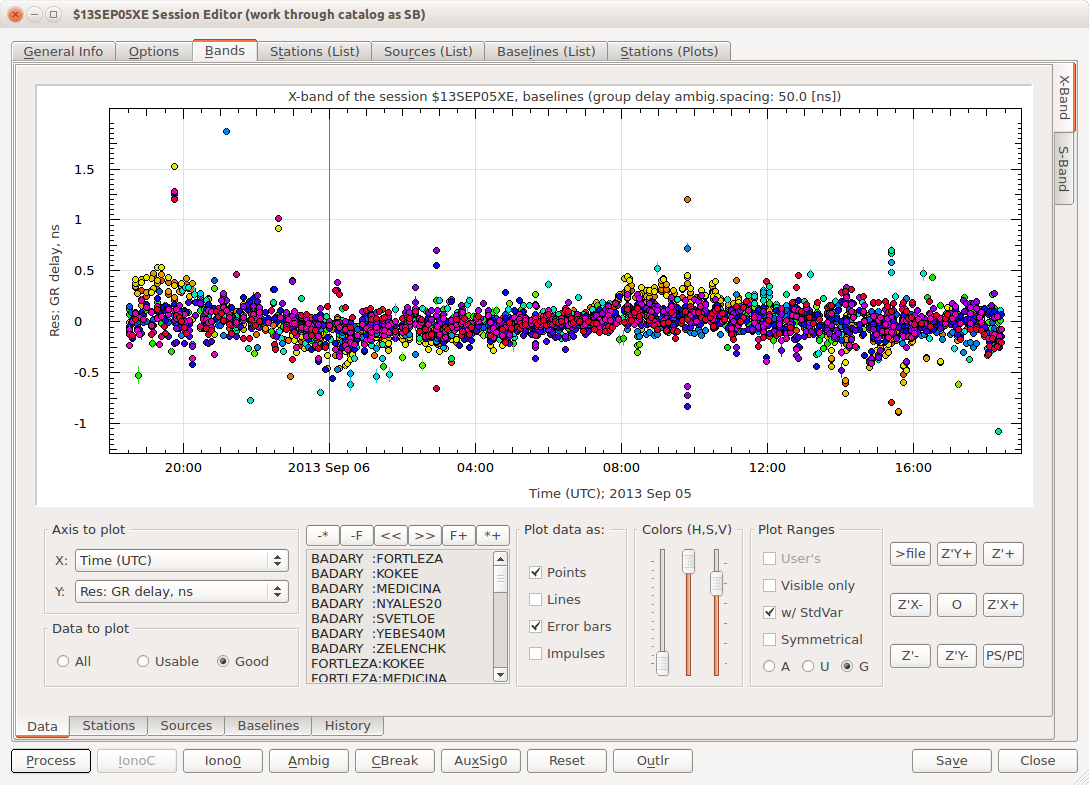
\includegraphics[width=1.0\textwidth]{example-pass-09.jpg}
  \end{center}
  \caption{Session 13SEP05XE: group delay residuals.}
  \label{fig-ex-pass-09}
\end{figure}

At this stage, when the ionospheric corrections are added to the model,
the residuals for X-band and S-band look similar; the difference is only
in the standard deviations of observations. In fact, for both cases we
have an <<ionosphere free combination>> of dual frequency observations.

It is worth noting that if there are some unresolved ambiguities or
clock breaks, they will affect the ionosphere corrections and, as a
result, the residuals of both bands at this stage. Check the baselines
one by one. If you notice one of these effects, remove the ionospheric
corrections by pressing the {\sl Iono0} button, find the band where
the effect appears, and fix it. Then, repeat the procedure of
calculating the ionosphere corrections.

Once the ionospheric corrections have been calculated, all other
solutions are made using the observations at X-band.



%%%%%%%%%%%%%%%%%%%%%%%%%%%%%%%%%%%%%%%%%%%%%%%%%%%%%%%%%%%%%%%%%%%%%%%%%%%%
%%
%%
%%
%%%%%%%%%%%%%%%%%%%%%%%%%%%%%%%%%%%%%%%%%%%%%%%%%%%%%%%%%%%%%%%%%%%%%%%%%%%%
\subsection{Obtaining a full solution}
Now we can set up the <<standard>> set of parameters. Usually, we
estimate clocks and zenith parameters as piecewise-continuous functions, and
we treat the station positions, rate of Earth rotation, angles of
nutation, and baseline clock offsets as local parameters, see
Fig.~\ref{fig-ex-est-03}.

\begin{figure}[htb!]
  \begin{center}
    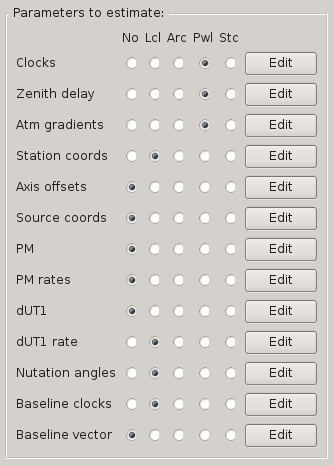
\includegraphics[width=0.3\textwidth]{example-estimation-03.jpg}
  \end{center}
  \caption{Estimated parameters.}
  \label{fig-ex-est-03}
\end{figure}

To configure a piecewise-continuous (PWL) function, press the {\sl Edit}
button (see the figure). For the PWL mode, there are two values --- the
interval of a piece and the magnitude of the constraints that have to be
applied to the variations of the parameter. By default, the interval for
the clocks and for the zenith delays is one hour. The constraints for
clocks are 72~ps/hr and for zenith delays are 1.1992~cm/hr. These values
conform to the default values of interactive SOLVE, 2.00~D-14 and
40.00~ps/hr, respectively. For the atmospheric gradients, the default
value for the interval is 28.8~hr, which is supposed to be greater than
the length of a session. In this case, \nuSolve{}, as well as
interactive SOLVE, will adjust the PWL interval to the length of the
session. The default constraints for the gradients are loose; currently,
they are $10^9$~m/hr.

If you turned on the baseline clock offsets, you need to select the
baselines for which the clock offsets will be estimated. In contrast to
the flags for other estimated parameters, the ``estimate clock offset''
flag for each baseline is turned off by default. To turn these flags on,
go to the tab {\sl Baselines (List)} and turn on the proper flag as
described in the subsection \ref{subsect-sessedit-baselines}. Not all baselines
require estimation of a clock offset. Use this parameter only for
baselines that reveal significant clock offsets.

\begin{figure}[htb!]
  \begin{center}
    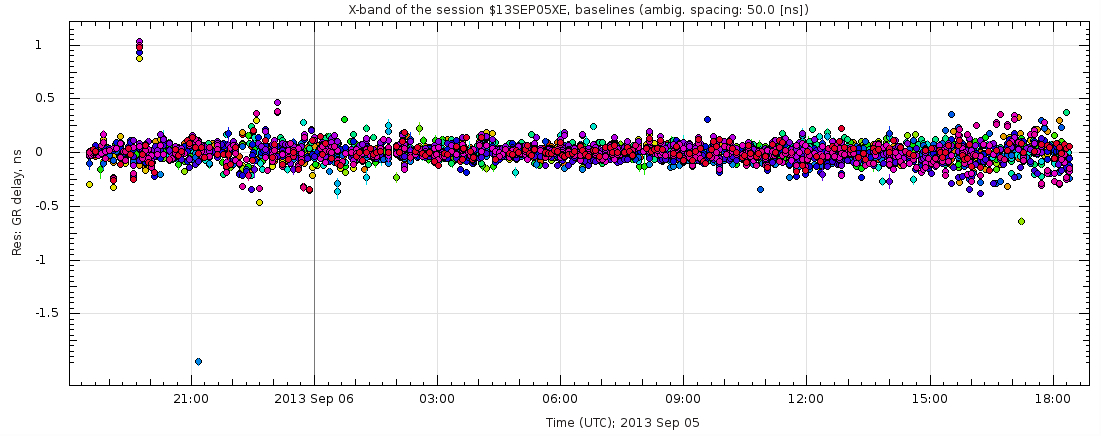
\includegraphics[width=1.0\textwidth]{example-pass-10.jpg}
  \end{center}
  \caption{Session 13SEP05XE: group delay residuals.}
  \label{fig-ex-pass-10}
\end{figure}

Press the {\sl Process} button to estimate parameters. Check for
large outliers. Fig.~\ref{fig-ex-pass-10} displays the residuals. As one
can see, there are a few observations that have large residuals. We
exclude them from the solution. It is (relatively) safe because later we
will add into the analysis all observations that were previously
excluded or were never included at all, if they have residuals less than
three sigmas. On the other hand, manually exclude observations that are
really large outliers (i.e., that have residuals of, perhaps, eight
sigmas and higher, see plots of {\sl Normalized residuals}).

Also, it is worthwhile to check the obtained solutions. The estimations
of the local parameters are printed in the log output. The estimations
of time varying clock and troposphere parameters are plotted on the plot
of the {\sl Stations (Plots)} tab. Select {\sl Est.Clocks, ps}
as the {\sl Y} axis to check the estimations of clocks, {\sl
Est.Zenith, ps} to check the wet zenith delays, and {\sl
Est.AtmGrd:N, cm} and {\sl Est.AtmGrd:E, cm} to check the
tropospheric gradients in the north and the east directions.


%%%%%%%%%%%%%%%%%%%%%%%%%%%%%%%%%%%%%%%%%%%%%%%%%%%%%%%%%%%%%%%%%%%%%%%%%%%%
%%
%%
%%
%%%%%%%%%%%%%%%%%%%%%%%%%%%%%%%%%%%%%%%%%%%%%%%%%%%%%%%%%%%%%%%%%%%%%%%%%%%%
\subsection{Reweighting of observations}
To make a reduced $\chi^2$ close to unity, \nuSolve{} (as well as interactive
SOLVE) calculates additional sigmas that will be added to the standard
deviations of the observations to compute the weights of the
observations. The algorithm of calculation of the additional sigmas is
described in \cite{Petrov1998}.

Since these calculations are made during data processing,
to turn on the procedure of reweighting, check the {\sl Evaluate
weight correction} box of the {\sl Reweighting} group at the {\sl
Options} tab. When you press the {\sl Process} button next time,
the weight corrections will be evaluated. To put them into effect, a
user needs to repeat data analysis. This is a converging process.
Usually you need to make three to four iterations to obtain the proper
additional sigmas.

The weight corrections are calculated in two modes: independently for
each baseline and for the whole band (see the {\sl Reweighting mode}
radio button in {\sl Options}). Depending on the mode, the user can
check the evaluated weight corrections either in the column {\sl
Sigma\_0} at the tab {\sl Baselines (List)} or in the column
{\bf $\sigma_0$} of the group {\sl Bands} at the tab {\sl General
Info}.

There are two shortcut keys, {\sl Alt-2} and {\sl Alt-3}.
Pressing these keys are equivalent to clicking the {\sl Process}
button two and three times respectively.



%%%%%%%%%%%%%%%%%%%%%%%%%%%%%%%%%%%%%%%%%%%%%%%%%%%%%%%%%%%%%%%%%%%%%%%%%%%%
%%
%%
%%
%%%%%%%%%%%%%%%%%%%%%%%%%%%%%%%%%%%%%%%%%%%%%%%%%%%%%%%%%%%%%%%%%%%%%%%%%%%%
\subsection{Outlier processing}
When the procedure of reweighting is completed, we can remove outliers.
By ``outlier'' we mean an observation with an absolute normalized
residual greater than a user-specified threshold. The residuals are
normalized either by a dispersion, as it is described in \cite{Petrov1997},
or by WRMS. The normalization with the dispersion
is done if the checkbox {\sl Use SOLVE compatible mode} is <<on>>,
otherwise, the WRMS are used.

By default, the
threshold is set to three (the normalized residuals are unitless; with
some assumptions, this corresponds to $3\sigma$ for non-normalized
residuals). The procedure is iterative. \nuSolve{} searches for the
observation with the largest normalized residual, deselects it from the
data analysis and obtains a new solution. Then it repeats the procedure.
The user can change the maximum number of iterations. By default, this
value is equal to 40 (see the {\sl Options} tab).

To initiate the procedure for outlier processing, press the {\sl
Outlr} button at the bottom of the Session Editor window. \nuSolve{}
will start to deselect outliers and recalculate the solution. It can
take some time.

By default, when the software recalculates the solution after the
elimination of an outlier, the reweighting coefficients are not
calculated. After the iterations have finished, make several solutions
to refresh the reweighting corrections and keep reduced $\chi^2$ close to unity.

There is also a shortcut, {\sl Alt-4}, that is equivalent to
clicking on the {\sl Outlr} button and then pressing the {\sl
Alt-3} key combination.

When you get to the stage where there are no outliers to remove, change
the action of outlier processing from {\sl Elimination} to {\sl
Restoration} at the {\sl Options} tab, in the {\sl Outliers
Action} group of radio buttons. Repeat the outlier processing. With
the restoration action, \nuSolve{} includes in the data analysis all
observations that have normalized residuals less than the threshold.

Repeat the elimination and restoration actions. At the end, there should
not be any observations that can be either eliminated or restored.

At this stage, check the baseline clock offsets again. When the
reweighting is done, the estimations will not be so optimistic, and the
number of significant clock offsets will decrease. If necessary, repeat
the procedure of outlier processing.



%%%%%%%%%%%%%%%%%%%%%%%%%%%%%%%%%%%%%%%%%%%%%%%%%%%%%%%%%%%%%%%%%%%%%%%%%%%%
%%
%%
%%
%%%%%%%%%%%%%%%%%%%%%%%%%%%%%%%%%%%%%%%%%%%%%%%%%%%%%%%%%%%%%%%%%%%%%%%%%%%%
\subsection{Saving the results}
To save the edited session, press the {\sl Save} button at the
bottom of the Session Editor window. The session will be saved in the
corresponding format. Also, a file in the interactive SOLVE {\sl
spoolfile} format will be generated.





%%%%%%%%%%%%%%%%%%%%%%%%%%%%%%%%%%%%%%%%%%%%%%%%%%%%%%%%%%%%%%%%%%%%%%%%%%%%
%%
%%
%%
%%%%%%%%%%%%%%%%%%%%%%%%%%%%%%%%%%%%%%%%%%%%%%%%%%%%%%%%%%%%%%%%%%%%%%%%%%%%
\section{Using a source structure model}
\label{section-using-gui-ssm}

The recent VGOS observations showed that the effect of source structures becomes
detectable in the broadband group delays. To take into account this effect
a simple multi point source structure model is implemented in \nuSolve{}, see
\cite{Bolotin2019} for details.

To turn on using the model, a user should check on the checkbox {\sl Apply source
structure model} of the "General configure editor" or "Options" tab of the
"Session editor". A source for which the model should be applied have to have
the attribute "Apply the multi point source structure model" set to <<on>>.
It can be done with the source attribute editor (see
\emph{\ref{subsubsect-sessedit-source-attr-edit} Source Attributes Editor}) or
clicking at the corresponding row of the column {\sl UseSSM} of the sources list,
\emph{\ref{subsect-sessedit-sources-list} Tab <<Sources (List)>>}).

Components of the model should have non-zero position and ratio of brightness.
To edit the parameters of a component manually, use the source structure model
component Editor (see Fig.~\ref{fig-srcedit-ssm}).

Another option to provide parameters of the model is to set up a file with a
list of sources and their source structure model components. Using of such file
is configuring in the tab {\sl External a priori and models}
(see the subsection \emph{\ref{sect-config-models} Applying different models
and using external a priori information}). If the file is exist and the checkbox
{\sl Source structure model} is on, then the file will be read after loading a
session.

The file has the following format. Any string that starts with a char <<\$>>,
<<\#>>, <<*>> or <</>> is considered as a comment line. Each line consist of
a token (case insensitive) and its value pairs:
\begin{verbatim}
Token:Value
\end{verbatim}
\noindent
A line that has a token-value pair {\tt Src:<SourceName>} specifies a source
and a first component of the model. A pair {\tt SSM\_T:MP} determines that the type
of a source structure model is the multi point model. Tokens {\tt x} and {\tt y} provide
relative coordinates of the component. A token {\tt K} sets the brightness ratio
and a token {\tt B} -- a difference of spectral indices. Tokens
{\tt ER }, {\tt EK } and {\tt EB } specify which parameters should be estimated:
position of a component, ratio $k$ or difference of spectral indices $\beta$ correspondingly.
A token {\tt T } specifies an epoch since that the model is valid. The tokens
{\tt x }, {\tt y } and {\tt k } are mandatory if the model type is {\tt MP }.
If other parameters are not specified, they will be zero ($\beta$), <<no>> ({\tt ER },
{\tt EK } and {\tt EB }) and some very early epoch for {\tt T }.
If a source structure model has more than one secondary component, the token
{\tt Src: } should be omitted.

For example, the records
\begin{verbatim}
Src:0016+731 SSM_T:MP i:1 x:-0.5970 y: 0.0894 K:0.1850 B: 4.2510  ER:No EK:No EB:No
                      i:2 x:-0.7031 y: 0.7141 K:0.0852 B: 0.8741  ER:No EK:No EB:No

Src:0016+731 SSM_T:MP i:1 x:-0.5231 y: 0.0627 K:0.5320 B:-0.4592  ER:No EK:No EB:No T:2018/01/01
\end{verbatim}
\noindent
specifies that if a first epoch of observations is before January 1, 2018 then the
model with two secondary components will be used, otherwise a model with one secondary
component will be applied.

If the brightness ratio, K, is not fall into realistic interval, ]0..1[, or
both coordinates, x and y, are zeros, then the model will be turned off. It can be useful
when you have a time tag <<T:>> to specify since when the model should not be
applied.

Number of spaces between tokens can be arbitrary. The tokens {\verb i:1 }, {\verb i:2 }, etc.
are not used, they are added mostly for user convenience.

An example of such file is distributed along with the software, see {\tt data/glo.ssm}
file. Starting with the distribution version 0.7.1, this file contains results of estimation
of the parameters of the source structure model from available at this time VGOS
sessions. Currently, the estimations are available for several radio sources:
0016+731, 0059+581, 0119+115, 0552+398 and 3C371. In future, this list, perhaps, will
be extended.


To estimate parameters of a model component, a user should set to "Lcl" the corresponding
checkbox, {\sl Source structure model} of the widget group {\sl Parameters to estimate}
of the tab {\sl Operation}. In contrast to other estimated parameters, the components of
the model are accumulating the estimated values. It means that after each iteration
the obtained estimations are added to their a priori values. It is done to find out
how meaningful the estimations are. The model is highly non linear, it is strongly
depend on initial (a priori) values. If a model is real, than with each iteration
the estimations will go smaller and smaller, the positions of a component will be
in a circle of tens mas, the $k$ ratio will be bigger than $0$ and less than $1$.
Everything else should be considered as misfitting.












%%%%%%%%%%%%%%%%%%%%%%%%%%%%%%%%%%%%%%%%%%%%%%%%%%%%%%%%%%%%%%%%%%%%%%%%%%%%
%
%
%
%
\chapter{Scripting support}
\label{chapter-scripting}


%%%%%%%%%%%%%%%%%%%%%%%%%%%%%%%%%%%%%%%%%%%%%%%%%%%%%%%%%%%%%%%%%%%%%%%%%%%%
%%
%%
%%
%%%%%%%%%%%%%%%%%%%%%%%%%%%%%%%%%%%%%%%%%%%%%%%%%%%%%%%%%%%%%%%%%%%%%%%%%%%%
\section{ECMAScript in \nuSolve{}}
\label{section-scripting-intro}
The scripting abilities in \nuSolve{} are in development stage. The
software uses the script engine that is provided by Qt library (QtScript
module). This is a realization of ECMAScript, a standardized version
of JavaScript -- simple, powerful and flexible object oriented scripting
language. Documentation and user guides are available on the Net,
one of the link is:
\begin{verbatim}
      https://developer.mozilla.org/en-US/docs/Web/JavaScript/Guide
\end{verbatim}

To realize scripting in \nuSolve{} we made some classes and objects
accessible to the script engine. Since this feature of the software is
in active development phase, the list of available for script objects
will be extended in the future.

To invoke a script in \nuSolve{} a user should provide a file name of
the script with <<-t>> option, e.g.:
\begin{verbatim}
    > nuSolve -t pia4INT.js
\end{verbatim}
\noindent
Here the file {\tt pia4INT.js} is a script that executes all post import
actions for INT type of a VLBI session, see~\ref{subsect-config-pia}.
This file is a part of nusolve distribution and can be found in a
directory {\sl scripts} of the distribution.

If a file cannot be found in the current directory, \nuSolve{} will
search a file with the provided name in the system wide directory
(can be altered during execution of {\tt configure} script, see Chapter
\emph{\ref{chapter-installation} Installation}). This feature allows
a user to skip path to the scripts that are provided by the distribution.

When a user invokes \nuSolve{} to execute a script, the software uses the
standard or altered configuration. However, it does not save changes to
the configuration that were made in a script. So it is safe to modify
options, models, parameters, etc.

In the following sections we discuss the internal objects that are accessible
to the script engine.




%%%%%%%%%%%%%%%%%%%%%%%%%%%%%%%%%%%%%%%%%%%%%%%%%%%%%%%%%%%%%%%%%%%%%%%%%%%%
%%
%%
%%
%%%%%%%%%%%%%%%%%%%%%%%%%%%%%%%%%%%%%%%%%%%%%%%%%%%%%%%%%%%%%%%%%%%%%%%%%%%%
\section{Software set up in scripts}
\label{section-scripting-setup}
Changing the software setup (see Chapter~\ref{chapter-config}) in a script is done
through an object {\sl setup}.
The properties of the object are shown on the table
Tab.~\ref{tab-scr-setup-properties}.

The properties have read/write access, so user can change them. After end of script
execution, the modified properties will not be saved (in contrast to the interactive
mode). An example of using the object {\sl setup}:
{\small\begin{verbatim}
    setup.path2SpoolFileOutput = 'spoolfiles-tests';
    setup.have2KeepSpoolFileReports = true;
    print('Path to spool files: ' + setup.path2SpoolFileOutput);
    print('Have to keep spool files: ' + setup.have2KeepSpoolFileReports);
\end{verbatim}}
\noindent
will generate the following output:
{\small\begin{verbatim}
Path to spool files: spoolfiles-tests
Have to keep spool files: true
\end{verbatim}}



\begin{table}[htb]
\centering
\footnotesize
%\scriptsize
%\begin{tabular}{l p{0.75\textwidth}}
\begin{tabular}{lllp{0.40\textwidth}}
\hline
Type & Property & Access & Meaning\\
\hline
  {\bf String}   & path2Home                 & Read/Write & a path to software home directory\\
  {\bf String}   & path2CatNuInterfaceExec   & Read/Write & a path to the Catalog <--> nuSolve Interface \\
  {\bf String}   & path2DbhFiles             & Read/Write & a path to VLBI sessions in DBH format \\
  {\bf String}   & path2VgosDbFiles          & Read/Write & a path to VLBI sessions in vgosDb format\\
  {\bf String}   & path2VgosDaFiles          & Read/Write & a path to VLBI sessions in vgosDa format\\
  {\bf String}   & path2APrioriFiles         & Read/Write & a path to search for a priori files\\
  {\bf String}   & path2MasterFiles          & Read/Write & a path to read master files\\
  {\bf String}   & path2SpoolFileOutput      & Read/Write & a path to write a spool file\\
  {\bf String}   & path2NotUsedObsFileOutput & Read/Write & a path where to put observations info\\
  {\bf String}   & path2ReportOutput         & Read/Write & a path where to save reports in the spool file format\\
  {\bf String}   & path2NgsOutput            & Read/Write & a path where to store NGS files\\
  {\bf String}   & path2PlotterOutput        & Read/Write & a path to plotter's output\\
  {\bf boolean}  & have2UpdateCatalog        & Read/Write & if {\sl true} the software will use the catalog\\
  {\bf boolean}  & have2MaskSessionCode      & Read/Write & save a session with alternative database name\\
  {\bf boolean}  & have2KeepSpoolFileReports & Read/Write & copy a spool file into {\sl path2ReportOutput} directory\\
  {\bf boolean}  & have2LoadImmatureSession  & Read/Write & load a session that does not have all data\\
  {\bf boolean}  & have2AutoloadAllBands     & Read/Write & automatically load all available bands\\
  {\bf String}   & pwd                       & Read       & an absolute path of the current directory\\
%  String  path2AuxLogs
%  boolean have2SavePerSessionLog
\hline
\end{tabular}
\caption{Execution control properties of {\sl setup} object.}
\label{tab-scr-setup-properties}
\end{table}

%
%
%
%
%%%%%%%%%%%%%%%%%%%%%%%%%%%%%%%%%%%%%%%%%%%%%%%%%%%%%%%%%%%%%%%%%%%%%%%%%%%%
%%
%%
%%
%%%%%%%%%%%%%%%%%%%%%%%%%%%%%%%%%%%%%%%%%%%%%%%%%%%%%%%%%%%%%%%%%%%%%%%%%%%%
\section{Solution configuration in scripts}
\label{section-scripting-config}
To modify the configuration of a solution an object {\sl config} is available
in a script. The properties of the object are shown on the tables
Tab.~\ref{tab-scr-config-properties-1} -- \ref{tab-scr-config-properties-5}.
All properties have read/write access, so user can inquire or modify them.
For example, the commands in a script
{\small\begin{verbatim}
    config.qualityCodeThreshold = 4;
    print('QC threshold = ' + config.qualityCodeThreshold);
\end{verbatim}}
\noindent
will generate the following output:
{\small\begin{verbatim}
    QC threshold = 4
\end{verbatim}}

The first group of properties controls how a solution will be obtained.
They are shown on Tab~\ref{tab-scr-config-properties-1} and correspond to
the general options of software configuration (see subsection~\ref{sect-config-general}
for details).


\begin{table}[htb]
\centering
\footnotesize
%\scriptsize
%\begin{tabular}{l p{0.75\textwidth}}
\begin{tabular}{lllp{0.40\textwidth}}
\hline
Type & Property & Access & Meaning\\
\hline
  {\bf int} & qualityCodeThreshold & Read/Write & Quality Code threshold\\
  {\bf int} & goodQualityCodeAtStartup & Read/Write & initial Quality Code threshold for non-processed yet session\\
  {\bf boolean} & useGoodQualityCodeAtStartup & Read/Write & for new session initially use observations with Quality Code of {\sl goodQualityCodeAtStartup} or higher\\
  {\bf CFG.VlbiDelayType} & useDelayType & Read/Write & type of delay to use\\
  {\bf CFG.VlbiRateType} & useRateType & Read/Write & type of rate to use\\
  {\bf int} & activeBandIdx & Read/Write & index of the band to process\\
  {\bf boolean} & isSolveCompatible & Read/Write & run in interactive SOLVE compatible mode\\
  {\bf boolean} & useDynamicClockBreaks & Read/Write & estimate clock break parameters in a common solution\\
  {\bf boolean} & useSolveObsSuppresionFlags & Read/Write & use SOLVE observation elimination flag\\
  {\bf CFG.EstimatorPwlMode} & pwlMode & Read/Write & mode for piece-wise continuous function for parameters estimated as {\sl PWL}\\
  {\bf boolean} & doDownWeight & Read/Write & downweight delays\\
  {\bf boolean} & have2outputCovarMatrix & Read/Write & controls output of a covariance matrix in a spool file\\
\hline
\end{tabular}
\caption{Execution control properties of {\sl config} object.}
\label{tab-scr-config-properties-1}
\end{table}

The first column of the tables displays type of a property. ECMAScript has
one primitive type for integers and doubles, <<Number>>. In the table instead
of type {\bf Number} the two C++ types are shown ({\bf int} or {\bf double})
to make a user easier to figure out what values are expected by the software.
Another set of types are provided by the metaobject <<CFG>> (like
{\bf CFG.VlbiDelayType} on the Tab.~\ref{tab-scr-config-properties-1}), these types
will be discussed later.


\begin{table}[htb]
\centering
\footnotesize
%\scriptsize
\begin{tabular}{lllp{0.35\textwidth}}
\hline
Type & Property & Access & Meaning\\
\hline
  {\bf CFG.OutliersProcessingMode} & opMode & Read/Write & outlier processing mode, band-wide or for each baseline\\
  {\bf CFG.OutliersProcessingAction} & opAction & Read/Write & outlier processing action: remove an outlier from a solution or include it back\\
  {\bf double} & opThreshold & Read/Write & threshold for residuals to specify an outlier\\
  {\bf int} & opIterationsLimit & Read/Write & limit for a number of iterations\\
  {\bf boolean} & opHave2SuppressWeightCorrection & Read/Write & need to turn off weight corrections while running iterations\\
  {\bf boolean} & opHave2NormalizeResiduals & Read/Write & use normalized residuals to determine outliers\\
  {\bf boolean} & opIsSolveCompatible & Read/Write & evaluate the normalized residuals in SOLVE compatible mode\\
\hline
\end{tabular}
\caption{Outlier processing properties of config object.}
\label{tab-scr-config-properties-2}
\end{table}


The Tab.~\ref{tab-scr-config-properties-2} and Tab.~\ref{tab-scr-config-properties-3} shows properties that affects processing
of outliers and weight correction (as it described in the subsection~\ref{sect-config-runtime}).

\begin{table}[htb]
\centering
\footnotesize
%\scriptsize
\begin{tabular}{lllp{0.40\textwidth}}
\hline
Type & Property & Access & Meaning\\
\hline
  {\bf boolean} & doWeightCorrection & Read/Write & switches the evaluation of weight corrections\\
  {\bf CFG.WeightCorrectionMode} & wcMode & Read/Write & weight correction mode, band-wide or for each baseline\\
  {\bf boolean} & useExternalWeights & Read/Write & use an external file with precalculated weights\\
  {\bf String} & extWeightsFileName & Read/Write & a name of the external file\\
\hline
\end{tabular}
\caption{Weight correction properties of config object.}
\label{tab-scr-config-properties-3}
\end{table}

Manipulations with external a priori data (discussed in subsection~\ref{sect-config-models}) are
displayed on Tab.~\ref{tab-scr-config-properties-4}.

\begin{table}[htb]
\centering
\footnotesize
%\scriptsize
\begin{tabular}{lllp{0.45\textwidth}}
\hline
Type & Property & Access & Meaning\\
\hline
  {\bf boolean} & useExtAPrioriSitesPositions & Read/Write & use external site positions\\
  {\bf boolean} & useExtAPrioriSitesVelocities & Read/Write & use external site velocities\\
  {\bf boolean} & useExtAPrioriSourcesPositions & Read/Write & use external source positions\\
  {\bf boolean} & useExtAPrioriErp & Read/Write & use external ERP\\
  {\bf boolean} & useExtAPrioriAxisOffsets & Read/Write & use external axis offsets\\
  {\bf boolean} & useExtAPrioriHiFyErp & Read/Write & use external model for subdiurnal ERP variations\\
  {\bf boolean} & useExtAPrioriMeanGradients & Read/Write & use external mean atmospheric gradients\\
  {\bf boolean} & useExtAPrioriSsm & Read/Write & use external file with source structure models\\
  {\bf String} & extAPrioriSitesPositionsFileName & Read/Write & a file name for site positions\\
  {\bf String} & extAPrioriSitesVelocitiesFileName & Read/Write & a file name for site velocities\\
  {\bf String} & extAPrioriSourcesPositionsFileName & Read/Write & a file name for source positions\\
  {\bf String} & extAPrioriErpFileName & Read/Write & a file name for ERP\\
  {\bf String} & extAPrioriAxisOffsetsFileName & Read/Write & a file name for axis offsets\\
  {\bf String} & extAPrioriHiFyErpFileName & Read/Write & a file name for subdiurnal ERP variations\\
  {\bf String} & extAPrioriMeanGradientsFileName & Read/Write & a file name for mean atmospheric gradients\\
  {\bf String} & extAPrioriSsmFileName & Read/Write & a file name for external source structure model\\
  {\bf String} & eccentricitiesFileName & Read/Write & a file name for eccentricities\\
\hline
\end{tabular}
\caption{Use of external a priori properties of config object.}
\label{tab-scr-config-properties-4}
\end{table}

\begin{table}[htb]
\centering
\footnotesize
%\scriptsize
\begin{tabular}{lllp{0.45\textwidth}}
\hline
Type & Property & Access & Meaning\\
\hline
  {\bf boolean} & have2ApplyPxContrib & Read/Write & apply contributions for the polar motion, X-component\\
  {\bf boolean} & have2ApplyPyContrib & Read/Write & apply contributions for the polar motion, Y-component\\
  {\bf boolean} & have2ApplyEarthTideContrib & Read/Write & apply contributions for solid Earth tides\\
  {\bf boolean} & have2ApplyOceanTideContrib & Read/Write & apply contributions for ocean tides loading\\
  {\bf boolean} & have2ApplyPoleTideContrib & Read/Write & apply contributions for pole tide deformations\\
  {\bf boolean} & have2ApplyUt1OceanTideHFContrib & Read/Write & apply contributions for subdiurnal UT1 variations\\
  {\bf boolean} & have2ApplyPxyOceanTideHFContrib & Read/Write & apply contributions for subdiurnal polar motion\\
  {\bf boolean} & have2ApplyNutationHFContrib & Read/Write & apply contributions for libration in ERP (CALC 10)\\
  {\bf boolean} & have2ApplyUt1LibrationContrib & Read/Write & apply contributions for libration in UT1 (CALC 11)\\
  {\bf boolean} & have2ApplyPxyLibrationContrib & Read/Write & apply contributions for libration in polar motion (CALC 11)\\
  {\bf boolean} & have2ApplyOceanPoleTideContrib & Read/Write & apply contributions for ocean pole tide loading\\
  {\bf boolean} & have2ApplyFeedCorrContrib & Read/Write & apply contributions for feed horn rotation\\
  {\bf boolean} & have2ApplyTiltRemvrContrib & Read/Write & apply contributions for axis tilt remover\\
  {\bf boolean} & have2ApplySsm & Read/Write & turn on/off using the source structure model\\
  {\bf boolean} & have2ApplyAxisOffsetContrib & Read/Write & apply contributions for axis offsets\\
  {\bf boolean} & have2ApplyNdryContrib & Read/Write & apply contributions for refraction, hydrostatic atmosphere\\
  {\bf boolean} & have2ApplyNwetContrib & Read/Write & apply contributions for refraction, wet atmosphere\\
  {\bf boolean} & have2ApplyOldOceanTideContrib & Read/Write & apply contributions for old model of ocean tides\\
  {\bf boolean} & have2ApplyOldPoleTideContrib & Read/Write & apply contributions for old model of ocean pole tides\\
%  boolean have2ApplyUnPhaseCalContrib
\hline
\end{tabular}
\caption{Use of contributions properties of config object.}
\label{tab-scr-config-properties-5}
\end{table}

The next table, Tab.~\ref{tab-scr-config-properties-5}, shows properties that specify which
contributions will be used in a solution. The contributions were discussed in subsection~\ref{sect-config-models}.

\begin{table}[htb]
\centering
\footnotesize
%\scriptsize
\begin{tabular}{lllp{0.45\textwidth}}
\hline
Type & Property & Access & Meaning\\
\hline
  {\bf CFG.TropZenithMap}  & flybyTropZenithMap  & Read/Write & Specifies a model of mapping function;\\
  {\bf CFG.CableCalSource} & flybyCableCalSource & Read/Write & Specifies a source of origin of cable calibration corrections.\\
\hline
\end{tabular}
\caption{Properties of config object that control flyby models.}
\label{tab-scr-config-properties-6}
\end{table}

In the last table, Tab.~\ref{tab-scr-config-properties-6}, there are properties that specify which
flyby models should be used in a solution. The flyby models can be adjusted for the
two effects: tropospheric zenith delay mapping function and source of cable calibration corrections.

The flyby tropospheric zenith delay mapping function can be switched off, or a user can chose
which model to apply: Niell \cite{Niell1996} or MTT \cite{Herring1992} mapping function. To use the
flyby model, the properties <<have2ApplyNdryContrib>> and <<have2ApplyNwetContrib>> should be set to
{\bf false} and the property <<flybyTropZenithMap>> should be one of <<CFG.TZM\_NMF>> or <<CFG.TZM\_MTT>>.
The GUI mode of the software will not allow a user to apply both the flyby model and the contributions.
In the script mode it is a user responsibility to not use the effect two times.

Starting with version 0.7.5 of the software \nuSolve{} is capable to accumulate cable calibration corrections
from different sources (FS log files, CDMS or proxy (PCMT) cable corrections). When these data are
available, the a user can specify what type of cable calibration corrections should be used by
adjusting the property <<flybyCableCalSource>>. The allowable values are listed in the table
Tab.~\ref{tab-scr-config-meta}: <<CCS\_DEFAULT>>, <<CCS\_FSLG>>, <<CCS\_CDMS>> and <<CCS\_PCMT>>.




\begin{table}[htb]
\centering
\footnotesize
%\scriptsize
\begin{tabular}{llp{0.50\textwidth}}
\hline
Type & Values & Meaning\\
\hline
  {\bf VlbiDelayType}           & VD\_NONE            & do not use delays \\
                                & VD\_SB\_DELAY       & use single band delays \\
                                & VD\_GRP\_DELAY      & use group delays \\
                                & VD\_PHS\_DELAY      & use phase delays \\
\hline
  {\bf VlbiRateType}            & VR\_NONE            & do not use rates\\
                                & VR\_PHS\_RATE       & use phase rates \\
\hline
  {\bf WeightCorrectionMode}    & WCM\_BAND           & band-wide weight correction\\
                                & WCM\_BASELINE       & baseline dependent weight correction\\
\hline
  {\bf OutliersProcessingMode}  & OPM\_BAND           & band-wide outlier processing\\
                                & OPM\_BASELINE       & baseline dependent outlier processing\\
\hline
  {\bf OutliersProcessingAction}& OPA\_ELIMINATE      & remove outliers\\
                                & OPA\_RESTORE        & include back outliers\\
\hline
  {\bf EstimatorPwlMode}        & EPM\_INCRATE        & incremental rates model of PWL parameters\\
                                & EPM\_BSPLINE\_LINEA & linear B-Splines model of PWL parameters\\
                                & EPM\_BSPLINE\_QUADR & quadratic B-Splines  model of PWL parameters\\
\hline
  {\bf TropZenithMap}           & TZM\_NONE           & do not use flyby mapping functions\\
                                & TZM\_NMF            & use Niell mapping function\\
                                & TZM\_MTT            & use MTT mapping function\\
\hline
  {\bf CableCalSource}          & CCS\_DEFAULT        & use the default source of cable calibrations\\
                                & CCS\_FSLG           & use cable calibrations from FS log file (if available)\\
                                & CCS\_CDMS           & use CDMS cable calibrations (if available)\\
                                & CCS\_PCMT           & use proxy (PCMT) cable calibrations (if available)\\
\hline
\end{tabular}
\caption{Properties of metaobject {\bf CFG}.}
\label{tab-scr-config-meta}
\end{table}

The metaobject <<CFG>> provides types of for communication with the object {\sl config}.
Tab.~\ref{tab-scr-config-meta} lists such types and their values.



Below there are several examples of using the object {\sl config} in scripts. To acquire information
about current control properties a user can run put into a script the following code:
{\small\begin{verbatim}
    print('QC threshold                : ' + config.qualityCodeThreshold);
    print('Good QC threshold @startup  : ' + config.goodQualityCodeAtStartup);
    print('use QC threshold @startup   : ' + config.useGoodQualityCodeAtStartup);
    print('Type of delay to use        : ' + config.useDelayType);
    print('Type of rate to use         : ' + config.useRateType);
    print('Active band index           : ' + config.activeBandIdx);
    print('Run in SOLVE compatible mode: ' + config.isSolveCompatible);
    print('Estimate clock breaks       : ' + config.useDynamicClockBreaks);
    print('Use SOLVE suppression flag  : ' + config.useSolveObsSuppresionFlags);
    print('PWL parameters model        : ' + config.pwlMode);
    print('Make downweighting          : ' + config.doDownWeight);
\end{verbatim}}
\noindent
The output is depend on the current configuration, here how can look:
{\small\begin{verbatim}
    QC threshold                : 5
    Good QC threshold @startup  : 8
    use QC threshold @startup   : true
    Type of delay to use        : CFG.VD_SB_DELAY
    Type of rate to use         : CFG.VR_NONE
    Active band index           : 0
    Run in SOLVE compatible mode: true
    Estimate clock breaks       : true
    Use SOLVE suppression flag  : true
    PWL parameters model        : CFG.EPM_INCRATE
    Make downweighting          : false
\end{verbatim}}

To switch type of delays from the single band to the group delay and set
the realization of piece-wise continuous parameters with linear B-splines
a user can write:
{\small\begin{verbatim}
    config.useDelayType = CFG.VD_GRP_DELAY;
    config.pwlMode = CFG.EPM_BSPLINE_LINEA;
    print('Type of delay to use        : ' + config.useDelayType);
    print('PWL parameters model        : ' + config.pwlMode);
\end{verbatim}}
\noindent
The result of executing the code will be:
{\small\begin{verbatim}
    Type of delay to use        : CFG.VD_GRP_DELAY
    PWL parameters model        : CFG.EPM_BSPLINE_LINEA
\end{verbatim}}



%%%%%%%%%%%%%%%%%%%%%%%%%%%%%%%%%%%%%%%%%%%%%%%%%%%%%%%%%%%%%%%%%%%%%%%%%%%%
%%
%%
%%
%%%%%%%%%%%%%%%%%%%%%%%%%%%%%%%%%%%%%%%%%%%%%%%%%%%%%%%%%%%%%%%%%%%%%%%%%%%%
\section{Set up estimated parameters in the scripts}
\label{section-scripting-pardescript}
Another object that is available in scripts is a parameter descriptor, {\sl parsDescript}.
The main purpose of the object is to specify which parameters and how will be estimated in
a solution. Its meta object in scripts is called {\sl Parameters} and have two properties,
{\sl ParIdx} and {\sl ParMode}, that determine a type of a parameter and assumed model.
On Tab.~\ref{tab-scr-pardesc-properties-1} values of available models of a parameter are
shown. The kinds of estimated parameters are displayed on Tab.~\ref{tab-scr-pardesc-properties-2}.
The values of both properties of the metaobject, {\sl ParIdx} and {\sl ParMode}, are used
as arguments to set up the estimated parameters.


\begin{table}[htb]
\centering
\footnotesize
%\small
\begin{tabular}{llp{0.30\textwidth}}
\hline
Type & Values & Meaning\\
\hline
  {\bf ParMode} & EstimateNo         & do not estimate \\
                & EstimateArc        & estimate as arc parameter \\
                & EstimateLocal      & estimate as local parameter \\
                & EstimatePwl        & estimate as PWl parameter \\
                & EstimateStochastic & estimate as stochastic parameter \\
\hline
\end{tabular}
\caption{Property {\sl ParMode} of metaobject {\bf Parameters}.}
\label{tab-scr-pardesc-properties-1}
\end{table}



\begin{table}[htb]
\centering
\footnotesize
%\small
\begin{tabular}{llp{0.30\textwidth}}
\hline
Type & Values & Meaning\\
\hline
  {\bf ParIdx}  & Clocks & station clocks\\
            & Zenith & wet zenith delay\\
            & AtmGrad & atmospheric gradients\\
            & Cable & cable calibration coefficient \\
            & AxisOffset & axis offset\\
            & StnCoo & station positions \\
            & StnVel & station velocities\\
            & SrcCoo & source coordinates\\
            & SrcSsm & parameters of a source structure model\\
            & PolusXy & polar motion \\
            & PolusXyR & polar motion rates \\
            & PolusUt1 & d(UT1) \\
            & PolusUt1R & d(UT1) rates \\
            & PolusNut & nutation angles \\
            & PolusNutR & nutation angles rates \\
            & Bl\_Clk & baseline clocks \\
            & Bl\_Length & baseline length \\
            & Test & test purposes \\
\hline
\end{tabular}
\caption{Property {\sl ParIdx} of metaobject {\bf Parameters}.}
\label{tab-scr-pardesc-properties-2}
\end{table}

The object {\sl parsDescript} allows a user to control the estimated parameters in his/her scripts.
The estimated parameters were discussed in subsection~\ref{sect-config-runtime}. To change a state
of a parameter a user calls object related functions, that in ECMAScript have a term <<methods>>.
Currently the following methods are implemented:
\begin{description}
\item[unsetAllParameters():] turn off all estimated parameters;
\item[unsetParameter(ParIdx idx):] turn off a parameter of index {\it idx};
\item[setMode4Parameter(ParIdx idx, ParMode mode):] sets a parameter of the index {\it idx} to the mode {\it mode};
\item[unsetParameters(ParIdx idxs$\lbrack\ \rbrack$):] turn off parameters from the array {\it idxs[]};
\item[setMode4Parameters(ParMode mode, ParIdx idxs$\lbrack\ \rbrack$):] sets parameters from the array {\it idxs[]} to the mode {\it mode};
\item[setConvAPriori(ParIdx idx, double d):] for the parameter {\it idx} sets the value of a priori standard deviation to {\it d}
for <<local>> or <<arc>> mode;
\item[setPwlAPriori(ParIdx idx, double d):] for the parameter {\it idx} sets the value of a priori standard deviation to {\it d}
for <<PWL>> mode;
\item[setStocAPriori(ParIdx idx, double d):] for the parameter {\it idx} sets the value of a priori standard deviation to {\it d}
for <<stochastic>> mode;
\item[setWhiteNoise(ParIdx idx, double d):] for the parameter {\it idx} sets the value of the ruled white noise to {\it d}
for <<stochastic>> mode;
\item[setArcStep(ParIdx idx, double d):] for the parameter {\it idx} sets the value of the interval between segments to {\it d} [days]
for <<arc>> mode;
\item[setPwlStep(ParIdx idx, double d):] for the parameter {\it idx} sets the value of the interval between segments to {\it d} [days]
for <<PWL>> mode;
\item[setPwlNumOfPolynomials(ParIdx idx, int n):] for the parameter {\it idx} sets the value of the number of polynomial terms to {\it n}
for <<PWL>> mode;
\end{description}

Examples of using {\sl parsDescript}. To estimate only station clocks as local
parameters a user can write
{\small\begin{verbatim}
    parsDescript.unsetAllParameters();
    parsDescript.setMode4Parameter(Parameters.Clocks, Parameters.EstimateLocal);
\end{verbatim}}
\noindent
To estimate clocks, zenith delays, station positions and baseline clocks as
local parameters:
{\small\begin{verbatim}
    var idxArr = new Array(4);
    idxArr[0] = Parameters.Clocks;
    idxArr[1] = Parameters.Zenith;
    idxArr[2] = Parameters.StnCoo;
    idxArr[3] = Parameters.Bl_Clk;
    parsDescript.unsetAllParameters();
    parsDescript.setMode4Parameters(Parameters.EstimateLocal, idxArr);
\end{verbatim}}
\noindent
If a user wants to estimate clocks and delays as <<PWL>> functions with an
interval 30 minutes between nodes:
{\small\begin{verbatim}
    parsDescript.setPwlStep(Parameters.Clocks, 0.5/24.0);
    parsDescript.setPwlStep(Parameters.Zenith, 0.5/24.0);
    parsDescript.setMode4Parameter(Parameters.Clocks, Parameters.EstimatePwl);
    parsDescript.setMode4Parameter(Parameters.Zenith, Parameters.EstimatePwl);
\end{verbatim}}



%%%%%%%%%%%%%%%%%%%%%%%%%%%%%%%%%%%%%%%%%%%%%%%%%%%%%%%%%%%%%%%%%%%%%%%%%%%%
%%
%%
%%
%%%%%%%%%%%%%%%%%%%%%%%%%%%%%%%%%%%%%%%%%%%%%%%%%%%%%%%%%%%%%%%%%%%%%%%%%%%%
\section{Manipulations of input/output operations for a VLBI session}
\label{section-scripting-session-handler}
An object that performs read/write operations with a VLBI session is called {\sl handler}.
It has three properties that control which files should be read and what software should
expect in that files. The Tab~\ref{tab-scr-handler-properties} these properties are shown.

\begin{table}[htb]
\centering
\footnotesize
%\scriptsize
\begin{tabular}{lllp{0.40\textwidth}}
\hline
Type & Property & Access & Meaning\\
\hline
  {\bf String} & fileName    & Read/Write & input file name\\
  {\bf String} & fileNameAux & Read/Write & the name of auxiliary file (if necessary)\\
  {\bf String} & inputType   & Read/Write & type of input data: "DBH" (database handler format),
                               "VDB" (vgosDb set of files) or "VDA" (vgosDa ASCII file)\\
\hline
\end{tabular}
\caption{Properties of {\sl handler} object.}
\label{tab-scr-handler-properties}
\end{table}

If \nuSolve{} is configured to read databases in the catalog aware mode
(as it described in subsection~\ref{prefs-options} or by the command line
option <<-c>>), the property {\sl fileName} can be either a database name
(e.g., 17DEC08XU) or a a database name with version (e.g.,
17DEC08XU\_V004). If a file with the second database has a name that is
not following IVS naming convention, a user can provide it using the
property {\sl fileNameAux}.

To read a database from local files it is necessary to provide full file
name with its path, either absolute or relative to the path to database
files as it was set up in \nuSolve{} preferences, see subsection~\ref{prefs-general}.
The same is true for non-standard name of the second band.

To read data in the vgosDb format, a user have to provide full file name
of the wrapper file with either absolute or relative (to preconfigured
directory) path. A value of the property {\sl fileNameAux} in this case is
ignored.

To read data in the vgosDa format, a user have to provide a file name
with either absolute or relative (to preconfigured directory) path. A
value of the property {\sl fileNameAux} in this case is ignored too.



The object {\sl handler} has the following methods:
\begin{description}
\item[importSession():]   reads a VLBI session in DBH, vgosDb or vgosDa format. The file name and type have to be defined;
\item[performPia():]      performs the post-import actions as it was set up by a user (see subsection~\ref{subsect-config-pia});
\item[generateReport(bool isExtended=false):] generates a report in spool file format, if an argument is
present and it is {\bf true}, the report will include additional information on observations;
\item[generateReport4StcPars():] creates ASCII files with solutions for stochastic parameters;
\item[generateReport4Tzds():]    exports values of total zenith delays into ASCII files;
\item[generateAposterioriFiles():] stores estimated coordinates of sources, positions and velocities
of stations in a format of external {\it a priori files}.
\item[saveResults():]     saves the editing information in a new version (either DBH or a wrapper file);
\item[saveDataAsVgosDa():] saves the session in the vgosDa format;
\item[saveDataAsVgosDb():] saves the session in the vgosDb format;
\item[exportDataToNgs():] exports available data into NGS format;
\item[addUserComment2Report(String userComment):] adds a comment string <<userComment>> to the spool file output.
\end{description}

For example, assuming \nuSolve{} works through catalog subsystem, to read a VLBI session in DBH format:
{\small\begin{verbatim}
    handler.fileName = "17DEC08XU";
    handler.inputType = "DBH";
    handler.importSession();
\end{verbatim}}
\noindent
or, if a user wants to use local files and specify an absolute path:
{\small\begin{verbatim}
    handler.fileName = "/home/slb/500/databases/ints/12MAY10XU_V004";
    handler.inputType = "DBH";
    handler.importSession();
\end{verbatim}}
\noindent
The same code using a relative path:
{\small\begin{verbatim}
    handler.fileName = "ints/12MAY10XU_V004";
    handler.inputType = "DBH";
    handler.importSession();
\end{verbatim}}
\noindent
In the last example the default path to database files in the configuration of \nuSolve{} software
is set to <</home/slb/500/databases>> directory.

Reading a VLBI session in vgosDb format is similar:
{\small\begin{verbatim}
    handler.fileName = "/home/slb/500/vgosDb/2012/12MAY10XU/12MAY10XU_V006_iGSFC_kall.wrp";
    handler.inputType = "VDB";
    handler.importSession();
\end{verbatim}}
\noindent
or, assuming the default directory for vgosDb files is <</home/slb/500/vgosDb>>:
{\small\begin{verbatim}
    handler.fileName = "2012/12MAY10XU/12MAY10XU_V006_iGSFC_kall.wrp";
    handler.inputType = "VDB";
    handler.importSession();
\end{verbatim}}
\noindent




%%%%%%%%%%%%%%%%%%%%%%%%%%%%%%%%%%%%%%%%%%%%%%%%%%%%%%%%%%%%%%%%%%%%%%%%%%%%
%%
%%
%%
%%%%%%%%%%%%%%%%%%%%%%%%%%%%%%%%%%%%%%%%%%%%%%%%%%%%%%%%%%%%%%%%%%%%%%%%%%%%
\section{The object <<session>>}
\label{section-scripting-session}

The object {\sl session} represents a VLBI session. To access session data, it should be
loaded first using the object {\sl handler}. The object {\sl session} is a complex object,
it provides access to other objects like {\sl band}, {\sl station}, etc.

The Tab.~\ref{tab-scr-session-1} lists basic properties of a session.

\begin{table}[htb]
\centering
\footnotesize
%\scriptsize
\begin{tabular}{lllp{0.45\textwidth}}
\hline
Type & Property & Access & Meaning\\
\hline
  {\bf boolean} & isOk          & Read only & a status of the session\\
  {\bf String}  & name          & Read only & a name of the session\\
  {\bf String}  & networkSuffix & Read only & a network dependent char of a database name\\
  {\bf String}  & sessionCode   & Read only & a session code from a master file\\
  {\bf String}  & networkID     & Read only & VLBI network code, if known\\
  {\bf String}  & description   & Read only & description of a session\\
  {\bf String}  & officialName  & Read only & name of a session according to a master file\\
  {\bf String}  & correlatorName& Read only & name of a correlator\\
  {\bf String}  & submitterName & Read only & a name of an agency that submits the session to IVS\\
  {\bf String}  & schedulerName & Read only & a name of an agency that scheduled the observations\\
%
  {\bf String}  & correlatorType& Read only & a type or a name of a correlator\\
  {\bf String}  & piAgencyName  & Read only & PI agency responsible for a session\\
\hline
\end{tabular}
\caption{Session properties.}
\label{tab-scr-session-1}
\end{table}



\noindent
For example, after reading data for the session 12MAY10XU\_V004 the script commands
{\small\begin{verbatim}
    if (session.isOk)
    {
        print('Session name           : ' + session.name);
        print('Session official name  : ' + session.officialName);
        print('Session sessionCode    : ' + session.sessionCode);
        print('Session description    : ' + session.description);
        print('Session scheduled by   : ' + session.schedulerName);
        print('Session submitted by   : ' + session.submitterName);
        print('Session correlator name: ' + session.correlatorName);
        print('Session suffix         : ' + session.networkSuffix);
        print('Session networkID      : ' + session.networkID);
    };
\end{verbatim}}
\noindent
Will create the following output:
{\small\begin{verbatim}
    Session name           : $12MAY10XU
    Session official name  : IN112-131
    Session sessionCode    : I12131
    Session description    : i12131, INTEN  | geo_export
    Session scheduled by   : USNO
    Session submitted by   : NASA
    Session correlator name: WASH
    Session suffix         : U
    Session networkID      : INT
\end{verbatim}}

Another set of session properties are shown on Tab.~\ref{tab-scr-session-2}.

\begin{table}[htb]
\centering
\footnotesize
%\scriptsize
\begin{tabular}{lllp{0.45\textwidth}}
\hline
Type & Property & Access & Meaning\\
\hline
  {\bf int}     & numOfBands        & Read only & number of bands\\
  {\bf int}     & numOfStations     & Read only & number of stations\\
  {\bf int}     & numOfBaselines    & Read only & number of baselines\\
  {\bf int}     & numOfSources      & Read only & number of sources\\
  {\bf int}     & numOfObservations & Read only & number of observations\\
  {\bf int}     & primaryBandIdx    & Read only & index of the primary (usually, <<X>>) band\\

  {\bf boolean} & hasReferenceClocksStation      & Read only & {\bf true} if reference clock station is selected\\
  {\bf boolean} & hasReferenceCoordinatesStation & Read only & {\bf true} if coordinates of at least one station
are not estimated or constraints will be applied to the coordinates of at least one station\\

  {\bf Date}    & tCreation & Read only & date when the session was created\\
  {\bf Date}    & tStart    & Read only & epoch of the first observation\\
  {\bf Date}    & tFinis    & Read only & epoch of the last observation\\
  {\bf Date}    & tMean     & Read only & epoch of the mean observation\\
%
  {\bf double}  &  dUt1Value      & Read only & returns value of estimated dUT1\\
  {\bf double}  &  dUt1Correction & Read only & returns adjustment of dUT1 obtained in a last run\\
  {\bf double}  &  dUt1StdDev     & Read only & returns standard deviation of estimated dUT1\\
\hline
\end{tabular}
\caption{Session properties.}
\label{tab-scr-session-2}
\end{table}

\noindent
For the same session the script code
{\small\begin{verbatim}
    print('Session #bands    : ' + session.numOfBands);
    print('Session #stations : ' + session.numOfStations);
    print('Session #baseline : ' + session.numOfBaselines);
    print('Session #sources  : ' + session.numOfSources);
    print('Session #observs  : ' + session.numOfObservations);
    print('Session created on: ' + session.tCreation);
    print('Session started on: ' + session.tStart);
    print('Session stopped on: ' + session.tFinis);
    print('Session mean epoch: ' + session.tMean);
\end{verbatim}}
\noindent
will make the following output:
{\small\begin{verbatim}
    Session #bands    : 2
    Session #stations : 2
    Session #baseline : 1
    Session #sources  : 8
    Session #observs  : 22
    Session created on: Fri May 11 2012 15:45:24 GMT+0000 (UTC)
    Session started on: Thu May 10 2012 18:30:25 GMT+0000 (UTC)
    Session stopped on: Thu May 10 2012 19:27:49 GMT+0000 (UTC)
    Session mean epoch: Thu May 10 2012 18:59:06 GMT+0000 (UTC)
\end{verbatim}}

The properties of {\sl session} object that have complex type are on Tab.~\ref{tab-scr-session-3}.

\begin{table}[htb]
\centering
\footnotesize
%\scriptsize
\begin{tabular}{lllp{0.45\textwidth}}
\hline
Type & Property & Access & Meaning\\
\hline
  {\bf array of Bands}        & bands           & Read only & an array of Objects that describe bands\\
  {\bf array of Stations}     & stations        & Read only & an array of Objects that describe stations\\
  {\bf array of Baselines}    & baselines       & Read only & an array of Objects that describe baselines\\
  {\bf array of Sources}      & sources         & Read only & an array of Objects that describe sources\\
  {\bf array of Observations} & observations    & Read only & an array of Objects that describe observations\\
\hline
\end{tabular}
\caption{Session properties.}
\label{tab-scr-session-3}
\end{table}

\noindent
The objects {\sl Band}, {\sl Station}, {\sl Baseline}, {\sl Source} and {\sl Observation}
allow access to information on particular band, station, baseline, radio source and
observation of the session. They will be discussed later.

The object {\sl session} allows a user to inquire and modify data of a VLBI session as
well as performs some predefined operations. The first group of its methods allow a
user to pick up an object of the type {\sl Station}, {\sl Baseline} or {\sl Source}:
\begin{description}
\item[lookUpStation(String key):] return an object of type {\sl Station} that has key {\sl key} or {\bf null} if the key was not found;
\item[lookUpBaseline(String key):] return an object of type {\sl Baseline} that has key {\sl key} or {\bf null} if the key was not found;
\item[lookUpSource(String key):] return an object of type {\sl Source} that has key {\sl key} or  {\bf null} if the key was not found;
\end{description}
\noindent
Here the key {\sl key} is a string of eight (for station and source) or seventeen (for baseline) chars,
as names of stations and sources represented in databases. For example, executing the following script
sources (assuming the session 12MAY10XU\_V004 is already successfully loaded):
{\small\begin{verbatim}
    var key='WETTZELL';
    var stn=session.lookUpStation(key);
    if (stn != null)
        print('stn = ' + stn.name);
    else
        print('Station ' + key + ' was not found');

    key='KOKEE';
    stn=session.lookUpStation(key);
    if (stn != null)
        print('stn = ' + stn.name);
    else
        print('Station ' + key + ' was not found');
\end{verbatim}}
\noindent
will make the following output:
{\small\begin{verbatim}
    stn = WETTZELL
    Station KOKEE was not found
\end{verbatim}}
\noindent
Note: in contrast to the property {\sl key}, the property {\sl name} of station, source or
baseline has no padding space chars.

The following methods perform predefined actions with session data:
\begin{description}
\item[resetAllEditings():] clears all editing information;

\item[clearAuxSigmas():] sets auxiliary standard deviations to zero. The auxiliary standard deviations are calculated
   to have a reduced $\chi^2=1$ for a whole session or baselines, depending on configuration;

\item[suppressNotSoGoodObs():] deselects all observations which have quality code less than value of {\sl Initially use
observations with Quality Code of or higher} config option. This feature is useful for a new session;

\item[pickupReferenceClocksStation():] if a reference clock station is not set for the session, sets it up;

\item[pickupReferenceCoordinatesStation():] if a reference coordinate station is not set for the session, sets it up;

\item[setReferenceClocksStation(String key):] set a station with key {\sl key} to be a reference clock station. If other
station already has this attribute, turn it off. If {\sl key} is not found, do nothing;

\item[checkUseOfManualPhaseCals():] checks the history part of a database for mentioning use of phase calibrations,
if found, turn off for such station the use of cable calibrations;

\item[doStdSetup():] performs standard set up, currently it is just a shortcut for invoking
suppressNotSoGoodObs(), pickupReferenceClocksStation(), pickupReferenceCoordinatesStation() and checkUseOfManualPhaseCals()
methods;

\item[setNumOfClockPolynoms4Stations(int n):] sets the number of polynomial terms for clock model. If SOLVE compatibility is
set in configuration, the number of the terms for the reference clock station will be set to zero;

\item[calcIono(boolean sbdOnly=false):] evaluate the ionospheric corrections. If an optional argument {\sl sbdOnly} is
{\bf true}, the corrections are evaluated for single band delays only;

\item[zeroIono():] sets the ionosphere corrections to zero;

\item[scanAmbiguityMultipliers(int bandIdx):] scans residuals for a band with the index {\sl bandIdx} and adjust
ambiguity multipliers for group delays. If possible, modifies the multipliers to have all triangles closed;

\item[checkClockBreaks(int bandIdx):] scans residuals for a band with the index {\sl bandIdx} and check for
clock breaks. This option is in developing stage, not all clock breaks can be found;

\item[process():] estimates parameters and evaluate residuals for all bands using current configuration and parameter set up;

\item[eliminateOutliersSimpleMode(int bandIdx, int maxNumOfPasses, double threshold, double upperLimit):] performs initial
elimination of outliers for a band with the index {\sl bandIdx}. The {\sl maxNumOfPasses} is a number of iterations (this value
overrides configuration). This procedure considers as outlier an observation that has absolute value of residual bigger than
$threshold\cdot WRMS$ or bigger than {\sl upperLimit} (the last condition is checked if the provided {\sl upperLimit} is greater
than zero);

\item[int eliminateOutliers(int bandIdx):] performs deselection of observations for a band with the index {\sl bandIdx}. The
process of deselection is controlled by the current configuration. Returns number of deselected observations;

\item[int restoreOutliers(int bandIdx):] performs restoration of previously deselected observations for a band with the
index {\sl bandIdx}; The process of restoration is controlled by the current configuration. Returns number of restored
observations;

\item[int doReWeighting():] evaluates the additional standard deviations to have a reduced $\chi^2=1$. The reweighting process is
iterative, the number of iterations is limited by seven. The method returns a number of performed iterations;
\end{description}
\noindent
In the following examples we assume that the session 12MAY10XU\_V004 is successfully loaded. The following code
makes initial set up and evaluates the ionosphere corrections. Then, it sets the group delays as observables,
modifies the number of polynomial terms of clock model to three, sets up the estimated parameters (clocks,
zenith delays and baseline length) and obtain a solution:
{\small\begin{verbatim}
    session.doStdSetup();
    session.calcIono();
    config.useDelayType = CFG.VD_GRP_DELAY;
    session.setNumOfClockPolynoms4Stations(3);
    parsDescript.setMode4Parameter(Parameters.Clocks,    Parameters.EstimateLocal);
    parsDescript.setMode4Parameter(Parameters.Zenith,    Parameters.EstimateLocal);
    parsDescript.setMode4Parameter(Parameters.Bl_Length, Parameters.EstimateLocal);
    session.process();
\end{verbatim}}

In the following subsections we discuss the objects {\sl Band}, {\sl Station}, {\sl Baseline},
{\sl Source} and {\sl Observation}. The first three objects are derived from a common ancestor
which has the following properties:

\begin{table}[htb]
\centering
\footnotesize
%\scriptsize
\begin{tabular}{lllp{0.45\textwidth}}
\hline
Type & Property & Access & Meaning\\
\hline
  {\bf String}  & key           & Read only & a <<canonical>> name of the object;\\
  {\bf String}  & name          & Read only & same as key, but without trailing space chars;\\

  {\bf int}     & numTotal      & Read only & a number of total observations;\\
  {\bf int}     & numUsable     & Read only & a number of usable observations;\\
  {\bf int}     & numProcessed  & Read only & a number of analyzed observations;\\

  {\bf Date}    & tFirst        & Read only & the first epoch of observations;\\
  {\bf Date}    & tLast         & Read only & the last epoch of observations;\\

  {\bf double}  & sigma2add     & Read/Write& additional standard deviation for group delays to have a reduced $\chi^2=1$, applicable to band and baseline;\\

  {\bf double}  & wrms          & Read only & weighed root mean square of delays, in seconds;\\
  {\bf double}  & chi2          & Read only & non-reduced $\chi^2$ for delays;\\
  {\bf double}  & reducedChi2   & Read only & reduced $\chi^2$ for delays;\\
  {\bf double}  & dof           & Read only & degree of freedom for delays;\\
\hline
\end{tabular}
\caption{Common properties of {\sl Band}, {\sl Station} and {\sl Baseline} objects.}
\label{tab-scr-session-obj}
\end{table}



%%%%%%%%%%%%%%%%%%%%%%%%%%%%%%%%%%%%%%%%%%%%%%%%%%%%%%%%%%%%%%%%%%%%%%%%%%%%
%%
%%
%%
%%%%%%%%%%%%%%%%%%%%%%%%%%%%%%%%%%%%%%%%%%%%%%%%%%%%%%%%%%%%%%%%%%%%%%%%%%%%
\subsection{The object <<Band>>}
\label{section-scripting-session-band}

This object represents a band and its statistical information. The properties
of {\sl Band} are shown on Tab.~\ref{tab-scr-session-band}.

\begin{table}[htb]
\centering
\footnotesize
%\scriptsize
\begin{tabular}{lllp{0.45\textwidth}}
\hline
Type & Property & Access & Meaning\\
\hline
  {\bf double}  & refFreq          & Read only & a reference frequency of the band\\
  {\bf int}     & numOfChannels    & Read only & a designed number of channels\\
  {\bf Date}    & tCreation        & Read only & epoch of database creation\\
  {\bf int}     & inputFileVersion & Read only & a version of a database\\
  {\bf String}  & correlatorType   & Read only & type of a correlator\\
  %
  {\bf double}  & groupDelaysAmbigSpacing
                                   & Read only & returns a typical ambiguity spacing for group delays\\
  {\bf array of Stations}          & stations  & Read only & an array of Objects that describe stations\\
  {\bf array of Baselines}         & baselines & Read only & an array of Objects that describe baselines\\
  {\bf array of Sources}           & sources   & Read only & an array of Objects that describe sources\\
\hline
\end{tabular}
\caption{Properties of {\sl Band} objects.}
\label{tab-scr-session-band}
\end{table}
\noindent
An example of accessing data for this object:
{\small\begin{verbatim}
    var bandKeys=Array();
    print('Session number of bands : ' + session.bands.length);
    for (var i=0; i<session.bands.length; i++)
    {
        bandKeys[i] = session.bands[i].key;
        print('Session band[' + i + '] key            : ' + session.bands[i].key);
        print('Session band[' + i + '] name           : ' + session.bands[i].name);
        print('Session band[' + i + '] #Total         : ' + session.bands[i].numTotal);
        print('Session band[' + i + '] #Usable        : ' + session.bands[i].numUsable);
        print('Session band[' + i + '] #Used          : ' + session.bands[i].numProcessed);
        print('Session band[' + i + '] tFirst         : ' + session.bands[i].tFirst);
        print('Session band[' + i + '] tLast          : ' + session.bands[i].tLast);
        print('Session band[' + i + '] sig2add        : ' + session.bands[i].sigma2add*1.0e12 + ' (ps)');
        print('Session band[' + i + '] WRMS           : ' + session.bands[i].wrms*1.0e12 + ' (ps)');
        print('Session band[' + i + '] Chi2           : ' + session.bands[i].chi2);
        print('Session band[' + i + '] DoF            : ' + session.bands[i].dof);

        print('Session band[' + i + '] RefFreq        : ' + session.bands[i].refFreq);
        print('Session band[' + i + '] #Channels      : ' + session.bands[i].numOfChannels);
        print('Session band[' + i + '] tCreation      : ' + session.bands[i].tCreation);
        print('Session band[' + i + '] Version        : ' + session.bands[i].inputFileVersion);
        print('Session band[' + i + '] correlator type: ' + session.bands[i].correlatorType);

        print('++');
    };
\end{verbatim}}
\noindent
This script commands make the following output:
{\small\begin{verbatim}
    Session band[0] key            : X
    Session band[0] name           : X
    Session band[0] #Total         : 22
    Session band[0] #Usable        : 19
    Session band[0] #Used          : 17
    Session band[0] tFirst         : Thu May 10 2012 18:36:29 GMT+0000 (UTC)
    Session band[0] tLast          : Thu May 10 2012 19:27:49 GMT+0000 (UTC)
    Session band[0] sig2add        : 0 (ps)
    Session band[0] WRMS           : 17.2817678829019 (ps)
    Session band[0] Chi2           : 6.7652418362446
    Session band[0] DoF            : 9.0000000000016
    Session band[0] RefFreq        : 8182.99
    Session band[0] #Channels      : 8
    Session band[0] tCreation      : Fri May 11 2012 15:45:24 GMT+0000 (UTC)
    Session band[0] Version        : 4
    Session band[0] correlator type: 
    ++
    Session band[1] key            : S
    Session band[1] name           : S
    Session band[1] #Total         : 22
    Session band[1] #Usable        : 19
    Session band[1] #Used          : 17
    Session band[1] tFirst         : Thu May 10 2012 18:36:29 GMT+0000 (UTC)
    Session band[1] tLast          : Thu May 10 2012 19:27:49 GMT+0000 (UTC)
    Session band[1] sig2add        : 0 (ps)
    Session band[1] WRMS           : 12.915293209587421 (ps)
    Session band[1] Chi2           : 0.0526281339698778
    Session band[1] DoF            : 16.889519141471364
    Session band[1] RefFreq        : 2212.99
    Session band[1] #Channels      : 6
    Session band[1] tCreation      : Fri May 11 2012 15:28:07 GMT+0000 (UTC)
    Session band[1] Version        : 2
    Session band[1] correlator type: 
    ++
\end{verbatim}}
\noindent
As one can see, in this example the field correlator type is empty --  the corresponding
databases have the LCode <<CORRTYPE>>, however no data provided there.



%%%%%%%%%%%%%%%%%%%%%%%%%%%%%%%%%%%%%%%%%%%%%%%%%%%%%%%%%%%%%%%%%%%%%%%%%%%%
%%
%%
%%
%%%%%%%%%%%%%%%%%%%%%%%%%%%%%%%%%%%%%%%%%%%%%%%%%%%%%%%%%%%%%%%%%%%%%%%%%%%%
\subsection{The object <<Station>>}
\label{section-scripting-session-station}

The object {\sl Station} represents a station that participates in a VLBI session,
its statistical information and allows a user to change some particular options.
The Tab.~\ref{tab-scr-session-station} lists its properties.


\begin{table}[htb]
\centering
\footnotesize
%\scriptsize
\begin{tabular}{lllp{0.45\textwidth}}
\hline
Type & Property & Access & Meaning\\
\hline
  {\bf double}  & cableCalSign      & Read only & the sign that was applied to cable calibration
                                      corrections of the station during parsing station log file;\\
  {\bf int}     & numOfScans        & Read only & number of scans on the station;\\
  {\bf int}     & numOfClockPolynoms& Read/Write& number of terms in clock polynomial model;\\
  {\bf String}  & sId               & Read only & returns two-char station ID;\\
  {\bf boolean} & isValid           & Read/Write& {\bf true} if station is in a solution, {\bf false} if it should be deselected;\\
  {\bf boolean} & estimateCoords    & Read/Write& if {\bf true}, positions of this station should be estimated if a user decided
                                      to estimate station coordinates. This flag does not turn <<on>> or <<off>> estimation
                                      of station positions;\\
  {\bf boolean} & constrainCoords   & Read/Write& if {\bf true}, positions of this station should be used in equations of
                                      constraints.\\
  {\bf boolean} & referenceClocks   & Read/Write& a flag specifies that a station is a reference clock station;\\
  {\bf boolean} & useCableCal       & Read/Write& if {\bf true}, the cable calibration corrections will be applied in a solution;\\
  {\bf CFG.CableCalSource}          & flybyCableCalSource & Read only & Provides a source of origin of cable calibration corrections;\\
  {\bf boolean} & badMeteo          & Read/Write& if {\bf true}, meteorological parameters of the station are incorrect
                                      or suspicious, the software should use standard meteo parameters instead of what is
                                      provided in a database;\\

  {\bf boolean} & getHasCccFslg     & Read only& {\bf true} if the station has cable calibrations from a field system log file;\\
  {\bf boolean} & getHasCccCdms     & Read only& {\bf true} if the station has CDMS cable calibrations;\\
  {\bf boolean} & getHasCccPcmt     & Read only& {\bf true} if the station has proxy cable calibrations (PCMT);\\

  {\bf bool}    & estimateTroposphere
                                    & Read only & if {\bf true}, troposphere parameters of this station should be
                                      estimated if a user decided to estimate the troposphere parameters (zenith delay
                                      and its gradients). This flag does not turn <<on>> or <<off>> estimation of the
                                      troposphere parameters;\\
  {\bf array of AuxObs} & auxObs    & Read only & an array of Objects that describe auxiliary data\\
  {\bf double}  & latitude          & Read only & latitude of a station\\
  {\bf double}  & longitude         & Read only & longitude of a station\\
\hline
\end{tabular}
\caption{Properties of {\sl Station} objects.}
\label{tab-scr-session-station}
\end{table}
\noindent
The {\sl AuxObs} Object represents cable calibration corrections and meteorological parameters, and
will be discussed later.

The property <<flybyCableCalSource>> is doing the same as the similar property of the object {\sl config},
but works only for a specified station. The property has read only access, to alter a type of cable
calibration corrections use {\sl setFlybyCableCalSource} method:
\noindent
\begin{description}
\item[bool setFlybyCableCalSource(NsScrPrx4TaskConfig::CableCalSource):] set source of cable calibration
corrections, returns true if success.
\end{description}
\noindent
Check the properties {\sl getHasCccFslg}, {\sl getHasCccCdms} and {\sl getHasCccPcmt} before calling 
{\sl setFlybyCableCalSource}, e.g.:

{\small\begin{verbatim}
    var key='WETTZ13S';
    var stn=session.lookUpStation(key);
    if (stn != null)
    {
        if (stn.getHasCccFslg)
            if (stn.setFlybyCableCalSource(CFG.CCS_PCMT))
                print('stn = ' + stn.name + ': setting flybyCableCalSource to CFG.CCS_FSLG done');
            else
                print('stn = ' + stn.name + ': setting flybyCableCalSource to CFG.CCS_FSLG has failed');
        else
            print('stn = ' + stn.name + ': FS log file cable cal data are not available');

        print('stn = ' + stn.name + ': stn.flybyCableCalSource = ' + stn.flybyCableCalSource);
    }
    else
        print('Station ' + key + ' was not found');
\end{verbatim}}
\noindent
The data from different sources of cable calibrations are collected by vgosDbProcLogs of version 0.6.5 and higher.
The utility accumulates these data in a separate netCDF file. It does not interfere with the standard netCDF
file for cable calibration corrections and designed mostly for testing purposes.



Here is an example of using properties of {\sl Station}.

{\small\begin{verbatim}
    var stations=session.stations;
    var stnByName=Object;

    print('Session num of stations : ' + stations.length);
    for (var i=0; i<stations.length; i++)
    {
      stnByName[stations[i].name]=stations[i];
      print('Session stn[' + i + '] key          : \"' + stations[i].key + '\"');
      print('Session stn[' + i + '] name         : \"' + stations[i].name + '\"');
      print('Session stn[' + i + '] #Total       : ' + stations[i].numTotal);
      print('Session stn[' + i + '] #Usable      : ' + stations[i].numUsable);
      print('Session stn[' + i + '] #Used        : ' + stations[i].numProcessed);
      print('Session stn[' + i + '] tFirst       : ' + stations[i].tFirst);
      print('Session stn[' + i + '] tLast        : ' + stations[i].tLast);
      print('Session stn[' + i + '] sig2add      : ' + stations[i].sigma2add*1.0e12 + ' (ps)');
      print('Session stn[' + i + '] WRMS         : ' + stations[i].wrms*1.0e12 + ' (ps)');
      print('Session stn[' + i + '] Chi2         : ' + stations[i].chi2);
      print('Session stn[' + i + '] DoF          : ' + stations[i].dof);

      print('Session stn[' + i + '] #ClockTerms  : ' + stations[i].numOfClockPolynoms);
      print('Session stn[' + i + '] cableSign    : ' + stations[i].cableCalSign);
      print('Session stn[' + i + '] is valid     : ' + stations[i].isValid);
      print('Session stn[' + i + '] estimate coo : ' + stations[i].estimateCoords);
      print('Session stn[' + i + '] constrain coo: ' + stations[i].constrainCoords);
      print('Session stn[' + i + '] ref.clocks   : ' + stations[i].referenceClocks);
      print('Session stn[' + i + '] use cable cal: ' + stations[i].useCableCal);

      print('++');
    };

    print('Total number of observations at KOKEE = ' + stnByName['KOKEE'].numTotal);
\end{verbatim}}
\noindent
The output will look like:
{\small\begin{verbatim}
    Session num of stations : 2
    Session stn[0] key          : "KOKEE   "
    Session stn[0] name         : "KOKEE"
    Session stn[0] #Total       : 22
    Session stn[0] #Usable      : 19
    Session stn[0] #Used        : 17
    Session stn[0] tFirst       : Thu May 10 2012 18:36:29 GMT+0000 (UTC)
    Session stn[0] tLast        : Thu May 10 2012 19:27:49 GMT+0000 (UTC)
    Session stn[0] sig2add      : 0 (ps)
    Session stn[0] WRMS         : 17.2817678829019 (ps)
    Session stn[0] Chi2         : 6.7652418362446
    Session stn[0] DoF          : 9.0000000000016
    Session stn[0] #ClockTerms  : 0
    Session stn[0] cableSign    : -1
    Session stn[0] is valid     : true
    Session stn[0] estimate coo : true
    Session stn[0] constrain coo: false
    Session stn[0] ref.clocks   : true
    Session stn[0] use cable cal: false
    Session stn[0] # of AuxObs  : 22
    ++
    Session stn[1] key          : "WETTZELL"
    Session stn[1] name         : "WETTZELL"
    Session stn[1] #Total       : 22
    Session stn[1] #Usable      : 19
    Session stn[1] #Used        : 17
    Session stn[1] tFirst       : Thu May 10 2012 18:36:29 GMT+0000 (UTC)
    Session stn[1] tLast        : Thu May 10 2012 19:27:49 GMT+0000 (UTC)
    Session stn[1] sig2add      : 0 (ps)
    Session stn[1] WRMS         : 17.2817678829019 (ps)
    Session stn[1] Chi2         : 6.7652418362446
    Session stn[1] DoF          : 9.0000000000016
    Session stn[1] #ClockTerms  : 3
    Session stn[1] cableSign    : 1
    Session stn[1] is valid     : true
    Session stn[1] estimate coo : false
    Session stn[1] constrain coo: false
    Session stn[1] ref.clocks   : false
    Session stn[1] use cable cal: true
    ++
    Total number of observations at KOKEE = 22
\end{verbatim}}
{\small
\noindent


%%%%%%%%%%%%%%%%%%%%%%%%%%%%%%%%%%%%%%%%%%%%%%%%%%%%%%%%%%%%%%%%%%%%%%%%%%%%
%%
%%
%%
%%%%%%%%%%%%%%%%%%%%%%%%%%%%%%%%%%%%%%%%%%%%%%%%%%%%%%%%%%%%%%%%%%%%%%%%%%%%
\subsubsection{The object <<AuxObs>>}
\label{section-scripting-session-auxObj}
The Object {\sl AuxObs} contains station dependent data and has the
properties as it shown on Tab.~\ref{tab-scr-session-station-auxObs}.

\begin{table}[htb]
\centering
\footnotesize
%\scriptsize
\begin{tabular}{lllp{0.45\textwidth}}
\hline
Type & Property & Access & Meaning\\
\hline
  {\bf Date}    & epoch           & Read only & epoch of the measurements;\\
  {\bf double}  & cableCalibration& Read only & cable calibration correction, sec;\\
  {\bf double}  & atmPressure     & Read only & atmospheric pressure, mbar;\\
  {\bf double}  & atmTemperature  & Read only & ambient temperature, C;\\
  {\bf double}  & atmHumidity     & Read only & relative humidity, 0.5=50\%\\
  {\bf Station} & station         & Read only & an owner;\\
\hline
\end{tabular}
\caption{Properties of {\sl AuxObs} objects.}
\label{tab-scr-session-station-auxObs}
\end{table}
\noindent
An example to access these data:
{\small\begin{verbatim}
    var stnKokee = stnByName['KOKEE'];
    for (var i=0; i<stnKokee.auxObs.length; i++)
    {
        print('aux[' + i + '] ' + stnKokee.auxObs[i].epoch.toUTCString() + ' meteo= {' +
            stnKokee.auxObs[i].atmPressure.toFixed(2)  + '(mbar), ' +
            stnKokee.auxObs[i].atmTemperature.toFixed(2)  + '(C), ' +
            (stnKokee.auxObs[i].atmHumidity*100).toFixed(2)  + '(%)},  CC= ' +
            (stnKokee.auxObs[i].cableCalibration*1e12).toFixed(2) + '(ps)'  );
    };
\end{verbatim}}
\noindent
The output will look like:
{\small\begin{verbatim}
    aux[0] Thu, 10 May 2012 18:30:25 GMT meteo= {890.20(mbar), 12.70(C), 100.00(%)},  CC= -3.51(ps)
    aux[1] Thu, 10 May 2012 18:33:13 GMT meteo= {890.24(mbar), 12.70(C), 100.00(%)},  CC= -3.88(ps)
    aux[2] Thu, 10 May 2012 18:36:29 GMT meteo= {890.30(mbar), 12.73(C), 100.00(%)},  CC= -3.88(ps)
    aux[3] Thu, 10 May 2012 18:38:26 GMT meteo= {890.27(mbar), 12.80(C), 100.00(%)},  CC= -5.91(ps)
    aux[4] Thu, 10 May 2012 18:41:20 GMT meteo= {890.20(mbar), 12.80(C), 100.00(%)},  CC= -4.08(ps)
    aux[5] Thu, 10 May 2012 18:44:52 GMT meteo= {890.20(mbar), 12.80(C), 100.00(%)},  CC= -5.18(ps)
    aux[6] Thu, 10 May 2012 18:47:10 GMT meteo= {890.22(mbar), 12.80(C), 100.00(%)},  CC= -2.96(ps)
    aux[7] Thu, 10 May 2012 18:49:13 GMT meteo= {890.30(mbar), 12.82(C), 100.00(%)},  CC= -1.86(ps)
    aux[8] Thu, 10 May 2012 18:51:29 GMT meteo= {890.30(mbar), 12.90(C), 100.00(%)},  CC= -3.13(ps)
    aux[9] Thu, 10 May 2012 18:53:24 GMT meteo= {890.30(mbar), 12.90(C), 100.00(%)},  CC= -2.01(ps)
    aux[10] Thu, 10 May 2012 18:56:23 GMT meteo= {890.30(mbar), 12.90(C), 100.00(%)},  CC= -3.68(ps)
    aux[11] Thu, 10 May 2012 18:59:59 GMT meteo= {890.36(mbar), 12.90(C), 100.00(%)},  CC= -4.23(ps)
    aux[12] Thu, 10 May 2012 19:03:02 GMT meteo= {890.50(mbar), 12.92(C), 100.00(%)},  CC= -1.28(ps)
    aux[13] Thu, 10 May 2012 19:05:19 GMT meteo= {890.50(mbar), 13.00(C), 100.00(%)},  CC= -2.01(ps)
    aux[14] Thu, 10 May 2012 19:07:14 GMT meteo= {890.50(mbar), 13.00(C), 100.00(%)},  CC= -1.11(ps)
    aux[15] Thu, 10 May 2012 19:08:57 GMT meteo= {890.47(mbar), 13.00(C), 100.00(%)},  CC= 2.04(ps)
    aux[16] Thu, 10 May 2012 19:11:42 GMT meteo= {890.44(mbar), 13.00(C), 100.00(%)},  CC= 2.59(ps)
    aux[17] Thu, 10 May 2012 19:15:21 GMT meteo= {890.47(mbar), 13.00(C), 100.00(%)},  CC= 8.34(ps)
    aux[18] Thu, 10 May 2012 19:18:28 GMT meteo= {890.40(mbar), 13.02(C), 100.00(%)},  CC= 11.64(ps)
    aux[19] Thu, 10 May 2012 19:20:59 GMT meteo= {890.40(mbar), 13.10(C), 100.00(%)},  CC= 11.49(ps)
    aux[20] Thu, 10 May 2012 19:24:42 GMT meteo= {890.40(mbar), 13.10(C), 100.00(%)},  CC= 13.14(ps)
    aux[21] Thu, 10 May 2012 19:27:49 GMT meteo= {890.40(mbar), 13.10(C), 100.00(%)},  CC= 11.84(ps)
\end{verbatim}}
%\noindent





%%%%%%%%%%%%%%%%%%%%%%%%%%%%%%%%%%%%%%%%%%%%%%%%%%%%%%%%%%%%%%%%%%%%%%%%%%%%
%%
%%
%%
%%%%%%%%%%%%%%%%%%%%%%%%%%%%%%%%%%%%%%%%%%%%%%%%%%%%%%%%%%%%%%%%%%%%%%%%%%%%
\subsection{The object <<Baseline>>}
\label{section-scripting-session-baseline}
The object {\sl Baseline} allows a user to access the statistical information and attributes
of a particular baseline, the properties of the object are displayed on the
Tab.~\ref{tab-scr-session-baseline}.

\begin{table}[htb]
\centering
\footnotesize
%\scriptsize
\begin{tabular}{lllp{0.45\textwidth}}
\hline
Type & Property & Access & Meaning\\
\hline
  {\bf double}  & length          & Read only & a length of the baseline;\\
  {\bf boolean} & isValid         & Read/Write& {\bf true} if the baseline is in a solution, {\bf false} if it should be deselected;\\
  {\bf boolean} & estimateClocks  & Read/Write& if {\bf true}, an additional baseline clock offset should be estimated if a user decided
    to estimate the baseline clock offsets. This flag does not turn <<on>> or <<off>> estimation of the offsets;\\
\hline
\end{tabular}
\caption{Properties of {\sl Baseline} objects.}
\label{tab-scr-session-baseline}
\end{table}
\noindent
An example for the same session:
{\small\begin{verbatim}
    var baselines=session.baselines;
    print('Session num of baselines : ' + baselines.length);
    for (var i=0; i<baselines.length; i++)
    {
        print('Session bln[' + i + '] key    : \"' + baselines[i].key + '\"');
        print('Session bln[' + i + '] name   : \"' + baselines[i].name + '\"');
        print('Session bln[' + i + '] #Total : ' + baselines[i].numTotal);
        print('Session bln[' + i + '] #Usable: ' + baselines[i].numUsable);
        print('Session bln[' + i + '] #Used  : ' + baselines[i].numProcessed);
        print('Session bln[' + i + '] tFirst : ' + baselines[i].tFirst);
        print('Session bln[' + i + '] tLast  : ' + baselines[i].tLast);
        print('Session bln[' + i + '] sig2add: ' + baselines[i].sigma2add*1.0e12 + ' (ps)');
        print('Session bln[' + i + '] WRMS   : ' + baselines[i].wrms*1.0e12 + ' (ps)');
        print('Session bln[' + i + '] Chi2   : ' + baselines[i].chi2);
        print('Session bln[' + i + '] DoF    : ' + baselines[i].dof);
        print('Session bln[' + i + '] length : ' + baselines[i].length + '(m)');
        print('Session bln[' + i + '] isValid: ' + baselines[i].isValid);
        print('Session bln[' + i + '] EstClks: ' + baselines[i].estimateClocks);
        print('++');
    };
\end{verbatim}}
\noindent
The output will look like:
{\small\begin{verbatim}
    Session num of baselines : 1
    Session bln[0] key    : "KOKEE   :WETTZELL"
    Session bln[0] name   : "KOKEE:WETTZELL"
    Session bln[0] #Total : 22
    Session bln[0] #Usable: 19
    Session bln[0] #Used  : 17
    Session bln[0] tFirst : Thu May 10 2012 18:36:29 GMT+0000 (UTC)
    Session bln[0] tLast  : Thu May 10 2012 19:27:49 GMT+0000 (UTC)
    Session bln[0] sig2add: 17.98 (ps)
    Session bln[0] WRMS   : 17.2817678829019 (ps)
    Session bln[0] Chi2   : 6.7652418362446
    Session bln[0] DoF    : 9.0000000000016
    Session bln[0] length : 10357449.083383746(m)
    Session bln[0] isValid: true
    Session bln[0] EstClks: false
    ++
\end{verbatim}}
{\small%\noindent



%%%%%%%%%%%%%%%%%%%%%%%%%%%%%%%%%%%%%%%%%%%%%%%%%%%%%%%%%%%%%%%%%%%%%%%%%%%%
%%
%%
%%
%%%%%%%%%%%%%%%%%%%%%%%%%%%%%%%%%%%%%%%%%%%%%%%%%%%%%%%%%%%%%%%%%%%%%%%%%%%%
\subsection{The object <<Source>>}
\label{section-scripting-session-source}
On Tab.~\ref{tab-scr-session-sources} the properties of the object {\sl Source}
are shown.

\begin{table}[htb]
\centering
\footnotesize
%\scriptsize
\begin{tabular}{lllp{0.45\textwidth}}
\hline
Type & Property & Access & Meaning\\
\hline
  {\bf double}  & rightAscension  & Read only & right ascension, rad;\\
  {\bf double}  & declination     & Declination, rad;\\
  {\bf boolean} & isValid         & Read/Write& {\bf true} if the source is in a solution, {\bf false} if it should be deselected;\\
  {\bf boolean} & estimateCoords  & Read/Write& if {\bf true}, coordinates of the source should be estimated if a user decided
                                    to estimate source coordinates. This flag does not turn <<on>> or <<off>> the estimation of
                                    source coordinates;\\
  {\bf boolean} & constrainCoords & Read/Write& if {\bf true}, coordinates of this source should be used in equations of
                                    constraints.\\
  {\bf boolean} & applySsm        & Read/Write& if {\bf true}, a source structure model of the source should be applied.\\
  {\bf String}  & aprioriComments & Read only & comments about a source from an external {\it a priori} file\\
\hline
\end{tabular}
\caption{Properties of {\sl Source} objects.}
\label{tab-scr-session-sources}
\end{table}

\noindent
In addition, the following functions are implemented:
\begin{description}
\item[int numOfSrcStructPoints():] returns a number of components of a source structure model;

\item[void addSrcStructPoint(double k, double b, double x, double y, boolean estK=false, boolean estB=false, boolean estR=false):]
   adds a component to the source
   structure model with relative positions x and y (in radians), ratio k ($0<k<1$), and difference of spectral
   indices b. The arguments estK, estB and estR control which parameters shoud be estimated (if
   Parameters.SrcSSM is set properly): the brightness ratio, the difference of spectral indices, the position.
   If last arguments are missed, the default value {\bf false} will be used.

\item[void clearSrcStructPoints():] removes all components of a model;

\item[void setK\_i(i, double v):] sets brightness ratio of the i$^{th}$ component to value of v;

\item[void setB\_i(i, double v):] sets difference of spectral indices of the i$^{th}$ component to value of v;

\item[void setX\_i(i, double v):] sets x-coordinate of the i$^{th}$ component to value of v (in radians);

\item[void setY\_i(i, double v):] sets y-coordinate of the i$^{th}$ component to value of v (in radians);

\item[double getK\_i(i):] returns value of brightness ratio of the i$^{th}$ component;

\item[double getB\_i(i):] returns value of difference of spectral indices of the i$^{th}$ component;

\item[double getX\_i(i):] returns value of x-coordinate of the i$^{th}$ component;

\item[double getY\_i(i):] returns value of y-coordinate of the i$^{th}$ component;

\item[double getK\_iSig(i):] returns standard deviations of estimation of brightness ratio of the i$^{th}$ component;

\item[double getB\_iSig(i):] returns standard deviations of estimation of difference of spectral indices of the i$^{th}$ component;

\item[double getX\_iSig(i):] returns standard deviations of estimation of x-coordinate of the i$^{th}$ component;

\item[double getY\_iSig(i):] returns standard deviations of estimation of y-coordinate of the i$^{th}$ component;
\end{description}
\noindent
The use of {\sl Source} object is similar to the previous objects:
{\small\begin{verbatim}
    var sources=session.sources;
    print('Session num of sources: ' + sources.length);
    for (var i=0; i<sources.length; i++)
    {
        var src=sources[i];
        print('Session src[' + i + '] key    : \"' + src.key + '\"');
        print('Session src[' + i + '] name   : \"' + src.name + '\"');
        print('Session src[' + i + '] #Total : ' + src.numTotal);
        print('Session src[' + i + '] #Usable: ' + src.numUsable);
        print('Session src[' + i + '] #Used  : ' + src.numProcessed);
        print('Session src[' + i + '] tFirst : ' + src.tFirst);
        print('Session src[' + i + '] tLast  : ' + src.tLast);
        print('Session src[' + i + '] sig2add: ' + src.sigma2add*1.0e12 + ' (ps)');
        print('Session src[' + i + '] WRMS   : ' + src.wrms*1.0e12 + ' (ps)');
        print('Session src[' + i + '] Chi2   : ' + src.chi2);
        print('Session src[' + i + '] DoF    : ' + src.dof);
        print('Session src[' + i + '] RA     : ' + src.rightAscension + '(rad)');
        print('Session src[' + i + '] De     : ' + src.declination + '(rad)');
        print('Session src[' + i + '] isValid: ' + src.isValid);
        print('Session src[' + i + '] EstCoor: ' + src.estimateCoords);
        print('Session src[' + i + '] ConCoor: ' + src.constrainCoords);
        print('++');
    };
\end{verbatim}}
\noindent
The output for the first three sources would be:
{\small\begin{verbatim}
        Session num of sources: 8
        Session src[0] key    : "0059+581"
        Session src[0] name   : "0059+581"
        Session src[0] #Total : 4
        Session src[0] #Usable: 4
        Session src[0] #Used  : 4
        Session src[0] tFirst : Thu May 10 2012 18:36:29 GMT+0000 (UTC)
        Session src[0] tLast  : Thu May 10 2012 19:27:49 GMT+0000 (UTC)
        Session src[0] sig2add: 0 (ps)
        Session src[0] WRMS   : 6.468445427175654 (ps)
        Session src[0] Chi2   : 0.435196539219441
        Session src[0] DoF    : 1.4692610127891128
        Session src[0] RA     : 0.27385396839018517(rad)
        Session src[0] De     : 1.0193262750705432(rad)
        Session src[0] isValid: true
        Session src[0] EstCoor: true
        Session src[0] ConCoor: false
        ++
        Session src[1] key    : "0552+398"
        Session src[1] name   : "0552+398"
        Session src[1] #Total : 3
        Session src[1] #Usable: 3
        Session src[1] #Used  : 3
        Session src[1] tFirst : Thu May 10 2012 18:49:13 GMT+0000 (UTC)
        Session src[1] tLast  : Thu May 10 2012 19:18:28 GMT+0000 (UTC)
        Session src[1] sig2add: 0 (ps)
        Session src[1] WRMS   : 7.817527397115135 (ps)
        Session src[1] Chi2   : 0.24670886152400762
        Session src[1] DoF    : 1.3944546913275808
        Session src[1] RA     : 1.5512199587587385(rad)
        Session src[1] De     : 0.6948794009400607(rad)
        Session src[1] isValid: true
        Session src[1] EstCoor: true
        Session src[1] ConCoor: false
        ++
        Session src[2] key    : "0556+238"
        Session src[2] name   : "0556+238"
        Session src[2] #Total : 1
        Session src[2] #Usable: 1
        Session src[2] #Used  : 0
        Session src[2] tFirst : Fri Jan 01 2100 00:00:00 GMT+0000 (UTC)
        Session src[2] tLast  : Fri Oct 04 1957 00:00:00 GMT+0000 (UTC)
        Session src[2] sig2add: 0 (ps)
        Session src[2] WRMS   : 0 (ps)
        Session src[2] Chi2   : 0
        Session src[2] DoF    : 1
        Session src[2] RA     : 1.5687625188339909(rad)
        Session src[2] De     : 0.41710424737671953(rad)
        Session src[2] isValid: true
        Session src[2] EstCoor: true
        Session src[2] ConCoor: false
        ++
\end{verbatim}}
%\noindent




%%%%%%%%%%%%%%%%%%%%%%%%%%%%%%%%%%%%%%%%%%%%%%%%%%%%%%%%%%%%%%%%%%%%%%%%%%%%
%%
%%
%%
%%%%%%%%%%%%%%%%%%%%%%%%%%%%%%%%%%%%%%%%%%%%%%%%%%%%%%%%%%%%%%%%%%%%%%%%%%%%
\subsection{The object <<Observation>>}
\label{section-scripting-session-observation}

On Tab.~\ref{tab-scr-session-obs} the properties of the object {\sl Observation}
are shown. The object allows to access the statistical information for an observation
and modify its editing data. This is a complex object, it contains data that depend on
band and type of delay. If a session has more than one band, not all bands can be
present in the object {\sl Observation}.

\begin{table}[htb]
\centering
\footnotesize
%\scriptsize
\begin{tabular}{lllp{0.45\textwidth}}
\hline
Type & Property & Access & Meaning\\
\hline
  {\bf String}  & key           & Read only & a key that represent the observation;\\
  {\bf String}  & scanName      & Read only & name of the scan;\\
  {\bf Date}    & epoch         & Read only & reference epoch of the observation;\\
  {\bf boolean} & isValid       & Read/Write& {\bf true} if the observation is ok to be
    in a solution, {\bf false} if it should be deselected. If {\sl isValid} is {\bf true}
    it is not necessary that the observation will be in a solution -- other reasons
    could prevent that, like low quality factor, deselected baseline, etc.;\\
  {\bf boolean} & isProcessed   & Read only & {\bf true} if the observation was
    processed in the last solution;\\
  {\bf int}     & numOfBands    & Read only & a number of available bands for the
    observation;\\
  {\bf double}  & gmst          & Read only & returns Greenwich Mean Sidereal Time
    in radians;\\
  {\bf Station} & station\_1    & Read only & the reference station;\\
  {\bf Station} & station\_2    & Read only & the remote station;\\
  {\bf Baseline}& baseline      & Read only & the baseline;\\
  {\bf Source}  & source        & Read only & the source.\\
\hline
\end{tabular}
\caption{Properties of {\sl Source} objects.}
\label{tab-scr-session-obs}
\end{table}
\noindent

The access to band and delay type dependent data are made with methods. The following
functions are implemented currently:

\begin{description}
\item[int qualityFactor(String bandKey):] returns a quality factor for the
    observation on the band {\sl bandKey}, if the observation does not exist on this
    band, returns $-1$;

\item[double correlationCoeff(String bandKey):] returns a correlation coefficient
    for the observation on the band {\sl bandKey}, if the observation does not exist on
    this band, returns $-1.0$;

\item[double snr(String bandKey):] returns signal to noise ratio
    for the observation on the band {\sl bandKey}, if the observation does not exist on
    this band, returns $-1.0$;

\item[int numOfChannels(String bandKey):] returns number of channels
    for the observation on the band {\sl bandKey}, if the observation does not exist on
    this band, returns $-1$;

\item[boolean isUsable(String bandKey):] returns {\bf true} if the observation
    on the band {\sl bandKey} is potentially usable (i.e., has acceptable quality code,
    has more than one channel and the stations, the source and the baseline are not
    deselected; the flag {\sl isValid} can be {\bf true} or {\bf false}),
    if the observation does not exist on this band, returns {\bf false};

\item[double delayValue(String bandKey, CFG.VlbiDelayType delayType):] returns
    value of a delay of the type {\sl delayType} on the band {\sl bandKey},
    if the observation does not exist on this band, returns $0.0$;

\item[double delayValueGeoc(String bandKey, CFG.VlbiDelayType delayType):] returns
    value of a delay of the type {\sl delayType} on the band {\sl bandKey} calculated at the
    geocenter, if the observation does not exist on this band, returns $0.0$;

\item[double delayStdDev(String bandKey, CFG.VlbiDelayType delayType):] returns
    value of standard deviations of a delay of the type {\sl delayType} on the band {\sl bandKey},
    if the observation does not exist on this band, returns $-1.0$;

\item[double delayResidual(String bandKey, CFG.VlbiDelayType delayType):] returns
    value of the residual for a delay of the type {\sl delayType} on the band {\sl bandKey},
    if the observation does not exist on this band, returns $0.0$;

\item[double delayResidualNorm(String bandKey, CFG.VlbiDelayType delayType):] returns
    value of the normalized residual for a delay of the type {\sl delayType} on the band
    {\sl bandKey}, if the observation does not exist on this band, returns $0.0$;

\item[double delayAmbiguitySpacing(String bandKey, CFG.VlbiDelayType delayType):] returns
    ambiguity spacings for a delay of the type {\sl delayType} on the band {\sl bandKey},
    if the observation does not exist on this band, returns $-1.0$;

\item[int delayNumOfAmbiguities(String bandKey, CFG.VlbiDelayType delayType):] returns
    multiplier of ambiguities for a delay of the type {\sl delayType} on the band {\sl bandKey},
    if the observation does not exist on this band, returns $0$;

\item[double rateValue(String bandKey):] returns
    value of the delay rate on the band {\sl bandKey},
    if the observation does not exist on this band, returns $0.0$;

\item[double rateStdDev(String bandKey):] returns
    value of standard deviations of the delay rate on the band {\sl bandKey},
    if the observation does not exist on this band, returns $-1.0$;

\item[double rateResidual(String bandKey):] returns
    value of the residual for the delay rate on the band {\sl bandKey},
    if the observation does not exist on this band, returns $0.0$;

\item[double rateResidualNorm(String bandKey):] returns
    value of the normalized residual for the delay rate on the band {\sl bandKey},
    if the observation does not exist on this band, returns $0.0$;

\item[double delaySourceStructure(String bandKey):]returns
    value of the source structure effect (if it has been applied).
\end{description}
\noindent
An example of use this object in a script (see subsection~\ref{section-scripting-session-band}
for definition of the variable {\sl bandKeys}):
{\small\begin{verbatim}
    var observations=session.observations;
    print('Number of observations: ' + observations.length);
    for (var i=0; i<4/*observations.length*/; i++)
    {
        print('obs[' + i + '] key    : ' + observations[i].key);
        print('obs[' + i + '] Scan   : ' + observations[i].scanName);
        print('obs[' + i + '] Epoch  : ' + observations[i].epoch.toUTCString());
        print('obs[' + i + '] isValid: ' + observations[i].isValid);
        print('obs[' + i + '] isProcd: ' + observations[i].isProcessed);
        print('obs[' + i + '] #ofBnds: ' + observations[i].numOfBands);
        print('obs[' + i + '] Stn_1  : ' + observations[i].station_1.name);
        print('obs[' + i + '] Stn_2  : ' + observations[i].station_2.name);
        print('obs[' + i + '] Bln    : ' + observations[i].baseline.name);
        print('obs[' + i + '] Src    : ' + observations[i].source.name);
        for (var j=0; j<bandKeys.length; j++)
        {
            var key=bandKeys[j];
            print('     band[' + j + '] key   : "' + key + '"');
            print('     band[' + j + '] QF    :  ' + observations[i].qualityFactor(key));
            print('     band[' + j + '] SNR   :  ' + observations[i].snr(key));
            print('     band[' + j + '] #Chann:  ' + observations[i].numOfChannels(key));
            print('     band[' + j + '] usable:  ' + observations[i].isUsable(key));

            print('     band[' + j + '] SB delay_residual        :  ' +
                observations[i].delay_residual(key, CFG.VD_SB_DELAY)*1.0e12 + ' (ps)');
            print('     band[' + j + '] SB delay_residualNorm    :  ' +
                observations[i].delay_residualNorm(key, CFG.VD_SB_DELAY));
            print('     band[' + j + '] SB delay_ambiguitySpacing:  ' +
                observations[i].delay_ambiguitySpacing(key, CFG.VD_SB_DELAY));
            print('     band[' + j + '] SB delay_numOfAmbiguities:  ' +
                observations[i].delay_numOfAmbiguities(key, CFG.VD_SB_DELAY));

            print('     band[' + j + '] GR delay_residual        :  ' +
                observations[i].delay_residual(key, CFG.VD_GRP_DELAY)*1.0e12 + ' (ps)');
            print('     band[' + j + '] GR delay_residualNorm    :  ' +
                observations[i].delay_residualNorm(key, CFG.VD_GRP_DELAY));
            print('     band[' + j + '] GR delay_ambiguitySpacing:  ' +
                observations[i].delay_ambiguitySpacing(key, CFG.VD_GRP_DELAY)*1.0e9 + ' (ns)');
            print('     band[' + j + '] GR delay_numOfAmbiguities:  ' +
                observations[i].delay_numOfAmbiguities(key, CFG.VD_GRP_DELAY));

            print('     band[' + j + '] PH delay_residual        :  ' +
                observations[i].delay_residual(key, CFG.VD_PHS_DELAY)*1.0e12 + ' (ps)');
            print('     band[' + j + '] PH delay_residualNorm    :  ' +
                observations[i].delay_residualNorm(key, CFG.VD_PHS_DELAY));
            print('     band[' + j + '] PH delay_ambiguitySpacing:  ' +
                observations[i].delay_ambiguitySpacing(key, CFG.VD_PHS_DELAY)*1.0e9 + ' (ns)');
            print('     band[' + j + '] PH delay_numOfAmbiguities:  ' +
                observations[i].delay_numOfAmbiguities(key, CFG.VD_PHS_DELAY));

            print('     band[' + j + '] rate_residual            :  ' +
                observations[i].rate_residual(key)*1.0e12 + ' (ps/s)');
            print('     band[' + j + '] rate_residualNorm        :  ' +
                observations[i].rate_residualNorm(key));
        };
        print('++');
    };
\end{verbatim}}
\noindent
The output of such script commands is:
{\small\begin{verbatim}
    Number of observations: 22
    obs[0] key    : 056057:66625.000000-KOKEE   :WETTZELL@1803+784
    obs[0] Scan   : 131-1830  
    obs[0] Epoch  : Thu, 10 May 2012 18:30:25 GMT
    obs[0] isValid: true
    obs[0] isProcd: false
    obs[0] #ofBnds: 2
    obs[0] Stn_1  : KOKEE
    obs[0] Stn_2  : WETTZELL
    obs[0] Bln    : KOKEE:WETTZELL
    obs[0] Src    : 1803+784
         band[0] key   : "X"
         band[0] QF    :  0
         band[0] SNR   :  5.226466655731201
         band[0] #Chann:  8
         band[0] usable:  false
         band[0] SB delay_residual        :  -77101.6270768163 (ps)
         band[0] SB delay_residualNorm    :  0
         band[0] SB delay_ambiguitySpacing:  0
         band[0] SB delay_numOfAmbiguities:  0
         band[0] GR delay_residual        :  6727.071629084957 (ps)
         band[0] GR delay_residualNorm    :  77.15231240080058
         band[0] GR delay_ambiguitySpacing:  50.00000074505806 (ns)
         band[0] GR delay_numOfAmbiguities:  0
         band[0] PH delay_residual        :  3400.7440136160444 (ps)
         band[0] PH delay_residualNorm    :  0
         band[0] PH delay_ambiguitySpacing:  0.12220471979068775 (ns)
         band[0] PH delay_numOfAmbiguities:  0
         band[0] rate_residual            :  -6.381405499851667 (ps/s)
         band[0] rate_residualNorm        :  -8.3056343106481
         band[1] key   : "S"
         band[1] QF    :  0
         band[1] SNR   :  5.031310081481934
         band[1] #Chann:  6
         band[1] usable:  false
         band[1] SB delay_residual        :  -77101.6270768163 (ps)
         band[1] SB delay_residualNorm    :  0
         band[1] SB delay_ambiguitySpacing:  0
         band[1] SB delay_numOfAmbiguities:  0
         band[1] GR delay_residual        :  6727.071629084955 (ps)
         band[1] GR delay_residualNorm    :  71.18153710199417
         band[1] GR delay_ambiguitySpacing:  200.00000298023224 (ns)
         band[1] GR delay_numOfAmbiguities:  0
         band[1] PH delay_residual        :  -40673.30872801258 (ps)
         band[1] PH delay_residualNorm    :  0
         band[1] PH delay_ambiguitySpacing:  0.45187732434398714 (ns)
         band[1] PH delay_numOfAmbiguities:  0
         band[1] rate_residual            :  -6.381405499851667 (ps/s)
         band[1] rate_residualNorm        :  -2.762912372499939
    ++
    obs[1] key    : 056057:66793.500000-KOKEE   :WETTZELL@DA426   
    obs[1] Scan   : 131-1831  
    obs[1] Epoch  : Thu, 10 May 2012 18:33:13 GMT
    obs[1] isValid: false
    obs[1] isProcd: false
    obs[1] #ofBnds: 2
    obs[1] Stn_1  : KOKEE
    obs[1] Stn_2  : WETTZELL
    obs[1] Bln    : KOKEE:WETTZELL
    obs[1] Src    : DA426
         band[0] key   : "X"
         band[0] QF    :  9
         band[0] SNR   :  13.297061920166016
         band[0] #Chann:  8
         band[0] usable:  true
         band[0] SB delay_residual        :  -34066.25062244681 (ps)
         band[0] SB delay_residualNorm    :  0
         band[0] SB delay_ambiguitySpacing:  0
         band[0] SB delay_numOfAmbiguities:  0
         band[0] GR delay_residual        :  -183.1095294019572 (ps)
         band[0] GR delay_residualNorm    :  -5.249131073406312
         band[0] GR delay_ambiguitySpacing:  50.00000074505806 (ns)
         band[0] GR delay_numOfAmbiguities:  0
         band[0] PH delay_residual        :  277.664214584888 (ps)
         band[0] PH delay_residualNorm    :  0
         band[0] PH delay_ambiguitySpacing:  0.12220471979068775 (ns)
         band[0] PH delay_numOfAmbiguities:  0
         band[0] rate_residual            :  0.5900324167213904 (ps/s)
         band[0] rate_residualNorm        :  0.9157038262848808
         band[1] key   : "S"
         band[1] QF    :  9
         band[1] SNR   :  16.091747283935547
         band[1] #Chann:  6
         band[1] usable:  true
         band[1] SB delay_residual        :  -34066.25062244681 (ps)
         band[1] SB delay_residualNorm    :  0
         band[1] SB delay_ambiguitySpacing:  0
         band[1] SB delay_numOfAmbiguities:  0
         band[1] GR delay_residual        :  -183.1095294019579 (ps)
         band[1] GR delay_residualNorm    :  -5.910117229529999
         band[1] GR delay_ambiguitySpacing:  200.00000298023224 (ns)
         band[1] GR delay_numOfAmbiguities:  0
         band[1] PH delay_residual        :  7128.312369242522 (ps)
         band[1] PH delay_residualNorm    :  0
         band[1] PH delay_ambiguitySpacing:  0.45187732434398714 (ns)
         band[1] PH delay_numOfAmbiguities:  0
         band[1] rate_residual            :  0.5900324167213904 (ps/s)
         band[1] rate_residualNorm        :  0.9305854845553957
    ++
    obs[2] key    : 056057:66989.000000-KOKEE   :WETTZELL@0059+581
    obs[2] Scan   : 131-1835  
    obs[2] Epoch  : Thu, 10 May 2012 18:36:29 GMT
    obs[2] isValid: true
    obs[2] isProcd: true
    obs[2] #ofBnds: 2
    obs[2] Stn_1  : KOKEE
    obs[2] Stn_2  : WETTZELL
    obs[2] Bln    : KOKEE:WETTZELL
    obs[2] Src    : 0059+581
         band[0] key   : "X"
         band[0] QF    :  9
         band[0] SNR   :  115.29768371582031
         band[0] #Chann:  8
         band[0] usable:  true
         band[0] SB delay_residual        :  -32824.42245431099 (ps)
         band[0] SB delay_residualNorm    :  0
         band[0] SB delay_ambiguitySpacing:  0
         band[0] SB delay_numOfAmbiguities:  0
         band[0] GR delay_residual        :  4.653915341358772 (ps)
         band[0] GR delay_residualNorm    :  0.3670455669661493
         band[0] GR delay_ambiguitySpacing:  50.00000074505806 (ns)
         band[0] GR delay_numOfAmbiguities:  0
         band[0] PH delay_residual        :  1181.6100078639383 (ps)
         band[0] PH delay_residualNorm    :  0
         band[0] PH delay_ambiguitySpacing:  0.12220471979068775 (ns)
         band[0] PH delay_numOfAmbiguities:  0
         band[0] rate_residual            :  0.17664172145018558 (ps/s)
         band[0] rate_residualNorm        :  0.2743711079130166
         band[1] key   : "S"
         band[1] QF    :  9
         band[1] SNR   :  53.394752502441406
         band[1] #Chann:  6
         band[1] usable:  true
         band[1] SB delay_residual        :  -32824.42245431099 (ps)
         band[1] SB delay_residualNorm    :  0
         band[1] SB delay_ambiguitySpacing:  0
         band[1] SB delay_numOfAmbiguities:  0
         band[1] GR delay_residual        :  4.653915341361047 (ps)
         band[1] GR delay_residualNorm    :  0.5560407163248116
         band[1] GR delay_ambiguitySpacing:  200.00000298023224 (ns)
         band[1] GR delay_numOfAmbiguities:  0
         band[1] PH delay_residual        :  17451.212584490735 (ps)
         band[1] PH delay_residualNorm    :  0
         band[1] PH delay_ambiguitySpacing:  0.45187732434398714 (ns)
         band[1] PH delay_numOfAmbiguities:  0
         band[1] rate_residual            :  0.17664172145018553 (ps/s)
         band[1] rate_residualNorm        :  0.2779574963913654
    ++
    obs[3] key    : 056057:67106.500000-KOKEE   :WETTZELL@3C418   
    obs[3] Scan   : 131-1837  
    obs[3] Epoch  : Thu, 10 May 2012 18:38:26 GMT
    obs[3] isValid: true
    obs[3] isProcd: true
    obs[3] #ofBnds: 2
    obs[3] Stn_1  : KOKEE
    obs[3] Stn_2  : WETTZELL
    obs[3] Bln    : KOKEE:WETTZELL
    obs[3] Src    : 3C418
         band[0] key   : "X"
         band[0] QF    :  9
         band[0] SNR   :  39.00614929199219
         band[0] #Chann:  8
         band[0] usable:  true
         band[0] SB delay_residual        :  -36703.61749143739 (ps)
         band[0] SB delay_residualNorm    :  0
         band[0] SB delay_ambiguitySpacing:  0
         band[0] SB delay_numOfAmbiguities:  0
         band[0] GR delay_residual        :  25.062730303683104 (ps)
         band[0] GR delay_residualNorm    :  0.9088012160598974
         band[0] GR delay_ambiguitySpacing:  50.00000074505806 (ns)
         band[0] GR delay_numOfAmbiguities:  0
         band[0] PH delay_residual        :  1243.4952193442662 (ps)
         band[0] PH delay_residualNorm    :  0
         band[0] PH delay_ambiguitySpacing:  0.12220471979068775 (ns)
         band[0] PH delay_numOfAmbiguities:  0
         band[0] rate_residual            :  0.025152838979971313 (ps/s)
         band[0] rate_residualNorm        :  0.03878200018615596
         band[1] key   : "S"
         band[1] QF    :  9
         band[1] SNR   :  7.94821834564209
         band[1] #Chann:  6
         band[1] usable:  true
         band[1] SB delay_residual        :  -36703.61749143739 (ps)
         band[1] SB delay_residualNorm    :  0
         band[1] SB delay_ambiguitySpacing:  0
         band[1] SB delay_numOfAmbiguities:  0
         band[1] GR delay_residual        :  25.06273030368269 (ps)
         band[1] GR delay_residualNorm    :  0.4574713346056261
         band[1] GR delay_ambiguitySpacing:  200.00000298023224 (ns)
         band[1] GR delay_numOfAmbiguities:  0
         band[1] PH delay_residual        :  17906.143770210678 (ps)
         band[1] PH delay_residualNorm    :  0
         band[1] PH delay_ambiguitySpacing:  0.45187732434398714 (ns)
         band[1] PH delay_numOfAmbiguities:  0
         band[1] rate_residual            :  0.02515283897997139 (ps/s)
         band[1] rate_residualNorm        :  0.018590603245821645
    ++
\end{verbatim}}
%\noindent






%%%%%%%%%%%%%%%%%%%%%%%%%%%%%%%%%%%%%%%%%%%%%%%%%%%%%%%%%%%%%%%%%%%%%%%%%%%%
%%
%%
%%
%%%%%%%%%%%%%%%%%%%%%%%%%%%%%%%%%%%%%%%%%%%%%%%%%%%%%%%%%%%%%%%%%%%%%%%%%%%%
\section{Passing arguments to a script}
\label{section-scripting-args}

When a user runs a script, \nuSolve{} pass the optional (i.e., others than start
with <<-->> char and parsed by \nuSolve{}) command line arguments to the script.
In scripts these command line arguments visible as an object {\sl args} that is
an array of {\sl String}. As an example of using arguments, let us consider a
script that uses arguments:
{\small\begin{verbatim}
function main()
{
    const       selfName = 'export2ngs';
    // check arguments:
    if (!args.length)
    {
        print('\nscript ' + selfName + ' usage:\n');
        print(selfName + ' input [input type]');
        print('where arguments:');
        print('   input      -- a database name (with or without version part) or a wrapper file name');
        print('   input type -- either \'DBH\' (default) or \'VDB\', optional.');
        return;
    };

    handler.fileName  = args[0];
    handler.inputType = 'DBH';
    if (args.length > 1)
        handler.inputType = args[1];
    // check:
    if (handler.inputType == '---')
    {
        print(selfName + ': ERROR: wrong input type.');
        return;
    };
    print(selfName + ': Session name = ' + handler.fileName);
    print(selfName + ': input type   = ' + handler.inputType);
    handler.importSession();
    if (session.isOk)
    {
        print(selfName + ': Session loaded.');
        handler.exportDataToNgs();
        print(selfName + ': Session exported as an NGS file.');
    }
    else
        print(selfName + ': ERROR: reading the file ' + handler.fileName + ' as ' +
            handler.inputType + ' type has failed.');
};
// end of main body


main();
\end{verbatim}}
\noindent
The script performs a simple action: reads a VLBI session that is provided by a user
and exports it into an ASCII file in NGS format. Also, a user optionally can specify
a type of input -- read data from databases or use the vgosDb format. Since ECMAScript
does not have program structuring -- all commands are executed as they appear in a file,
we put everything in a function {\sl main()} and the script consists of one command that
is calling this function.

First, it checks for a size of the array {\sl args} and if it is zero, prints info
how to use the script and exits. Then, it uses the first argument as a file name of
input VLBI session and, if the number of the arguments more than one, uses the second
argument as the type of input data. The input type can be either string <<DBH>> or <<VDB>>,
trying to assign anything else to the property {\sl inputType} of the object {\sl handler}
will reset it to the value <<-{}-{}->>, which means "unknown". The script checks for
the result of the assignment and, if the second argument was not recognized, complains
and exits. If the result of checking is satisfying, the script read a VLBI session and,
if it was successful, exports data into NGS format.

This script is given here for education purposes. It also can be found in {\sl scripts}
directory of the current distribution under the name <<export2ngs.js>>.

Using this feature makes easy to organize data processing in a batch mode. For example,
if a user created an ASCII file under the name {\sl sessionList} and put there the
following strings:
\begin{verbatim}
    18JAN02XU
    18JAN03XU
    18JAN04XU
    18JAN05XU
    18JAN08XU
    18JAN10XU
\end{verbatim}
\noindent
Then, results of executing a shell script
\begin{verbatim}
    #!/bin/bash

    list=`cat sessionList`

    for i in $list
    do
        nuSolve -t export2ngs.js $i
    done
\end{verbatim}
\noindent
will be six NGS files for the sessions from the list. The files will be saved in a directory
specified in the Preferences, see subsection~\ref{prefs-general}.




%%%%%%%%%%%%%%%%%%%%%%%%%%%%%%%%%%%%%%%%%%%%%%%%%%%%%%%%%%%%%%%%%%%%%%%%%%%%
%%
%%
%%
%%%%%%%%%%%%%%%%%%%%%%%%%%%%%%%%%%%%%%%%%%%%%%%%%%%%%%%%%%%%%%%%%%%%%%%%%%%%
\section{Control of the log output}
\label{section-scripting-logger}

During its work, various parts of \nuSolve{} generate messages. The messages have
two attributes: {\sl log level} and {\sl log facility}. The level of a message specifies
how severe the message is, it could vary from <<error>> to <<<debug>>. The facility of
a message describes to which module or sub-module it belongs, e.g., graphical user interface,
input/output operations, etc.. All generated messages come through {\sl logger} that filters
them and display eligible messages. A user can configure the logger which log level and
facility it should accept and ignore, see the subsection \emph{\ref{prefs-options-logger}
Configuration of logging subsystem}.

By default, set up of the logging subsystem of the software is the same as it is in
interactive mode -- \nuSolve{} reads the configuration before executing a script. To
override behavior of the logging system an object {\sl logger} is available in scripts.
Properties of this object are shown on Tab.~\ref{tab-scr-logger}.

\begin{table}[htb]
\centering
\footnotesize
%\scriptsize
\begin{tabular}{lllp{0.45\textwidth}}
\hline
Type & Property & Access & Meaning\\
\hline
  {\bf String}  & fileName      & Read/Write& a file name where the log messages should be saved;\\
  {\bf String}  & dirName       & Read/Write& a directory where the file {fileName} is expected;\\
  {\bf boolean} & have2store    & Read/Write& if {\bf true}, log messages will be stored in the file,
    otherwise -- discarded;\\
  {\bf boolean} & isMute        & Read/Write& if {\bf true}, the messages will be send to the standard
    error stream, otherwise -- muted;\\
\hline
\end{tabular}
\caption{Properties of {\sl logger} objects.}
\label{tab-scr-logger}
\end{table}

\noindent
Types for log level and log facility are provided by the metaobject {\sl Log},
Tab.~\ref{tab-scr-logger-levels} and Tab.~\ref{tab-scr-logger-facilities}
list these types.


\begin{table}[htb]
\centering
\footnotesize
%\scriptsize
%\begin{tabular}{lp{0.50\textwidth}}
\begin{tabular}{ll}
\hline
Values & Meaning\\
\hline
Err & error message\\
Wrn & warning message\\
Inf & routine message\\
Dbg & debug message\\
\hline
\end{tabular}
\caption{Enumerated type {\sl log level} of metaobject {\bf Log}.}
\label{tab-scr-logger-levels}
\end{table}


\begin{table}[htb]
\centering
\footnotesize
%\scriptsize
\begin{tabular}{lp{0.50\textwidth}}
\hline
Values & Meaning\\
\hline
IoBin           & binary input/output operations\\
IoTxt           & input/output operations for text files\\
IoNcdf          & netCDF IO\\
IoDbh           & database handler access\\
Io              & a combination of {\sl IoBin}, {\sl IoTxt}, {\sl IoNcdf} and {\sl IoDbh}\\

Matrix          & general vector and matrix operations\\
Matrix3d        & 3-d vector and matrix operations\\
Interp          & interpolations\\
Math            & a combination of {\sl Matrix}, {\sl Matrix3d} and {\sl Interp}\\

Obs             & data manipulations with an observation\\
Station         & data manipulations with a station\\
Source          & data manipulations with a source\\
Session         & data manipulations with a session\\
Data            & a combination of {\sl Obs}, {\sl Station}, {\sl Source} and {\sl Session}\\

RefFrame        & calculations of reference frames transformations\\
Time            & time scale conversion\\
Iono            & evaluation of ionosphere corrections\\
Refraction      & calculation of troposphere effects\\
Delay           & calculation of theoretical delay\\
Rate            & calculation of theoretical rate\\
FlyBy           & applying <<fly by>> to the theoretical values \\
Displacement    & evaluation of site displacements\\
Geo             & a combination of {\sl RefFrame}, {\sl Time}, {\sl Iono}, {\sl Refraction},
    {\sl Delay}, {\sl Rate}, {\sl FlyBy} and {\sl Displacement}\\

Estimator       & estimator\\
Pwl             & piece-wise continuous parameters\\
Stoch           & stochastic parameters\\
Config          & software configuration\\
Gui             & graphical user interface\\
Report          & report generator\\
Run             & obtaining a solution\\
Preproc         & preliminary processing\\
All             & a combination of {\sl Io}, {\sl Math}, {\sl Data}, {\sl Geo}, {\sl Estimator},
    {\sl Pwl}, {\sl Stoch}, {\sl Config}, {\sl Gui}, {\sl Report}, {\sl Run} and {\sl Preproc}\\

\hline
\end{tabular}
\caption{Enumerated type {\sl log facility} of metaobject {\bf Log}.}
\label{tab-scr-logger-facilities}
\end{table}



\noindent
The object {\sl logger} has the following methods:

\begin{description}
\item[write(LogLevel lvl, int facilities, String message):] put a message {\sl message} of log level
    {\sl lvl} and facility(ies) {\sl facilities} into a log system.

\item[addLogFacility(LogLevel lvl, int facilities):] sets a facilities {\sl facilities} of a level
    {\sl lvl} to be accepted by the log system;

\item[delLogFacility(LogLevel lvl, int facilities):] sets a facilities {\sl facilities} of a level
    {\sl lvl} to be ignored by the log system;

\item[boolean isEligible(LogLevel lvl, int facilities):] returns {\bf true} if a message of the log
    level {\sl lvl} and facilities {\sl facilities} is acceptable by the log system;

\item[rmLogFile():] if a log file exists, deletes it;

\end{description}
\noindent
The argument {\sl facilities} above can be either a value from Tab.~\ref{tab-scr-logger-facilities}
or a combination of them. For example:
\begin{verbatim}
    logger.write(Log.Dbg, Log.Config | Log.Gui, 'A user pressed a button');
\end{verbatim}

\noindent
An example of use this object in a script:
{\small\begin{verbatim}
    print('logger file name : ' + logger.fileName);
    print('logger dir  name : ' + logger.dirName);
    print('logger have2store: ' + logger.have2store);

    logger.have2store = false;
    logger.write(Log.Inf, Log.Run, "a test message");

    print('debug level for "Preproc" facility (init): ' + logger.isEligible(Log.Dbg, Log.Preproc));

    logger.addLogFacility(Log.Dbg, Log.Preproc);
    print('debug level for Preproc facility (enabled): ' + logger.isEligible(Log.Dbg, Log.Preproc));

    logger.write(Log.Dbg, Log.Preproc, "testing enable.");

    logger.delLogFacility(Log.Dbg, Log.Preproc);
    print('debug level for Preproc facility (disabled): ' + logger.isEligible(Log.Dbg, Log.Preproc));


    logger.write(Log.Dbg, Log.Preproc, "testing disable.");


    print('debug level for Log.Config facility: ' + logger.isEligible(Log.Dbg, Log.Config));
    print('debug level for Log.Gui facility   : ' + logger.isEligible(Log.Dbg, Log.Gui));
    print('debug level for (Log.Config | Log.Gui) facilities: ' + logger.isEligible(Log.Dbg, Log.Config | Log.Gui));

    logger.write(Log.Dbg, Log.Config | Log.Gui, 'A user pressed a button');
\end{verbatim}}
\noindent
These script commands will generate output:
{\small\begin{verbatim}
    logger file name : nuSolve.log
    logger dir  name : /home/slb/nuSolve
    logger have2store: true
    15:44:01 a test message
    debug level for "Preproc" facility (init): true
    debug level for Preproc facility (enabled): true
    15:44:01 testing enable.
    debug level for Preproc facility (disabled): false
    debug level for Log.Config facility: true
    debug level for Log.Gui facility   : false
    debug level for (Log.Config | Log.Gui) facilities: true
    15:44:01 A user pressed a button
\end{verbatim}}

Using this interface we can modify the script <<export2ngs.js>> mentioned above.
Suppose, we want to keep for each session a log in a separate file, also, override
the log files if they already exists from previous execution of the script. Also,
we do not want to log any debug messages and have output to the screen. Then, the
script would look like:
{\small\begin{verbatim}
function main()
{
    const       selfName = 'export2ngs';
    // check arguments:
    if (!args.length)
    {
        print('\nscript ' + selfName + ' usage:\n');
        print(selfName + ' input [input type]');
        print('where arguments:');
        print('   input      -- a database name (with or without version part) or a wrapper file name');
        print('   input type -- either \'DBH\' (default) or \'VDB\', optional.');
        return;
    };

    handler.fileName  = args[0];
    handler.inputType = 'DBH';
    if (args.length > 1)
        handler.inputType = args[1];
    // check:
    if (handler.inputType == '---')
    {
        print(selfName + ': ERROR: wrong input type.');
        return;
    };
    print(selfName + ': Session name = ' + handler.fileName);
    print(selfName + ': input type   = ' + handler.inputType);

    // set up logging:
    logger.fileName = selfName + '.' + handler.fileName + '.log';
    logger.have2store = true;
    // log all error messages:
    logger.addLogFacility(Log.Err, Log.All);
    // log all warning messages:
    logger.addLogFacility(Log.Wrn, Log.All);
    // log all information messages:
    logger.addLogFacility(Log.Inf, Log.All);
    // skip all debug messages:
    logger.delLogFacility(Log.Dbg, Log.All);
    // delete the file if it exists:
    logger.rmLogFile();
    logger.isMute = true;

    logger.write(Log.Inf, Log.Preproc, selfName + ': Starting processing ' + handler.fileName + ' file');

    handler.importSession();
    if (session.isOk)
    {
        print(selfName + ': Session loaded.');
        handler.exportDataToNgs();
        print(selfName + ': Session exported as an NGS file.');
    }
    else
        print(selfName + ': ERROR: reading the file ' + handler.fileName + ' as ' +
            handler.inputType + ' type has failed.');
};
// end of main body


main();
\end{verbatim}}
\noindent






%%%%%%%%%%%%%%%%%%%%%%%%%%%%%%%%%%%%%%%%%%%%%%%%%%%%%%%%%%%%%%%%%%
%
%
%
%
\chapter{Selected practical issues of using \nuSolve{} in a script mode}
\label{chapter-using-sript-mode}


%%%%%%%%%%%%%%%%%%%%%%%%%%%%%%%%%%%%%%%%%%%%%%%%%%%%%%%%%%%%%%%%%%%%%%%%%%%%
%%
%%
%%
%%%%%%%%%%%%%%%%%%%%%%%%%%%%%%%%%%%%%%%%%%%%%%%%%%%%%%%%%%%%%%%%%%%%%%%%%%%%
\section{Converting data format of a VLBI session}
\label{section-using-script-converts}

Using the script capabilities of \nuSolve{} it is easy to convert data format
of a VLBI session. As examples, the software distribution contains two scripts,
{\tt export2ngs.js} and {\tt vgosDxConvertor.js}. The first script exports
some data from vgosDb, DBH or vgosDa files into NGS format. The second script
converts a VLBI session from vgosDb to vgosDa format or back. Invocation of the
scripts without arguments will print its usage.

The files are available in {\tt scripts} directory of the distribution and are
installed in {\tt [PREFIX]/share/nusolve/scripts} when a user execute {\tt make install}
command (see \emph{Chapter \ref{chapter-installation} Installation}).

Starting version 0.7.1 there is no needs to provide a path to script files
that come with the distribution. To export VLBI database 17DEC03XB in the NGS
format a user can type (assuming the database is in proper place):
\begin{verbatim}
> nuSolve -t export2ngs.js 17DEC03XB
\end{verbatim}
And to convert a VLBI session that is in vgosDa format in a file
{\tt 20191209\_a\_v002.env.vda} into the vgosDb format, type:
\begin{verbatim}
> nuSolve -t vgosDxConvertor.js a2b 20191209_a_v002.env.vda
\end{verbatim}
In both cases the software assumes that the input files are in predefined
directories, see subsection
\emph{\ref{prefs-general} Specifying directories, external files}. A user can
provide an alternative path to the input files, i.e.:
\begin{verbatim}
> nuSolve -t vgosDxConvertor.js b2a /tmp/16APR02XA
\end{verbatim}
To change a path for output, the scripts should be edited by a user.

In addition to the ECMAScript {\tt vgosDxConvertor.js} a bash wrapper
{\tt vgosDxConvertor} is provided by the distribution. This script is
installed in the same directory as nuSolve, so a user can perform conversion
between vgosDa and vgosDb formats with minimum typing:
\begin{verbatim}
> vgosDxConvertor db2da ~/500/vgosDb/2020/20APR01XA ~/500/vgosDa/
\end{verbatim}
\noindent
or
\begin{verbatim}
> vgosDxConvertor da2db ~/500/vgosDa/20APR01XU.vda ~/tmp/20APR01XU.tgz
\end{verbatim}
\noindent
or
\begin{verbatim}
> vgosDxConvertor db2da ~/Downloads/20APR01XA.tgz ~/tmp/vda/20APR01XA.vda
\end{verbatim}
\noindent
Note, in contrast to previous scripts, this script, {\tt vgosDxConvertor},
does not use user set up, the input and output path have to be provided
explicitly by a user.


%%%%%%%%%%%%%%%%%%%%%%%%%%%%%%%%%%%%%%%%%%%%%%%%%%%%%%%%%%%%%%%%%%%%%%%%%%%%
%%
%%
%%
%%%%%%%%%%%%%%%%%%%%%%%%%%%%%%%%%%%%%%%%%%%%%%%%%%%%%%%%%%%%%%%%%%%%%%%%%%%%
%\section{Using a source structure model}
%\label{section-using-sript-ssm}










%%%%%%%%%%%%%%%%%%%%%%%%%%%%%%%%%%%%%%%%%%%%%%%%%%%%%%%%%%%%%%%%%%%%%%%%%%%%%%
%
%
\chapter{Concluding remark}
\label{chapt_concluding_remark}
Currently, this document is in the developmental stage, and it is likely
to be changed frequently. Check for new versions at the web site:

\begin{verbatim}
      https://sourceforge.net/projects/nusolve/
\end{verbatim}

\noindent
If you have questions or suggestions that will improve the software or
the User Guide, please e-mail us at:

\begin{verbatim}
      <mailto:sergei.bolotin@nasa.gov>
\end{verbatim}

\noindent
Happy solving!


%%%%%%%%%%%%%%%%%%%%%%%%%%%%%%%%%%%%%%%%%%%%%%%%%%%%%%%%%%%%%%%%%%%%%%%%%%%%%%
%
%
\begin{thebibliography}{99}

\bibitem{Bolotin2010}
S. Bolotin, J. Gipson, D. MacMillan: ``Development of a New VLBI Data
Analysis Software". In: International VLBI Service for Geodesy and
Astrometry 2010 General Meeting Proceedings, edited by D. Behrend and K.
Baver, NASA/CP-2010-215864, 197-201, 2010.


\bibitem{Bolotin2011}
S. Bolotin, J. Gipson, D. Gordon, D. MacMillan: ``Current Status of
Development of New VLBI Data Analysis Software". In: Proceedings of the
20th Meeting of the European VLBI Group for Geodesy and Astrometry,
edited by W. Alef, S. Bernhart, A. Nothnagel, Schriftenreihe des
Instituts f\"ur Geod\"asie und Geoinformation der Universit\"at Bonn,
Nr. 22, ISSN 1864-1113, 86-88, 2011.


\bibitem{Bolotin2012}
S. Bolotin, K. Baver, J. Gipson, D. Gordon, D. MacMillan: ``The First
Release of $\nu$Solve". In: International VLBI Service for Geodesy and
Astrometry 2012 General Meeting Proceedings `Launching the
Next-Generation IVS Network', edited by D. Behrend and K. Baver,
NASA/CP-2012-217504, 222-226, 2012.

\bibitem{Bolotin2019}
S. Bolotin, K. Baver, O. Bolotina, J. Gipson, D. Gordon, K. Le Bail, D. MacMillan:
``The Source Structure Effect in Broadband Observations".
In: Proceedings of the 24th Meeting of the European VLBI Group for
Geodesy and Astrometry,
edited by R. Haas, S. Garcia-Espada, and J.A.Lopez Fernandez,
Spain, pp.~224--228, 2019

\bibitem{Herring1992}
Herring, T.A.,
``Modeling atmospheric delays in the analysis of space geodetic data'',
In Publications on Geodesy Proceedings of Refraction of Transatmospheric Signals in Geodesy;
Netherlands Commissie voor Geodesie: Amersfoort, The Netherlands, Volume 36, pp. 157–164. 1992.

\bibitem{Niell1996}
Niell, A. E.,
``Global mapping functions for the atmosphere delay at radio wavelengths'',
{\it J. Geophys. Res.}, {\bf 101}, 3227--3246. 1996.

\bibitem{Petrov1997}
L. Petrov: ``Memo about outliers elimination''.
http://astrogeo.org/mk5/help/elim\_02.pdf

\bibitem{Petrov1998}
L. Petrov: ``Memo about reweighting''.
http://astrogeo.org/mk5/help/upwei\_02\_hlp.ps.gz



\end{thebibliography}


\end{document}


